%  LaTeX support: latex@mdpi.com 
%  In case you need support, please attach all files that are necessary for compiling as well as the log file, and specify the details of your LaTeX setup (which operating system and LaTeX version / tools you are using).

% You need to save the "mdpi.cls" and "mdpi.bst" files into the same folder as this template file.

%=================================================================
\documentclass[algorithms,article,accept,moreauthors,pdftex,10pt,a4paper]{Definitions/mdpi} 
\setitemize{parsep=6pt,itemsep=0pt,leftmargin=*,labelsep=5.8mm,align=parleft}
\setenumerate{parsep=6pt,itemsep=0pt,leftmargin=*,labelsep=4.9mm,align=parleft}
%\usepackage{showframe}

%
%--------------------
% Class Options:
%--------------------
% journal
%----------
% Choose between the following MDPI journals:
% actuators, addictions, admsci, aerospace, agriculture, agronomy, algorithms, animals, antibiotics, antibodies, antioxidants, applsci, arts, asi, atmosphere, atoms, axioms, batteries, bdcc, behavsci, beverages, bioengineering, biology, biomedicines, biomimetics, biomolecules, biosensors, brainsci, buildings, carbon, cancers, catalysts, cells, ceramics, challenges, chemengineering, chemosensors, children, chromatography, climate, coatings, colloids, computation, computers, condensedmatter, cosmetics, cryptography, crystals, cybersecurity, data, dentistry, designs, diagnostics, diseases, diversity, econometrics, economies, education, electrochem, electrochemistry, electronics, energies, entropy, environments, epigenomes, est, fermentation, fibers, fire, fishes, fluids, foods, forecasting, forests, fractalfract, futureinternet, galaxies, games, gastrointestdisord, gels, genealogy, genes, geosciences, geriatrics, hazardousmatters, healthcare, heritage, highthroughput, horticulturae, humanities, hydrology, informatics, information, infrastructures, inorganics, insects, instruments, ijerph, ijfs, ijms, ijgi, ijtpp, inventions, j, jcdd, jcm, jcs, jdb, jfb, jfmk, jimaging, jof, jintelligence, jlpea, jmmp, jmse, jpm, jrfm, jsan, land, languages, laws, life, literature, logistics, lubricants, machines, magnetochemistry, make, marinedrugs, materials, mathematics, mca, mti, medsci, medicines, membranes, metabolites, metals, microarrays, micromachines, microorganisms, minerals, modelling, molbank, molecules, mps, nanomaterials, ncrna, neonatalscreening, neuroglia, nitrogen, nutrients, ohbm, particles, pathogens, pharmaceuticals, pharmaceutics, pharmacy, philosophies, photonics, plants, plasma, polymers, polysaccharides, preprints, proceedings, processes, proteomes, publications, quaternary, qubs, reactions, recycling, religions, remotesensing, reports, resources, risks, robotics, safety, scipharm, sensors, separations, sexes, sinusitis, socsci, societies, soils, sports, standards, stats, surfaces, surgeries, sustainability, symmetry, systems, technologies, toxics, toxins, tropicalmed, universe, urbansci, vaccines, vetsci, vibration, viruses, vision, water, wem
%---------
% article
%---------
% The default type of manuscript is article, but can be replaced by: 
% abstract, addendum, article, benchmark, book, bookreview, briefreport, casereport, changes, comment, commentary, communication, conceptpaper, correction, conferenceproceedings, conferencereport, expressionofconcern, meetingreport, creative, datadescriptor, discussion, editorial, essay, erratum, hypothesis, interestingimages, letter, meetingreport, newbookreceived, opinion, obituary, projectreport, reply, reprint, retraction, review, perspective, protocol, shortnote, supfile, technicalnote, viewpoint
% supfile = supplementary materials
% protocol: If you are preparing a "Protocol" paper, please refer to http://www.mdpi.com/journal/mps/instructions for details on its expected structure and content.
%----------
% submit
%----------
% The class option "submit" will be changed to "accept" by the Editorial Office when the paper is accepted. This will only make changes to the frontpage (e.g. the logo of the journal will get visible), the headings, and the copyright information. Also, line numbering will be removed. Journal info and pagination for accepted papers will also be assigned by the Editorial Office.
%------------------
% moreauthors
%------------------
% If there is only one author the class option oneauthor should be used. Otherwise use the class option moreauthors.
%---------
% pdftex
%---------
% The option pdftex is for use with pdfLaTeX. If eps figures are used, remove the option pdftex and use LaTeX and dvi2pdf.

%=================================================================
\firstpage{1} 
\makeatletter 
\setcounter{page}{\@firstpage} 
\makeatother 
\articlenumber{x}
\doinum{10.3390/------}
\pubvolume{11}
\pubyear{2018}
\copyrightyear{2018}
%\externaleditor{Academic Editor: name}
\history{Received: 26 February 2018; Accepted: 8 August 2018; Published: date}
%\ISSN{xxxx--xxxx}
%\issuenum{x}
%\updates{yes} % If there is an update available, un-comment this line
%-----------------------

\usepackage{amssymb}
%\bibliographystyle{plainurl}% the recommended bibstyle
\usepackage{multicol}
\usepackage{amsmath}
\usepackage{amsthm}
\usepackage[ruled]{algorithm}
\usepackage{algpseudocode}
%\usepackage{algorithmic}
\usepackage{tabularx}
\usepackage[colorinlistoftodos,prependcaption,textsize=small]{todonotes}\setlength{\marginparwidth}{2cm}
\usepackage{csquotes}
\usepackage{etoolbox}

%------------------------------------------------------------------
% The following line should be uncommented if the LaTeX file is uploaded to arXiv.org
%\pdfoutput=1

%=================================================================
% Add packages and commands here. The following packages are loaded in our class file: fontenc, calc, indentfirst, fancyhdr, graphicx, lastpage, ifthen, lineno, float, amsmath, setspace, enumitem, mathpazo, booktabs, titlesec, etoolbox, amsthm, hyphenat, natbib, hyperref, footmisc, geometry, caption, url, mdframed, tabto, soul, multirow, microtype, tikz

%=================================================================
%% Please use the following mathematics environments: Theorem, Lemma, Corollary, Proposition, Characterization, Property, Problem, Example, ExamplesandDefinitions, Hypothesis, Remark, Definition
%% For proofs, please use the proof environment (the amsthm package is loaded by the MDPI class).

%=================================================================
% Full title of the paper (Capitalized)
\Title{Generalized Paxos Made Byzantine (and~Less~Complex)~$^\dagger$}

% Author Orchid ID: enter ID or remove command
\newcommand{\orcidauthorA}{0000-0000-000-000X} % Add \orcidA{} behind the author's name
%\newcommand{\orcidauthorB}{0000-0000-000-000X} % Add \orcidB{} behind the author's name

% Authors, for the paper (add full first names)
\Author{{Miguel Pires} $^{1,}$*, Srivatsan Ravi $^{2}$ and Rodrigo Rodrigues $^{1}$}
%Please carefully check the accuracy of names and affiliations. Changes will not be possible after proofreading.

% Authors, for metadata in PDF
\AuthorNames{Miguel Pires, Srivatsan Ravi and Rodrigo Rodrigues}

% Affiliations / Addresses (Add [1] after \address if there is only one affiliation.)
\address{%
$^{1}$ \quad INESC-ID and Instituto Superior Técnico (Universidade de Lisboa), R. Alves Redol 9, 1000-029 Lisbon, Portugal; rodrigo.miragaia.rodrigues@tecnico.ulisboa.pt\\ %Please confirm if it should use full word.
$^{2}$ \quad {University} of Southern California, Los Angeles, CA 90007, USA; srivatsan@srivatsan.in}
%Please add specific information such as department and faculty. 

% Contact information of the corresponding author
\corres{Correspondence: miguel.pires@tecnico.ulisboa.pt; Tel.: +351{-}213100300}
%Newly added information, please confirm.

% Current address and/or shared authorship
%\firstnote{Current address: Affiliation 3} 

% The commands \thirdnote{} till \eighthnote{} are available for further notes

% Simple summary
%\simplesumm{}

\conference{SSS 2017: Stabilization, Safety, and Security of Distributed Systems, 5--8 November 2017, Boston, MA, USA. {This} paper is an extended version of \cite{Pires2017}, with permission from Springer Nature} %We moved the footnote is not accepted by our journal. And this sentence should be removed to the maintext. Please revise it. 
%% And please note that reference citation should be started from main body, please confirm and give modification.

% Abstract (Do not insert blank lines, i.e. \\) 
\abstract{One of the most recent members of the \emph{{Paxos}} family of protocols is \emph{{Generalized}} Paxos. %Is the italic neccessary?
This~variant of Paxos has the characteristic that it departs from the original specification of consensus, allowing for a weaker safety condition where different processes can have a different views on a sequence being agreed upon. However,~much like the original Paxos counterpart, Generalized Paxos does not have a simple implementation. Furthermore,~with the recent practical adoption of Byzantine fault tolerant protocols in the context of blockchain protocols, it~is timely and important to understand how Generalized Paxos can be implemented in the Byzantine model. In~this paper, we~make two main contributions. First,~we~attempt to provide a simpler description of Generalized Paxos, based on a simpler specification and the pseudocode for a solution that can be readily implemented. Second,~we~extend the protocol to the Byzantine fault model, and~provide the respective correctness~proof.}

% Keywords
\keyword{Byzantine fault tolerance; consensus; Paxos}

% The fields PACS, MSC, and~JEL may be left empty or commented out if not applicable
%\PACS{J0101}
%\MSC{}
%\JEL{}


\begin{document}
%\footnote{This paper is an extended version of \cite{Pires2017}, with permission from Springer Nature}
%
\chapter{Introduction}
\section{Motivation}
One of the fundamental challenges for processes participating in a distributed computation is achieving \emph{consensus}: processes initially propose a value and must \emph{eventually agree} on one of the proposed values~\cite{vukolic2012quorum}. Despite being a theoretical problem, its solution is critical to many modern large-scale system since it allows data to be replicated among distributed processes. Systems such as Google's Chubby~\cite{Burrows2006}, Spanner~\cite{Corbett2012} and Apache's ZooKeeper~\cite{Hunt2010} use techniques like \acrfull{smr}~\cite{time-clocks,Schneider1990} to allow them to remain highly available even in the presence of faults and asynchronous communication channels. \acrshort{smr} implements a fault tolerant system by modeling its processes as state machines that must receive the same inputs, execute the same state transitions and output the same results. Usually, to ensure that every state machine transitions to the same states, consensus is used to guarantee that inputs are processed in the same order. This technique is widely used to implement fault tolerant services and it's one of the reasons why consensus is so important.\par
One of the most important contributions to this field is the \acrfull{flp} impossibility result that states that the \textit{wait-free} consensus problem is unsolvable in an asynchronous system even if only one process can fail~\cite{Fischer1985}. Lamport's Paxos algorithm is able to solve consensus, circumventing the \acrshort{flp} impossibility result, by ensuring that values are always safely decided while progress is only guaranteed when the system is synchronous for a sufficient amount of time~\cite{Lamport2001}. In other words, Paxos overcomes the \acrshort{flp} result by weakening the liveness condition since it can't guarantee that correct processes will decide a value in a finite number of steps. In Paxos, there are 3 types of processes: \textit{proposers}, which propose values to be committed; \textit{acceptors}, which vote on proposed values; and \textit{learners}, that learn values voted on by a quorum of acceptors.\par
Paxos~\cite{Lamport:1998}, arguably, is one of the most popular protocols for solving the consensus problem among fault-prone processes. The evolution of the Paxos protocol represents a unique chapter in the history of Computer Science. It was first described in 1989 through a technical report~\cite{paxos:tr}, and was only published a decade later~\cite{Lamport:1998}. Another long wait took place until the protocol started to be studied in depth and used by researchers in various fields, namely the distributed algorithms~\cite{Prisco:1997} and the distributed systems~\cite{petal} research communities. And finally, another decade later, the protocol made its way to the core of the implementation of the services that are used by millions of people over the Internet, in particular since Paxos-based state machine replication is the key component of Google's Chubby lock service~\cite{Burrows2006} and Megastore storage system~\cite{36971}, or the open source ZooKeeper project~\cite{Hunt2010}, used by Yahoo!\ among others. Arguably, the complexity of the presentation may have stood in the way of a faster
adoption of the protocol, and several attempts have been made at writing more concise explanations of it~\cite{Lamport2001,Renesse2011}.\par

More recently, several variants of Paxos have been proposed and studied. Two important lines of research can be highlighted in this regard. First, a series of papers hardened the protocol against malicious adversaries by solving consensus in a Byzantine fault
model~\cite{Martin2006,Lamport2011}. The importance of this line of research is now being confirmed as these protocols are now in widespread use in the context of cryptocurrencies and distributed ledger schemes such as blockchain~\cite{bitcoin}. Second, many proposals target improving the Paxos protocol by eliminating communication costs~\cite{Lamport2006}, including an important evolution of the protocol called Generalized
Paxos~\cite{Lamport2005}, which has the noteworthy aspect of having lower communication costs by leveraging a more general specification than traditional consensus 
that can lead to a weaker requirement in terms of ordering of commands across replicas. In particular, instead of forcing all processes to agree on the same value (as with traditional consensus), it allows processes to pick an increasing sequence of commands that differs from process to process in that commutative commands may appear in a different order. The practical importance of such weaker specifications is underlined
by significant research activity on the corresponding weaker consistency models for replicated systems~\cite{Ladin:1990,dynamo}.\par

Generalized consensus is a generalization of traditional consensus that abstracts the problem of agreeing on a single value to a problem of agreeing on a monotonically increasing set of values. This problem is defined in terms of a set of values called command structures, \textit{c-structs}~\cite{Lamport2005}. These structures allow for the formulation of different consensus problems, including specifications where commutative operations are allowed to be ordered differently at different replicas (i.e., command histories). The advantage of such a problem becomes clear when considering the optimization proposed in a protocol called Fast Paxos, where fast ballots are executed by having proposers propose directly to acceptors~\cite{Lamport2006}. By avoiding sending the proposal to the leader, values can be learned in the optimal number of two message delays. However, if two proposers concurrently propose different values to acceptors, a conflict arises and at least an additional message delay is required for the leader to solve it. This is the cost that Fast Paxos pays in order to commit values in a single round trip.  Generalized consensus allows us to reduce this cost, if we define the problem as one of agreeing on command histories. Since histories are considered equivalent if non-commutative operations are totally ordered, the only operations that force the leader to intervene are non-commutative ones. An additional advantage of the generalized consensus formulation stems from its generality and from the fact that we can use the Generalized Paxos protocol to solve it despite its high level of abstraction. This protocol can be used to solve any consensus problem that can be defined in terms of generalized consensus, not only the command history problem. The reason why Generalized Paxos can take advantage of the possibility of reordering commutative commands is that it allows acceptors to accept different but compatible \textit{c-structs}. Two \textit{c-structs} are considered to be compatible if they can later be extended to equivalent \textit{c-structs}. In command histories, if all non-commutative commands are totally ordered, then two \textit{c-structs} are considered equivalent. \par
One application of the generalized consensus specification can be to implement SMR using command histories to agree on equivalent sequences of operations. For instance, consider a system with four operations $\{A, B, C, D\}$ where $C$ and $D$ are non-commutative. If two proposers concurrently propose the operations $A$ and $B$, some acceptors could accept $A$ first and then $B$ and other acceptors could accept the operations in the inverse order. However, this would not be considered a conflict and the leader wouldn't have to intervene since the operations commute. If two proposers tried to commit $C$ and $D$, acceptors could accept them in different orders which would be considered a conflict since these operations are non-commutative. In this situation, no \textit{c-struct} would be chosen and the leader would be forced to intervene by initiating a higher-numbered ballot to commit either $w \bullet C \bullet D$ or $w \bullet D \bullet C$. It's important to note that this is only one possible application of the Generalized Paxos protocol and that this protocol solves any problem that can be defined by the generalized consensus specification. \par
\iffalse{\color{red} If this is already mentioned in the discussion section, remove from intro}
The approach of allowing the system to reorder operations may feel familiar to the reader, since it resembles how weak consistency models relax consistency guarantees to allow replicas to reorder operations \cite{Ladin1992}. By relaxing consistency and allowing operations to be reordered, these models reduce coordination requirements which results in decreased latency and better operation concurrency. However, relaxing consistency guarantees also introduces the chance of state divergence which can be tolerable or not depending on the application. These approaches are critical to geo-replicated scenarios where it's important to reduce round trips between data centers and maintaining strong consistency incurs in an unacceptable latency cost. \par\fi
Despite generalized consensus' potential, it's still an understudied problem and its formulation is rather complex and abstract which makes it hard to understand and reason about. This complexity also makes the algorithm hard to implement and adapt to different scenarios. There are several symptoms of this complexity. One of them is that only the original Generalized Paxos protocol exists for this problem and few works make use of it. Another consequence of the lack of knowledge about generalized consensus is that there are several potentially interesting research questions that researchers haven't answered. For instance, despite the connection between the commutativity observation that motivated generalized consensus and the reduced coordination requirements made possible by weak consistency, it is unclear how Generalized Paxos would function in geo-replicated scenarios where the goal is to minimize cross-datacenter round trips. Similarly, there is not much research on what effects the Byzantine assumption would have on the solution of the generalized consensus problem.
\par

\section{Contributions}
The goal of this work is to perform a thorough study of the generalized consensus problem to gain a deeper knowledge about the applicable protocols, such as Generalized Paxos, and how they behave in different scenarios. One of the greatest barriers in the comprehension and adoption of Generalized Paxos is the complexity of its description which, in turn, is caused by a very generic specification of consensus. Much in the same way that the clarification of the Paxos protocol contributed to its practical adoption, it's also important to simplify the description of Generalized Paxos. \par
Furthermore, we believe it's also relevant to extend this protocol to non-crash fault models, such as the Byzantine and the Visigoth fault models, since it will open the possibility of adopting Generalized Paxos in different scenarios. In particular, the Byzantine fault model has recently gained traction in the blockchain community given the rise in popularity of cryptocurrencies like Bitcoin~\cite{bitcoin}. The Visigoth fault model targets environments like datacenters where a large number of servers are connected through a network with high security barriers, which makes it both unlikely that multiple processes will act maliciously in a coordinated way and also likely that arbitrary behavior will stem from state corruption faults due to the sheer number of components in the datacenter~\cite{Porto2015}. In the Visigoth model fault and synchrony assumptions are parameterizable in order to allow for any amount of synchrony, ranging from full asynchrony to full synchrony, and any amount of Byzantine or crash faults, allowing the system to support any combination of faults within the spectrum between crash and Byzantine faults. This allows the system administrator to parameterize the model to fit the network's characteristics which are more likely to be predictable in a datacenter. This model allows us to study command history consensus from different perspectives and propose a solution that can solve this problem across a broad spectrum of system models. This is an important aspect because, although it adds complexity, it also adds the ability to develop a generic protocol that can be used in different environments. This can be seen as removing some generality in the problem specification while retaining the original motivating scenario while, at the same time, generalizing the fault model.
\par
Concretely, this work makes the following contributions:
\begin{itemize}
	\item A simplified version of generalized consensus, which preserves its motivating scenario of agreeing on command histories;
	\item a protocol derived from the Generalized Paxos protocol that solves the aforementioned consensus problem while improving the original protocol's understandability and ease of mapping into a code implementation;
	\item an extension of the Generalized Paxos protocol to the Byzantine model;
	\item a description of the Byzantine Generalized Paxos protocol that is more accessible than the original description, namely including pseudocode;
	\item a correctness proof for the Byzantine Generalized Paxos protocol;
	\item an extension of Generalized Paxos to the Visigoth model;
	\item a description of Visigoth Generalized Paxos complete with pseudocode to ease its translation into an actual implementaton;
	\item a correctness proof for the Visigoth Generalized Paxos protocol;
	\item a discussion of several extensions and optimizations to the previous protocols.
\end{itemize}

\iffalse
Therefore, as our first contribution, we simplify the problem specification from the full generalized consensus to a simpler specification that preserves the motivating scenario. Our simpler specification is similar to the consensus problem of command histories, where the goal is to agree upon sequences of commands that, when executed, result in the same state. Two histories don't have to contain the same commands in the same order to produce the same final state, it's sufficient to ensure that non-commutative operations are totally ordered. This means that commutative operations can be differently ordered without causing divergence in the state produced by executing the command histories. \par
In order to better understand how the generalized consensus problem can be used in different environments, we adapted Generalized Paxos to several models while still preserving the advantageous properties which motivated its creation. The \acrfull{cft} protocol starts by adapting the original protocol to the previously described command history problem. The second version of the protocol, \acrfull{bgp}, solves the same problem in the Byzantine fault model. In addition to the full consensus protocol, several contributions are proposed to extend and optimize \acrshort{bgp}. Namely, a checkpointing sub-protocol is proposed to manage the accumulation of data at the acceptors in a safe way and an optimization is proposed to reduce quorum requirements for certain sequences of commands at no additional cost. Lastly, the third version of the protocol, adapts Generalized Paxos to the Visigoth fault model \cite{Porto2015}, where the fault and synchrony assumptions are parameterizable in order to allow for any amount of synchrony, ranging from full asynchrony to full synchrony, and any amount of Byzantine or crash faults, allowing the system to support any combination of faults within the spectrum between crash and Byzantine faults. With this model we can study command history consensus from different perspectives and propose a solution that allows it to be solved across a broad spectrum of system models. This is an important aspect because, although it adds complexity, it also adds the ability to develop a generic protocol that can be used in different environments. As such, this work removes some generality of the problem specification while retaining the original motivating scenario but, in turn, generalizes the model, allowing the system administrator to tune the protocol.  One particularly interesting application is similar to that of weakly consistent systems and geo-replicated datacenters. By specifying a consensus problem akin to command histories, our protocol could take advantage of operation commutativity to minimize the number of ballots that incur in a higher coordination cost. In this scenario, the parameterizability of Visigoth model also plays an important role since we can specify a number of slow processes that allows us to reduce the number of replicas that are required to safely commit values. Another potentially interesting scenario, related to the fault model, could be one where we tolerate arbitrary, uncorrelated faults. This is an interesting scenario since it's enough to deal with arbitrary state corruption faults, which are common within datacenters \cite{AmazonS32}, but avoids the cost of dealing with coordinated Byzantine behavior.\par 
\fi

\section{Document outline}
The remainder of this document is structured as follows: Chapter \ref{Related Work} is divided in five subsections and surveys works that are related to our own and may provide relevant insights into the problem we're trying to solve. Each subsection describes scientific works in a specific area of interest to us. Chapter \ref{problem} has a mainly pedagogical purpose. It describes the original generalized consensus problem as well as components of Generalized Paxos that are vital for the functioning of the protocol but whose reasoning can be opaque to the reader. Chapter \ref{Crash Fault Model} describes a simplified version of generalized consensus and proposes a protocol to implement its solution. Extensions to the protocol are also discussed along with possible scenarios in which they may be helpful. Chapter \ref{Byzatine Fault Model} adapts the simplified consensus problem to the Byzantine fault model and presents its solution, \acrlong{bgp}. Similarly, to its counterpart in the crash fault model, we discuss extensions to the protocol as well as how it differs from the most similar protocol in the literature, \acrfull{fab}~\cite{Martin2006}. Chapter \ref{vft} uses the same consensus problem defined for the Byzantine fault model but makes use of the Visigoth model to adapt Byzantine Generalized Paxos to a model with parameterizable fault and synchrony assumptions. Both Chapter \ref{Byzatine Fault Model} and Chapter \ref{vft} also present correctness proofs for their respective protocols with respect to our proposed Byzantine command history problem. Chapter \ref{conclusion} concludes this work by discussing what was learned and what unexplored avenues of research are left for future work.

\section{Introduction}
\label{sec:intro}
%
%% Importance of Paxos, initially theoretical, now at the heart of
% data center infrastructure, namely smr and a special instance of smr
% called coordination. Such a transition took decades, arguably due
% to a dense presentation and non-trivial transformation of certain
% aspects of protocol
The evolution of the Paxos~\cite{Lam98} protocol is an unique
chapter in the history of Computer Science. It was first described in
1989 through a technical report~\cite{paxos:tr}, and was only
published a decade later~\cite{Lam98}. Another long wait took
place until the protocol started to be studied in depth and used by
researchers in various fields, namely the distributed
algorithms~\cite{DPLL97} and the distributed systems~\cite{petal}
research communities. And finally, another decade later, the protocol
made its way to the core of the implementation of the services that
are used by millions of people over the Internet, in particular since
Paxos-based state machine replication is the key component of Google's
Chubby lock service~\cite{chubby}, or the open source ZooKeeper
project~\cite{zookeeper}, used by Yahoo!\ among others. Arguably, the
complexity of the presentation may have stood in the way of a faster
adoption of the protocol, and several attempts have been made at
writing more concise explanations of
it~\cite{L01,Renesse2011}.


% Recently, interesting developments came along in space of both Paxos
% . On Paxos land you have interesting
% new variants, most notably generalized Paxos which extends fast paxos
% to allow for fewer msg steps / need commut / change in spec
More recently, several variants of Paxos have been proposed and
studied. Two important lines of research can be highlighted in this
regard. First, a series of papers hardened the protocol against
malicious adversaries by solving consensus in a Byzantine fault
model~\cite{Martin2006,Lamport2011}. The importance of this line of
research is now being confirmed as these protocols are now in widespread
use in the context of cryptocurrencies and distributed ledger
schemes such as blockchain~\cite{bitcoin}.
Second, many proposals target improving
the Paxos protocol by eliminating communication costs~\cite{L06},
including an important evolution of the protocol called Generalized
Paxos~\cite{Lamport2005}, which has the noteworthy aspect of
having lower communication costs by leveraging a more general specification than traditional consensus that can lead to a weaker requirement in terms of ordering of commands across replicas. In particular, instead of forcing all
processes to agree on the same value, it allows processes to pick an
increasing sequence of commands that differs from process to process
in that commutative commands may appear in a different order.
The practical importance of such weaker specifications is underlined
by a significant research activity on the corresponding weaker consistency
models for replicated systems~\cite{LLS90,dynamo}.
%(This evolution has a parallel to the recent trend in studying replicated
%systems that offer consistency models that are weaker than


% [SKIP parag] smr has also interesting trend - weak consistency, motivated
% by availabiltiy and perf, and made even more important as replicas
% are more spread and less well connected

% We argue that, similarly to the clarification was helpful to bring
% Paxos to the light of day, we need the same for generalized Paxos
% a clarification and connection to practice
In this paper, we draw a parallel between the evolution of the Paxos
protocol and the current status of Generalized Paxos. In particular,
we argue that, much in the same way that the clarification of the Paxos
protocol contributed to its practical adoption, it is also important
to simplify the description of Generalized Paxos. Furthermore, we believe
that evolving this protocol to the Byzantine model is an important
task, since it will contribute to the understanding
and also open the possibility of adopting Generalized Paxos in
scenarios such as a Blockchain deployment.

As such, the paper makes several contributions, which are listed next.
%
\begin{itemize}
\item
We present a simplified version of the specification of Generalized
Consensus, which is focused on the most commonly used case of the
solutions to this problem, which is to agree on a sequence of
commands;

\item
we extend the Generalized Paxos protocol to the Byzantine model; 

\item
we present a description of the Byzantine Generalized Paxos protocol
that is more accessible than the original description, namely including the
respective pseudocode, in order to to make it 
easier to implement;

\item
we prove the correctness of the Byzantine Generalize Paxos protocol;

\item
and we discuss several extensions to the protocol in the context of relaxed consistency models and fault tolerance.
\end{itemize}
%
The remainder of the paper is organized as follows:
Section~\ref{sec:related} gives an overview of Paxos and its family of related protocols.
Section~\ref{sec:model} introduces the model and simplified specification of Generalized Paxos.
Section~\ref{sec:protocol} presents the Generalized Paxos protocol that is resilient against Byzantine failures. Section~\ref{bft_proof} presents a correctness proof for Byzantine Generalized Paxos.
Section~\ref{sec:disc} concludes the paper with a discussion of several optimizations and practical considerations.
%

% Importance of Paxos, initially theoretical, now~at the heart of
% data center infrastructure, namely smr and a special instance of smr
% called coordination. Such~a transition took decades, arguably due
% to a dense presentation and non-trivial transformation of certain
% aspects of protocol  
The evolution of the Paxos~\cite{Lam98} protocol is a unique
chapter in the history of Computer Science. It~was first described in
1989 through a technical report~\cite{paxos:tr}, and~was only
published a decade later~\cite{Lam98}. Another~long wait took
place until the protocol started to be studied in depth and used by
researchers in various fields, namely the distributed
algorithms~\cite{DPLL97} and the distributed systems~\cite{petal}
research communities. In addition,~finally, another decade later, the~protocol
made its way to the core of the implementation of the services that
are used by millions of people over the Internet, in~particular since
Paxos-based state machine replication is the key component of Google's
Chubby lock service~\cite{chubby}, or~the open source ZooKeeper
project~\cite{zookeeper}, used by Yahoo!\ among others. Arguably,~the
complexity of the presentation may have stood in the way of a faster
adoption of the protocol, and~several attempts have been made at
writing more concise explanations of
it~\cite{L01,Renesse2011}.


% Recently, interesting developments came along in space of both Paxos
%. On~Paxos land you have interesting
% new variants, most notably generalized Paxos which extends fast paxos
% to allow for fewer msg steps / need commut / change in spec
More recently, several variants of Paxos have been proposed and
studied. Two~important lines of research can be highlighted in this
regard. First,~a~series of papers hardened the protocol against
malicious adversaries by solving consensus in a Byzantine fault
model~\cite{CL99,Lamport2011}. The~importance of this line of
research is now being confirmed as these protocols are now in widespread
use in the context of cryptocurrencies and distributed ledger
schemes such as blockchain~\cite{bitcoin}.
Second, many proposals target improving
the Paxos protocol by eliminating communication costs~\cite{L06},
including an important evolution of the protocol called Generalized
Paxos~\cite{Lamport2005}, which has the noteworthy aspect of
having lower communication costs by leveraging a specification that is
weaker than traditional consensus. In~particular, instead of forcing all
processes to agree on the same value, it~allows processes to pick an
increasing sequence of commands that differs from process to process
in that commutative commands may appear in a different order.
The practical importance of such weaker specifications is underlined
by a significant research activity on the corresponding weaker consistency
models for replicated systems~\cite{LLS90,dynamo}.
%(This evolution has a parallel to the recent trend in studying replicated
%systems that offer consistency models that are weaker than


% [SKIP parag] smr has also interesting trend---weak consistency, motivated
% by availabiltiy and perf, and~made even more important as replicas
% are more spread and less well connected

% We argue that, similarly to the clarification was helpful to bring
% Paxos to the light of day, we~need the same for generalized Paxos
% a clarification and connection to practice
In this paper, we~draw a parallel between the evolution of the Paxos
protocol and the current status of Generalized Paxos. In~particular,
we argue that, much in the same way that the clarification of the Paxos
protocol contributed to its practical adoption, it~is also important
to simplify the description of Generalized Paxos. Furthermore,~we~believe
that evolving this protocol to the Byzantine model is an important
task, since it will contribute to the understanding
and also open the possibility of adopting generalized Paxos in
scenarios such as a Blockchain deployment.

As such, the~paper makes several contributions, which are listed next.
%
\begin{itemize}
\item
We present a simplified version of the specification of Generalized
Consensus, which is focused on the most commonly used case of the
solutions to this problem, which is to agree on a sequence of
commands;

\item 
we present a simplified version of the Generalized Paxos protocol, complete with pseudocode;

\item
we extend the Generalized Paxos protocol to the Byzantine fault model; 

\item
we present a description of the Byzantine Generalized Paxos protocol
%that is more accessible than the original description, namely 
including the respective pseudocode, in~order to make it easier to implement;

\item
we prove the correctness of the Byzantine Generalize Paxos protocol;

\item
and we discuss several extensions to the protocol in the context of relaxed consistency models and fault tolerance.

\end{itemize}

The remainder of the paper is organized as follows: 
Section~\ref{sec:related} is a detailed overview of Paxos and related protocols that inspired the algorithm in this paper.
Section~\ref{sec:model} introduces the model and specification of Generalized Paxos.
Section~\ref{sec:cft} presents a simplified version of the Generalized Paxos protocol in the crash fault model. Section~\ref{sec:bft} presents the Generalized Paxos protocol that is resilient against Byzantine failures. Section~\ref{bft_proof} presents correctness proofs, organized according to the properties defined in the problem statement of Section~\ref{sec:model}. Section~\ref{sec:disc} discusses some optimizations and concludes the paper.

% %
%\section{Background and related work}
\label{sec:related} 
\subsection{Paxos and its variants} \label{Paxos} 

The Paxos protocol family solves consensus by finding an equilibrium in face of the well-known FLP impossibility result~\cite{FLP85}. It does this by always guaranteeing safety despite asynchrony, but at the same time making the observation that most of the time systems have periods during which they can be considered synchronous, since long delays are often sporadic and temporary. Therefore, Paxos only foregoes progress during the temporary periods of asynchrony, or if more than $f$ faults occur for a system of $N=2f+1$ replicas~\cite{L01}. The classic form of Paxos uses a set of proposers, acceptors and learners, runs in a sequence of ballots, and employs two phases (numbered 1 and 2), with a similar message pattern: proposer to acceptors, acceptors to proposer (and, in phase 2, also acceptors to learners). To ensure progress during synchronous periods, proposals are serialized by a distinguished proposer, which is called the leader.\par
Paxos is most commonly deployed as Multi (Decree)-Paxos, which provides an optimization of the basic message pattern by omitting the first phase of messages from all but the first ballot for each leader~\cite{Renesse2011}. This means that a leader only needs to send a \textit{phase 1a} message once and subsequent proposals may be sent directly in \textit{phase 2a} messages. This reduces the message pattern in the common case from five message delays to just three (from proposal to learning). Since there are no implications on the quorum size or guarantees provided by Paxos, the reduced latency comes at no additional cost. \par
Fast Paxos observes that it is possible to improve on the previous latency (in terms of common case message steps) by allowing proposers to propose values directly to acceptors \cite{L06}. To this end, the protocol distinguishes between fast and classic ballots, where fast ballots bypass the leader by sending proposals directly to acceptors and classic ballots work as in the original Paxos protocol. The reduced latency of fast ballots comes at the additional cost of using a quorum size of $N-e$ instead of a classic majority quorum, where $e$ is the number of faults that can be tolerated while using fast ballots. In addition, instead of the usual requirement that $N> 2f$, to ensure that fast and classic quorums intersect, a new requirement must be met: $N > 2e+f$. This means that if we wish to tolerate the same number of faults for classic and fast ballots (i.e., $e=f$), then the total number of replicas is $3f+1$ instead of the usual $2f+1$ and the quorum size for fast and classic ballots is the same. The optimized commit scenario occurs during fast ballots, in which only two messages broadcasts are necessary: \textit{phase 2a} messages between a proposer and the acceptors, and \textit{phase 2b} messages between acceptors and learners. This creates the possibility of two proposers concurrently proposing values to the acceptors and generating a conflict, which must be resolved by falling back to a recovery protocol. \par
Generalized Paxos improves the performance of Fast Paxos by addressing the issue of collisions. More precisely, it allows acceptors to accept different sequences of commands as long as non-commutative operations are totally ordered \cite{Lamport2005}. In the original description, non-commutativity between operations is generically represented as an interference relation. In this context, Generalized Paxos abstracts the traditional consensus problem of agreeing on a single value to the problem of agreeing on an increasing set of values. \textit{C-structs} provide this increasing sequence abstraction and allow the definition of different consensus problems. If we define the sequence of learned commands of a learner $l_i$ as a \textit{c-struct} $learned_{l_i}$, then the consistency requirement for generalized consensus can be defined as: $learned_{l_1}$ and $learned_{l_2}$ must have a \textit{common upper bound}, for all learners $l_1$ and $l_2$. This means that, for any $learned_{l_1}$ and $learned_{l_2}$, there must exist some \textit{c-struct} of which they are both prefixes. This prohibits interfering commands from being concurrently accepted because no subsequent \textit{c-struct} would extend them both. 
Defining \textit{c-structs} as command histories enables acceptors to agree on different sequences of commands and still preserve consistency as long as dependence relationships are not violated. This means that commutative commands can be ordered differently regarding each other but interfering commands must preserve the same order across each sequence at any learner. This guarantees that solving the consensus problem for histories is enough to implement a state-machine replicated system. \par
Mencius is a variant of Paxos that tries to address the wide area latency penalty caused by having a single leader, through which every proposal must go through. In Mencius, the leader of each round rotates between every process: the leader of round $i$ is process $p_k$, such that $k = n\ mod\ i$.  Leaders with nothing to propose can skip their turn by proposing a \textit{no-op}. If a leader is slow or faulty, the other replicas can execute \textit{phase 1} to revoke the leader's right to propose a value, but they can only propose a \textit{no-op} instead \cite{Mao2008}. Considering that non-leader replicas can only propose \textit{no-ops}, a \textit{no-op} command from the leader can be accepted in a single message delay since there is no chance of another value being accepted. If some non-leader server revokes the leader's right to propose and suggests a \textit{no-op}, then the leader can still suggest a value $v \neq$ \textit{no-op}, which will eventually be accepted as long as $l$ is not permanently suspected. Mencius also takes advantage of commutativity by allowing out-of-order commits, where values $x$ and $y$ can be learned in different orders by different learners if there does not exist a dependence relationship between them.

Egalitarian Paxos (EPaxos) extends the goal of Mencius of achieving a better throughput than Paxos by removing the bottleneck caused by having a leader \cite{Moraru2013}. To avoid choosing a leader, the proposal of commands for a command slot is done in a decentralized manner, taking advantage of the commutativity observations made by Generalized Paxos \cite{Lamport2005}. If two replicas unknowingly propose commands concurrently, one will commit its proposal in one round trip after getting replies from a quorum of replicas. However, some replica will see that another command was concurrently proposed and may interfere with the already committed command. If the commands are non-commutative then the replica must reply with a dependency between the commands, committing its command in two rounds trips. This commit latency is achieved by using a \textit{fast-path quorum} of $f+\lfloor\frac{f+1}{2}\rfloor$ replicas. Similarly to Mencius, EPaxos achieves a substantially higher throughput than Multi-Paxos.

\subsection{Byzantine fault tolerant replication} \label{Non-Crash}
%Non-crash fault models emerged to cope with the effect of malicious attacks and software errors. These models (e.g., the arbitrary fault model) assume a stronger adversary than previous crash fault models. 
The Byzantine Generals Problem is defined as a set of Byzantine generals that are camped in the outskirts of an enemy city and have to coordinate an attack. Each general can either decide to attack or retreat and there may be $f$ traitors among the generals that try to prevent the loyal generals from agreeing on the same action. The problem is solved if every loyal general agrees on what action to take \cite{LSP82}. Like the traitorous generals, a process that suffers a Byzantine fault may display an arbitrary behaviour and, in case of multiple Byzantine faults, an adversary may even coordinate multiple faulty replicas in an attack. \par
PBFT is a protocol that solves consensus for state machine replication while tolerating up to $f$ Byzantine faults \cite{CL99}. The system moves through configurations called \textit{views} in which one replica is the primary and the remaining replicas are the backups. The safety property of the algorithm requires that operations be totally ordered. The protocol starts when a client sends a request for an operation to the primary, which in turn assigns a sequence number to the request and multicasts a \textit{pre-prepare} message to the backups. If a backup replica accepts the pre-prepare message, it multicasts a \textit{prepare} message and adds both messages to its log. Both of these phases are needed to ensure that the requested operation is totally ordered at every correct replica, therefore satisfying the protocol's safety property. After receiving $2f$ prepare messages, a replica multicasts a \textit{commit} message and commits the message to its log when it has received $2f$ commit messages from other replicas. The liveness property requires that clients must eventually receive replies to their requests, provided that there are at most $\lfloor\frac{n-1}{3}\rfloor$ faults and the transmission time does not increase continuously. Backups can trigger new views after increasingly long timeouts if they suspect the leader to be Byzantine. \par
The closest related work is Fast Byzantine Paxos (FaB), which solves consensus in the Byzantine setting within two message communication steps in the common case, while requiring $5f+1$ acceptors to ensure safety and liveness \cite{Martin2006}. A variant that is proposed in the same paper is the Parameterized FaB Paxos protocol, which generalizes FaB by decoupling replication for fault tolerance from replication for performance. As such, the Parameterized FaB Paxos requires $3f+2t+1$ replicas to solve consensus, preserving safety while tolerating up to $f$ faults and completing in two steps despite up to $t$ faults. Therefore, FaB Paxos is a special case of Parameterized FaB Paxos where $t=f$. It has also been shown that $N>5f$ is a lower bound on the number of acceptors required to guarantee 2-step execution in the Byzantine model. In this sense, the FaB protocol is tight since it requires $5f+1$ acceptors to guarantee 2-step execution while preserving both safety and liveness. \par
In comparison to FaB Paxos, our protocol, Byzantine Generalized Paxos (BGP), requires a lower number of acceptors than what is stipulated by FaB's lower bound. However, this does not constitute a violation of the result since BGP does not guarantee a 2-step execution in the Byzantine scenario. Instead, BGP only provides a two communication step latency when proposed sequences are commutative with any other concurrently proposed sequence. In other words, Byzantine Generalized Paxos leverages a weaker performance guarantee to decrease the requirements regarding the minimum number of processes. In particular, a proposed sequence may not gather enough votes to be learned in the ballot in which it is proposed, either due to Byzantine behaviour or contention between non-commutative commands. However, any sequence is guaranteed to eventually be learned in a way such that non-commutative commands are totally ordered at any correct learner.
\iffalse One potentially dangerous scenario occurs when the leader is faulty. In this case, the leader could split the acceptors votes or run a fast ballot in some and a classic ballot in others. In this scenario, since learners require $N-f$ votes for any given sequence and non-commutative sequences aren't considered equivalent, at most one sequence can be learned by correct learners. This also applies to the case where two non-commutative sequences are proposed in a fast ballot. It's possible for the votes to be split in a way such that no sequence is learned. In this case, for the remainder of the ballot, since every possible subsequent sequence at each acceptor will be an extension of the previous non-commutative sequences, no new sequences will be learned. This prevents safety from being violated but also precludes liveness until a new classic ballot is initiated by a correct leader. Once a correct leader gathers the previous votes from the acceptors, it will propose a serialization of previous sequences that solves the conflict caused by the non-commutative sequences.
\fi


% %
\section{Background and Overview\label{sec:related} }
\unskip
\subsection{Paxos and Its Variants \label{Paxos}}
\unskip
\subsubsection{{Classic} Paxos} 
%Here we changed ``\paragraph'' to be ``\subsubsection'', please confirm. Same in the below all ``\paragraph'' that is below ``\subsection'', please recheck and confirm all.
%\paragraph{Classic Paxos}
The Paxos protocol family solves consensus by finding an equilibrium in face of the well-known {FLP} 
%Please define it if necessary.
 impossibility result~\cite{FLP85}. It~does this by always guaranteeing safety in an asynchronous system, but~at the same time making the observation that most of the time systems have periods during which they can be considered synchronous, since long delays are often sporadic and temporary. Therefore,~Paxos only foregoes progress during the temporary periods of asynchrony, or~if more than $f$ faults occur for a system of $n=2f+1$ replicas~\cite{L01}. The~classic form of Paxos employs a set of proposers, acceptors and learners, runs in a sequence of ballots, and~employs two phases (numbered 1 and 2), with a similar message pattern: proposer to acceptors, acceptors to proposer (and, in~phase 2, also acceptors to learners). To~ensure progress during synchronous periods, proposals are serialized by a distinguished proposer, which is called the leader.\par
Paxos is most commonly deployed as Multi (Decree)-Paxos, which provides an optimization of the basic message pattern by omitting the first phase of messages from all but the first ballot for each leader~\cite{Renesse2011}. This~means that a leader only needs to send a \textit{phase 1a} message once and subsequent proposals may be sent directly in \textit{phase 2a} messages. This~reduces the message pattern in the common case from five message delays to just three (from proposal to learning). Since~there are no implications on the quorum size or guarantees provided by Paxos, the~reduced latency comes at no additional cost. \par
%Is the italic neccessary? There are many italics in the below text, please recheck and confirm all.
 

\subsubsection{Fast Paxos}
Fast Paxos observes that it is possible to improve on the previous latency (in terms of common case message steps) by allowing proposers to propose values directly to acceptors \cite{L06}. To~this end, the~protocol distinguishes between fast and classic ballots, where fast ballots bypass the leader by sending proposals directly to acceptors and classic ballots work as in Basic Paxos. The~reduced latency of fast ballots comes at the additional cost of using a quorum size of $n-e$ instead of a classic majority quorum, where $e$ is the number of faults that can be tolerated while using fast ballots. In~addition, instead of the usual requirement that $n> 2f$, to~ensure that fast and classic quorums intersect, a~new requirement must be met: $n > 2e+f$. This~means that if we wish to tolerate the same number of faults for classic and fast ballots (i.e., $e=f$), then the total number of replicas is $3f+1$ instead of the usual $2f+1$ and the quorum size for fast and classic ballots is the same. The~optimized commit scenario occurs during fast ballots, in~which only two messages broadcasts are necessary: \textit{phase 2a} messages between a proposer and the acceptors, and~\textit{phase 2b} messages between acceptors and learners. This~creates the possibility of two proposers concurrently proposing values to the acceptors and generating a conflict, which must be resolved by falling back to a recovery protocol. \par

\subsubsection{Generalized Paxos}
Generalized Paxos addresses Fast Paxos' shortcomings regarding collisions. More~precisely, it~allows acceptors to accept different sequences of commands as long as non-commutative operations are totally ordered \cite{Lamport2005}. Non-commutativity between operations is generically represented as an interference relation. Generalized~Paxos abstracts the traditional consensus problem of agreeing on a single value to the problem of agreeing on an increasing set of values. \textit{C-structs} provide this abstraction of an increasing set of values and allow us to define different consensus problems. If~we define the sequence of learned commands of a learner $l_i$ as a \textit{c-struct} $learned[l_i]$, then the consistency requirement for consensus can be defined as:
\begin{itemize}
\item \textbf{Consistency}---$learned[l_1]$ and $learned[l_2]$ are always compatible, for~all learners $l_1$ and $l_2$.
\end{itemize}%Is the bold neccessary? And there are many bold in the beginning of the paragraph, please recheck and confirm their bold format are necessary.

For two \textit{c-structs} to be compatible, they must have a \textit{common upper bound}. This~means that, for~any two learned \textit{c-structs} such as $learned[l_1]$ and $learned[l_2]$, there must exist some \textit{c-struct} to which they are both prefixes. This~prohibits non-commutative commands from being concurrently accepted because no subsequent \textit{c-struct} would extend them both since it would not have a total order of non-commutative operations. For~instance, consider a set of commands $\lbrace A$, $B$, $C\rbrace$ and an interference relation between commands $A$ and $B$ (i.e., they are non-commutative with respect to each other). If~proposers propose $A$ and $C$ concurrently, some learners may learn one command before the other and the resulting \textit{c-structs} would be either $C \bullet A$ or $A \bullet C$. These~are compatible because there are \textit{c-structs} that extend them, namely $A \bullet C \bullet B$ and $C \bullet A \bullet B$. These~\textit{c-structs} that extend them are valid because the interfering commands are totally ordered. However,~if~two proposers propose $A$ and $B$, learners could learn either one in the first ballot and these \textit{c-structs} would not be compatible because no \textit{c-struct} extends them. Any~\textit{c-struct} would start either by $A \bullet B$ or $B \bullet A$, which means that an interference relation would be violated. In~the Generalized Paxos protocol, when such a collision occurs, no~value is chosen and the leader intervenes by starting a new ballot and proposing a \textit{c-struct}. Defining~\textit{c-structs} as command histories enables acceptors to agree on different sequences of commands and still preserve consistency as long as dependence relationships are not violated. This~means that commutative commands can be ordered differently regarding each other but interfering commands must preserve the same order across each sequence at any learner. This~guarantees that solving the consensus problem for histories is enough to implement a state-machine replicated system. \par

\subsubsection{Mencius}
Mencius is also a variant of Paxos that tries to address the bottleneck of having a single leader, through which every proposal must go through. In~Mencius, the~leader of each round rotates between every process: the leader of round $i$ is the process $p_k$, such that $k = n\ mod\ i$. Leaders~with nothing to propose can skip their turn by proposing a \textit{no-op}. If~a leader is slow or faulty, the~other replicas can execute \textit{phase 1} to revoke the leader's right to propose a value, but~they can only propose a \textit{no-op} instead \cite{Mao2008}. Considering~that non-leader replicas can only propose \textit{no-ops}, a~\textit{no-op} command from the leader can be accepted in a single message delay since there is no chance of another value being accepted. If~some non-leader server revokes the leader's right to propose and suggests a \textit{no-op}, then the leader can still suggest a value $v \neq$ \textit{no-op}, which will eventually be accepted as long as $l$ is not permanently suspected. Mencius~also takes advantage of commutativity by allowing out-of-order commits, where values $x$ and $y$ can be learned in different orders by different learners if there does not exist a dependence relationship between them.

\subsubsection{Egalitarian Paxos}
Egalitarian Paxos (EPaxos) extends the goal of Mencius of achieving a better throughput than Paxos by removing the bottleneck caused by having a leader \cite{Moraru2013}.~To~avoid choosing a leader, the~proposal of commands for a command slot is done in a decentralized manner, taking advantage of the commutativity observations made by Generalized Paxos \cite{Lamport2005}. If~two replicas unknowingly propose commands concurrently, one~will commit its proposal in one round trip after getting replies from a quorum of replicas. However,~some replica will see that another command was concurrently proposed and may interfere with the already committed command. If~the commands are non-commutative then the replica must reply with a dependency between the commands, committing its command in two rounds trips. This~commit latency is achieved by using a \textit{fast-path quorum} of $f+\lfloor\frac{f+1}{2}\rfloor$ replicas. Similarly~to Mencius, EPaxos achieves a substantially higher throughput than Multi-Paxos.

\subsection{Byzantine Fault Tolerant Replication} \label{Non-Crash}
%Non-crash fault models emerged to cope with the effect of malicious attacks and software errors. These~models (e.g., the~arbitrary fault model) assume a stronger adversary than previous crash fault models. 
The Byzantine Generals Problem is defined as a set of Byzantine generals that are camped in the outskirts of an enemy city and have to coordinate an attack. Each~general can either decide to attack or retreat and there may be $f$ traitors among the generals that try to prevent the loyal generals from agreeing on the same action. The~problem is solved if every loyal general agrees on what action to take \cite{LSP82}. Like~the traitorous generals, a~process that suffers a Byzantine fault may display an arbitrary behaviour and, in~case of multiple Byzantine faults, an~adversary may even coordinate multiple faulty replicas in an attack. \par

\subsubsection*{Practical Byzantine Fault Tolerance (PBFT)}
PBFT is a protocol that solves consensus while tolerating up to $f$ Byzantine faults \cite{CL99}. The~system moves through configurations called \textit{views} in which one replica is the primary and the remaining replicas are the backups. The~safety property of the algorithm requires that operations be totally ordered. The~protocol starts when a client sends a request for an operation to the primary, which in turn assigns a sequence number to the request and multicasts a \textit{pre-prepare} message to the backups. This~message contains the timestamp, the~digest of the client's message, the~view and the actual request. If~a backup replica accepts the pre-prepare message, after verifying that the view number and timestamp are correct, it~multicasts a \textit{prepare} message and adds both messages to its log. The~prepare message is similar to the pre-prepare message except that it does not contain the client's request message. Both~of these phases ensure that the requested operation is totally ordered at every correct replica (note that the two phases described informally are not necessary for safety as demonstrated by \cite{Dolev1983}). The~protocol's safety property requires that the replicated service must satisfy linearizability and, therefore, operations must be totally ordered. After~receiving $2f$ prepare messages, a~replica multicasts a \textit{commit} message and commits the message to its log when it has received $2f$ commit messages from other replicas. The~liveness property requires that clients must eventually receive replies to their requests, provided that there are at most $\lfloor\frac{N-1}{3}\rfloor$ faults and the transmission time does not increase continuously. This~property represents a weak liveness condition but one that is enough to circumvent the FLP impossibility result \cite{FLP85}. A~Byzantine leader may try to prevent progress by omitting pre-prepare messages when it receives operation requests from clients, but~backups can trigger new views after waiting for a certain period of time. The~description of the Byzantine Generalized Paxos protocol presented in this paper largely follows from the PBFT protocol.
\par


%\section{Model}
\label{sec:model}
%
We consider an \emph{asynchronous} system in which
a set of $n \in \mathbb{N}$ processes communicate by 
\emph{sending} and \emph{receiving} messages.
Each process executes an algorithm assigned to it, but may stop executing it by \emph{crashing}.
If a process does not follow the algorithm assigned to it during an execution, then it is \emph{Byzantine}; otherwise, we say that process is \emph{correct}.
This paper considers the \emph{authenticated} Byzantine model: every process can produce cryptographic digital signatures~\cite{quorum}. 
Furthermore, for clarity of exposition, we assume authenticated perfect links~\cite{cgr:book}, 
where a message that is sent by a non-faulty sender is eventually received and messages cannot be forged 
(such links can be implemented trivially using retransmission, elimination of duplicates, and point-to-point message authentication codes~\cite{cgr:book}.)
A process may be a \emph{learner}, \emph{proposer} or \emph{acceptor}.
Informally, proposers provide input values that must be agreed upon by learners, the acceptors help the learners \emph{agree} on a value, and learners learn commands by appending them to a local sequence of commands to be executed, $learned_l$ .
Our protocols require a minimum number of acceptor processes ($N$) that is a function of the maximum number of tolerated Byzantine faults ($f$), namely $N \ge 3f+1$. We assume that acceptor processes have identifiers in the set $\{0,...,N-1\}$. In contrast, the number of proposer and learner processes can be set arbitrarily.\par
\noindent\textbf{Problem Statement.}
In our simplified specification of Generalized Paxos, each learner $l$ maintains a monotonically increasing sequence of commands $learned_l$. 
We define these learned sequences of commands to be equivalent ($\thicksim$) 
if one can be transformed into the other by permuting the elements in a way such that the order of non-commutative pairs is preserved. A sequence $x$ is defined to be an \textit{eq-prefix} of another sequence $y$ ($x \sqsubseteq y$), if the subsequence of $y$ that contains all the elements in $x$ is equivalent ($\thicksim$) to $x$. 
We present the requirements for this consensus problem, stated in terms of learned sequences of commands for a learner $l$, $learned_l$. 
To simplify the original specification, instead of using c-structs (as explained in Section~\ref{sec:related}), we specialize to agreeing on equivalent sequences of commands:\par
%
\begin{enumerate}
\item \textbf{Nontriviality.} If all proposers are correct, $learned_l$ can only contain proposed commands.
\item \textbf{Stability.} If $learned_l = s$ then, at all later times, $s \sqsubseteq learned_l$, for any sequence $s$ and correct learner $l$.
\item \textbf{Consistency.} At any time and for any two correct learners $l_i$ and $l_j$, $learned_{l_i}$ and $learned_{l_j}$.
can subsequently be extended to equivalent sequences.
\item \textbf{Liveness.} For any proposal $s$ from a correct proposer, and correct learner $l$, eventually $learned_l$ contains $s$.
\end{enumerate}

%
\section{Model}
\label{sec:model}
%
We consider an \emph{asynchronous} system in which
a set of $n \in \mathbb{N}$ processes communicate by 
\emph{sending} and \emph{receiving} messages.
Each process executes an algorithm assigned to it, but~may stop executing it by \emph{crashing}.
If a process does not follow the algorithm assigned to it, then it is \emph{byzantine}.
This~paper considers the \emph{authenticated} Byzantine model: every process can produce cryptographic digital signatures~\cite{quorum}. 
Furthermore, for~clarity of exposition, we~assume authenticated perfect links~\cite{cgr:book}, 
where a message that is sent by a non-faulty sender is eventually received and messages cannot be forged 
(such links can be implemented trivially using retransmission, elimination of duplicates, and~point-to-point message authentication codes~\cite{cgr:book}.)
A process may be a \emph{learner}, \emph{proposer} or \emph{acceptor}.
Informally, proposers provide input values that must be agreed upon by learners and the acceptors help the learners \emph{agree} on a value.

%\begin{itemize}
%\item[\textbf{Problem Statement}]
%In Generalized Paxos, each learner $l$ maintains a monotonically increasing sequence of commands $learned_l$. 
%We define these learned sequences of commands to be equivalent ($\thicksim$) 
%if one can be transformed into the other by permuting the elements in a way such that the order of non-commutative pairs is preserved. A~sequence $x$ is defined to be a \textit{eq-prefix} of another sequence $y$ ($x \sqsubseteq y$), if~the subsequence of $y$ that contains all the elements in $x$ is equivalent ($\thicksim$) to $x$. 
%We present the requirements for this consensus problem, stated in terms of learned sequences of commands for a learner $l$, $learned_l$. To~simplify the original specification, instead of using C-structs (as explained in Section~\ref{sec:related}), we~specialize to agreeing on equivalent sequences of commands:
%\end{itemize}

%\begin{itemize}\item
\textbf{Problem Statement}{.} %Newly added information, please confirm.
In Generalized Paxos, each learner $l$ maintains a monotonically increasing sequence of commands $learned_l$. 
We define these learned sequences of commands to be equivalent ($\thicksim$) 
if one can be transformed into the other by permuting the elements in a way such that the order of non-commutative pairs is preserved. A~sequence $x$ is defined to be a \textit{eq-prefix} of another sequence $y$ ($x \sqsubseteq y$), if~the subsequence of $y$ that contains all the elements in $x$ is equivalent ($\thicksim$) to $x$. 
We present the requirements for this consensus problem, stated in terms of learned sequences of commands for a learner $l$, $learned_l$. To~simplify the original specification, instead of using C-structs (as explained in Section~\ref{sec:related}), we~specialize to agreeing on equivalent sequences of~commands:

%\begin{itemize}\item
\textbf{Nontriviality}. $learned_l$ can only contain proposed commands. 

%\item
\textbf{Stability}. If $learned_l = v$ then, at~all later times, $v \sqsubseteq learned_l$, for~any $l$ and $v$. 

%\item
\textbf{Consistency}. At any time and for any two correct learners $l_i$ and $l_j$, $learned_{l_i}$ and $learned_{l_j}$ can subsequently be extended to equivalent sequences.

%\item
\textbf{Liveness}. For any proposal $s$ and correct learner $l$, eventually $learned_l$ contains $s$.

%\end{itemize}
%\end{itemize}
%\unskip
%\section{Protocol}
%
\begin{definition}
(Multi-valued wait-free consensus with adversary $\mathcal{A}$)

A process is \emph{correct} with respect to crash adversary 
in an execution $E$ if it takes infinitely many steps in $E$.
%
\begin{itemize}
\item (Agreement): No two processes agree on different values  
\item (Liveness): Every correct process (w.r.t $\mathcal{A}$) 
eventually decides on a value previously proposed by a correct process (w.r.t $\mathcal{A}$).
\end{itemize}
%
\end{definition}
%
\begin{algorithm}
\caption{Generalized Paxos - Proposer p}
\textbf{Local variables:} $ballot_l = 0,\ maxTried_l = \bot,\ C_l = \bot,\ timer = \bot,\ quorumSize = 0,\ messages = \bot,\ previousMessages = \bot,\ collected = False,\ verification = False, \ currentPhase = \bot$
\begin{algorithmic}[1]

    \Function{Propose}{\textit{C}}
    \If{fast\_ballot}
        \State \textbf{run} \Call{phase\_1a}{fast,\textit{C}};
    \Else
        \State \textbf{run} \Call{send}{\textit{propose, C}} to Leader;
    \EndIf
    \EndFunction
        
    \State
    \State \textbf{upon} \textit{receive(propose, C)} from proposer $p_i$ \textbf{do} 
        \State \hspace{\algorithmicindent} \textbf{if} $p = Leader$ \textbf{then}
            \State \hspace{\algorithmicindent}\hspace{\algorithmicindent} \textbf{run} \Call{phase\_1a}{slow, C};
    
    \State
    \State \textbf{upon} \textit{receive(statement)} from proposer $p_i$ \textbf{do}
    \State \hspace{\algorithmicindent} $messages[ballot_l][p_i] = statement$;
    
    \State
    \State \textbf{upon} $timer$ \textbf{do} 
    \State \hspace{\algorithmicindent} $quorumSize = n-u$;

    \State     
    \State \textbf{upon} $\#(messages) \geq quorumSize \land collected[ballot_l][round] = False$ \textbf{do} 
        \State \hspace{\algorithmicindent} \textbf{if }{$\#(messages) < n-s \land verification = False$} \textbf{then}
            \State \hspace{\algorithmicindent}\hspace{\algorithmicindent} $quorumSize = n-u$;
            \State \hspace{\algorithmicindent}\hspace{\algorithmicindent}
            $previousMessages = messages$;
            \State \hspace{\algorithmicindent}\hspace{\algorithmicindent}
            $messages = \bot$;
            \State \hspace{\algorithmicindent}\hspace{\algorithmicindent} $verification = True$;
            \State \hspace{\algorithmicindent}\hspace{\algorithmicindent} $timer = \textbf{run}\ \Call{start\_timer}{2T}$;
            \State \hspace{\algorithmicindent}\hspace{\algorithmicindent} \textbf{if} $fast\_ballot$ \textbf{then}
            \State \hspace{\algorithmicindent}\hspace{\algorithmicindent}\hspace{\algorithmicindent} \textbf{run} \Call{phase\_1a}{$fast,C$};
            \State\hspace{\algorithmicindent}\hspace{\algorithmicindent} \textbf{else}
            \State\hspace{\algorithmicindent}\hspace{\algorithmicindent}\hspace{\algorithmicindent} \textbf{run} \Call{Phase\_1a}{slow, C};
            
            
        \State \hspace{\algorithmicindent} \textbf{else}
            \State \hspace{\algorithmicindent}\hspace{\algorithmicindent} $collected[ballot_l][currentPhase] = True$;
            \State \hspace{\algorithmicindent}\hspace{\algorithmicindent} \textbf{if}\ $currentPhase = p1b$ \textbf{then}
            \State \hspace{\algorithmicindent}\hspace{\algorithmicindent}\hspace{\algorithmicindent} 
            \textbf{run} \Call{phase\_2a}{$ballot_l, Q$};
            \State \hspace{\algorithmicindent}\hspace{\algorithmicindent} \textbf{else}
            \State \hspace{\algorithmicindent}\hspace{\algorithmicindent}\hspace{\algorithmicindent} \textbf{run} \Call{send}{$p2b, message.bal, message.val$} to learners;
            
    \State
    \State \textbf{upon} $verification = True \land collected[ballot_l][currentPhase] = False \land (\#(messages) \geq quorumSize \lor\ \#(quorum(messages)\ \cup\ quorum(previousMessages)) \geq n-s)$ \textbf{do}
    \State \hspace{\algorithmicindent} $Q = quorum(messages)\ \cup\ quorum(previousMessages)$;
    \State \hspace{\algorithmicindent} $collected[ballot_l][lastPhase] = True$;
    \State\ \hspace{\algorithmicindent}\textbf{if}\ $currentPhase = p1b$ \textbf{then}
            \State \hspace{\algorithmicindent}\hspace{\algorithmicindent} 
            \textbf{run} \Call{phase\_2a}{$ballot_l, Q$};
            \State \hspace{\algorithmicindent} \textbf{else}
            \State \hspace{\algorithmicindent}\hspace{\algorithmicindent} \textbf{run} \Call{send}{$p2b, message.bal, message.val$} to learners;

\end{algorithmic}
\end{algorithm}

\begin{algorithm}
\caption{Generalized Paxos - Proposer p (continued)}
\begin{algorithmic}[1]
    %\item[] % unnumbered empty line
    \Function{Phase\_1a}{ballot\_type, C}
        \State $C_l = C$;
        \State $quorumSize = n-s$;
        \State $currentPhase = p1a$;
        \State $timer$ = \textbf{run} \Call{start\_Timer}{2T};
        
        \State
        \If{ballot\_type = fast}
            \State \textbf{run} \Call{send}{$fast, ballot_l$} to Acceptors;
        \Else
            \State \textbf{run} \Call{send}{$p1a, ballot_l$} to Acceptors;
        \EndIf
    \EndFunction
    
    \State
    \Function{Phase\_2a}{$bal, Q$}
        \State $maxTried_l$ = \textbf{run} \Call{Proved\_Safe}{$Q, bal$};
        \State $maxTried_l = maxTried_l \bullet C_l$;
        \State $currentPhase = p2a$;
        \State \textbf{run} \Call{send}{$p2a,ballot_l, maxTried_l$} to Acceptors;
    \EndFunction
    
    \State
    \Function{Proved\_Safe}{Q, m}
        \State $k = max(i\ |\ (i < m) \wedge (\exists a \in Q :\ val_a[i]\ \neq null))$;
        \State $RS = \{R \in k$-$quorum\ |\ \forall a \in R \cap Q : val_a[k] \neq null\}$;
        
        \State
        \If{$RS = \varnothing$}
            \State \textbf{return} $\{val_a[k]\ |\ (a \in Q) \wedge (val_a[k] \neq null)\}$;
        \Else
            \State \textbf{return} \textbf{run} $lowerUpperBound(val_a[k]\ |\ a \in Q \cap R$);
        \EndIf
    \EndFunction
        
\end{algorithmic}
\end{algorithm}

\begin{algorithm}
\caption{Generalized Paxos - Acceptor a}
\textbf{Local variables: } $bal_a = 0,\ mbal_a = 0, \val_a = \bot$ 
\begin{algorithmic}[1]
  
  \State \textbf{upon} \textit{receive(fast, val)} from proposer \textit{p} \textbf{do}
    \State \hspace{\algorithmicindent} \textbf{run} \Call{phase\_2b\_fast}{$val, p$};
    
    \State
    \State \textbf{upon} \textit{receive(p1a, ballot)} from leader \textit{l} \textbf{do}
    \State \hspace{\algorithmicindent} \textbf{run} \Call{phase\_1b}{$ballot, l$};
    
    \State
    \State \textbf{upon} \textit{receive(p2a, ballot, value)} from leader \textit{l} \textbf{do}
    \State \hspace{\algorithmicindent} \textbf{run} \Call{phase\_2b\_classic}{$ballot, value, l$};
    
    \State
    \Function{Phase\_1b}{$m, l$}
        \If {$bal_a < m$}
            \State $bal_a = m$;
            \State \Call{send}{$p1b, m, mbal_a, val_a$} to leader l;
        \EndIf
    \EndFunction
    
    \State
    \Function{Phase\_2b\_Classic}{$m, v, l$}
        \State $k = max(i\ |\ (i < m) \wedge (\exists a \in Q :\ val_a[i]\ \neq null))$;
        \If {$m \geq k$}
            \State $val_a = v$;
            \State \Call{send}{$p2b, bal_a, val_a$} to leader l;
        \EndIf
    \EndFunction
    
    \State
    \Function{Phase\_2b\_Fast}{$v, p$}
        \State $k = max(i\ |\ (i < m) \wedge (\exists a \in Q :\ val_a[i]\ \neq null))$;
        \If {$bal_a == k$}
            \State $val_a = val_a \bullet v$;
            \State \Call{send}{$p2b, bal_a, val_a$} to process p;
        \EndIf
    \EndFunction
    
\end{algorithmic}
\end{algorithm}

\begin{algorithm}
\caption{Generalized Paxos - Learner l}
\textbf{Local variables: } $learned = \varnothing$ 
\begin{algorithmic}[1]
  
    \State \textbf{upon} $receive (p2b, bal, val)$ from proposer p \textbf{do}
        \State \hspace{\algorithmicindent} $learned = learned \cup val$;
\end{algorithmic}
\end{algorithm}
%
%
\section{Crash Fault Tolerant Protocol}
\label{sec:cft}
%\section{Crash Fault Model} \label{Crash Fault Model}

This section describes the crash fault tolerant version of the Generalized Paxos protocol for our simplified problem. The only modifications applied to the protocol were made to make it simpler while still ensuring its correctness. The protocol should still be recognizable as Generalized Paxos since its message pattern and control flow remain the same. However, we chose to describe it in detail, both in the interest of clarity and also so that in the description of later iterations of the protocol we can focus on the aspects that differ. 

\subsection{Agreement protocol} 

The consensus protocol allows learner processes to agree on equivalent sequences of commands (according to our previous definition of equivalence).
An important conceptual distinction between the original Paxos protocol and Generalized Paxos is that, in the original Paxos, each instance of consensus is called a ballot and agrees upon a single value, whereas in Generalized Paxos, instead of being separate instances of consensus, ballots correspond to an extension to the sequence of learned commands of a single ongoing consensus instance.
In both protocols, ballots can either be \textit{classic} or \textit{fast}. \par

In classic ballots, a leader proposes a single sequence of commands, such that it can be appended to the commands learned by the learners. 
A classic ballot in Generalized Paxos follows a protocol that is very similar to the one used by classic Paxos~\cite{Lam98}. This protocol comprises a first phase where each acceptor conveys to the leader the sequences that the acceptor has already voted for (so that the leader can resend commands that may not have gathered enough votes).
This is followed by a second phase where the leader picks an extension to the sequence of previously proposed commands and broadcasts it to the acceptors. The acceptors send their votes to the learners, who then, after gathering enough support for a given extension to the current sequence, append the new commands to their own sequences of learned commands and discard the already learned ones.\par

In fast ballots, multiple proposers can concurrently propose either single commands or sequences of commands by sending them directly to the acceptors. (We use the term \textit{proposal} to denote either the command or sequence of commands that was proposed.)
In this case, concurrency implies that acceptors may receive proposals in a different order. If the resulting sequences are equivalent, then the fast ballots are successfully learned in two message delays. If not, the protocol must fall back to using a classic ballot.

Next, we present the protocol for each type of ballot in detail.

\subsection{Classic ballots} 

Classic ballots work in a way that is very close to the original Paxos protocol~\cite{Lam98}. Therefore, throughout our description, we will highlight the points where Generalized Paxos departs from that original protocol, in particular where it's due to behaviors that are particular to the our simplified specification of Generalized Paxos.

In this part of the protocol, the leader continuously collect proposals by assembling commands that received from the proposers in a sequence. This sequence is built by appending arriving proposals to a sequence containing every proposal received since the previous ballot. (This differs from classic Paxos, where it suffices to keep a single proposed value that the leader attempts to reach agreement on.)

When the next ballot is triggered, the leader starts the first phase by sending phase $1a$ messages to all acceptors containing just the ballot number. Similarly to classic Paxos, acceptors reply with a phase $1b$ message to the leader, which reports all sequences of commands they voted for. This message also carries a promise not to participate in lower-numbered ballots, in order to prevent safety violations~\cite{Lam98}.

After gathering a quorum of $N-f$ phase $1b$ messages, the leader initiates phase $2a$ by sending a message with a proposal to the acceptors. This proposal is assembled by appending the sequences gathered from the proposers to a sequence that contains every command in the sequences that were previously accepted by the acceptors in the quorum (instead of sending a single value with the highest ballot number in the classic specification).

The acceptors reply to phase $2a$ messages by sending phase $2b$ messages to the learners, containing the ballot and the proposal from the leader. After receiving $N-f$ votes for a sequence, a learner learns it by extracting the commands that are not contained in his $learned$ sequence and appending them in order. Note that for a sequence to be learned, a learner doesn't have to receive $N-f$ votes for the exact same sequence but for equivalence sequences (in accordance to our previous definition of equivalence).

\subsection{Fast ballots} 

In contrast to classic ballots, fast ballots are able to leverage the weaker specification of generalized consensus (compared to classic consensus) in terms of command ordering at different replicas, to allow for the faster execution of commands in some cases.

The basic idea of fast ballots is that proposers contact the acceptors directly, bypassing the leader, and then the acceptors send their vote for the current sequence directly to the learners, where this sequence now incorporates the proposed value. If a learner can gather $N-f$ votes for a sequence (or an equivalent one), then it is learned. If, however, a conflict exists between sequences then they will not be considered equivalent and at most one of them will gather enough votes to be learned. Conflicts are dealt with by maintaining the proposals at the acceptors so they can be sent to the leader and learned in the next classic ballot. This differs from Fast Paxos where recovery is performed through an additional round-trip. \par
Next, we explain each of these steps in more detail.


\noindent {\bf Step 1: Proposer to acceptors.}
To initiate a fast ballot, the leader informs both proposers and acceptors that the proposals may be sent directly to the acceptors. Unlike classic ballots, where the sequence proposed by the leader consists of the commands received from the proposers appended to previously proposed commands, in a fast ballot, proposals can be sent to the acceptors in the form of either a single command or a sequence to be appended to the command history. These proposals are sent directly from the proposers to the acceptors.

\noindent {\bf Step 2: Acceptors to learners.}
Acceptors append the proposals they receive to the proposals they have previously accepted in the current ballot and broadcast the result to the learners. Similarly to what happens in classic ballots, the fast ballot equivalent of the phase $2b$ message, which is sent from acceptors to learners, contains the current ballot number and the command sequence. However, since commands (or sequences of commands) are concurrently proposed, acceptors can receive and vote for non-commutative proposals in different orders. To ensure safety, correct learners must learn non-commutative commands in a total order. To this end, a learner must gather $N-f$ votes for equivalent sequences. That is, sequences do not necessarily have to be equal in order to be learned since commutative commands may be reordered. Recall that a sequence is equivalent to another if it can be transformed into the second one by reordering its elements without changing the order of any pair of non-commutative commands. (Note that, in the pseudocode, equivalent sequences are being treated as belonging to the same index of the \emph{messages} variable, to simplify the presentation.) By requiring $N-f$ votes for a sequence of commands, we ensure that, given two sequences where non-commutative commands are differently ordered, only one sequence will receive enough votes. {\color{red} Depends on the system size? Is it 2f+1 or what?} Since each acceptor will only vote for a single sequence, there are only enough correct processes to commit one of them. Note that the fact that proposals are sent as extensions of previous sequences is critical to the safety of the protocol. In particular, since the votes from acceptors can be reordered by the network before being delivered at the learners, if these values were single commands it would be impossible to guarantee that non-commutative commands would be learned in a total order. \par

\noindent \textbf{Arbitrating an order after a conflict.} When, in a fast ballot, non-commutative commands are  concurrently proposed, these commands may be incorporated into the sequences of various acceptors in different orders, and therefore the sequences sent by the acceptors in phase $2b$ messages will not be equivalent and will not be learned. In this case, the leader subsequently runs a classic ballot and gathers these unlearned sequences in phase $1b$. Then, the leader will assemble a single serialization for every previously proposed command, which it will then send to the acceptors. Therefore, if non-commutative commands are concurrently proposed in a fast ballot, they will be included in the subsequent classic ballot and the learners will learn them in a total order, thus preserving consistency. \par 
Note that the leader may assemble gathered sequences in an order that is non-commutative to some sequence that has previously gathered enough votes to be learned. Since the leader can only wait $N-f$ phase $1b$ messages from acceptors, there is no way guarantee which sequence may have been learned. However, this is not a problem because, by making learners process phase $2b$ messages in order, if some sequence gathered enough votes to be learned then its commands will be learned before the new non-commutative sequence is and the new-sequence's repeated commands will be discarded.

This section describes the crash fault tolerant version of the Generalized Paxos protocol for our simplified problem. The~only modifications applied to the protocol were made to make it simpler while still ensuring its correctness. The~protocol should still be recognizable as Generalized Paxos since its message pattern and control flow remain the same. However,~we~chose to describe it in detail, both in the interest of clarity and also to showcase how the specialization to the command history problem affects the protocol.

\begin{algorithm}[H]
\setstretch{1.35}
\caption{{Generalized} Paxos{---}Proposer p}
%This algorithm has not been referred to within the text of the manuscript (Algorithms 1, 2, 4, 6 and 8). And the algorithm should be close to its firt mention (all Algorithms). Please recheck all algorithms and give modification. 
%We changed hyphen to be emdash, same in the below algorithms, please confirm all.
\textbf{Local variables:} $ballot\_type = \bot, ballot = 0$
\begin{algorithmic}[1]
\State \textbf{upon} receive($BALLOT, bal, type$) \textbf{do} 
\State \hspace{\algorithmicindent} 
$ballot = bal$
\State \hspace{\algorithmicindent} 
$ballot\_type = type$
\State
\State \textbf{upon} command\_request($c$) \textbf{do} \hspace{\algorithmicindent}\hspace{\algorithmicindent}\hspace{\algorithmicindent}\# receive request from application
\State \hspace{\algorithmicindent} \textbf{if} $ballot\_type = fast\_ballot$ \textbf{then}
\State \hspace{\algorithmicindent}\hspace{\algorithmicindent} $\Call{send}{P2A\_FAST, ballot, c}$ to acceptors
\State \hspace{\algorithmicindent} \textbf{else} 
\State \hspace{\algorithmicindent}\hspace{\algorithmicindent} $\Call{send}{PROPOSE, c}$ to leader
\end{algorithmic}
\end{algorithm}
\unskip
\subsection{Agreement Protocol}

The consensus protocol allows learner processes to agree on equivalent sequences of commands (according to our previous definition of equivalence).
An important conceptual distinction between the Fast Paxos protocol and our simplified Generalized Paxos is that, in~Fast Paxos~\cite{L06}, each instance of consensus is called a ballot and agrees upon a single value, whereas in our protocol, much like the original Generalized Paxos, instead of being separate instances of consensus, ballots correspond to an extension to the sequence of learned commands of a single ongoing consensus instance. In~both protocols, ballots can either be \textit{classic} or \textit{fast}. 

\begin{algorithm}[H]
\setstretch{1.35}
\caption{Generalized Paxos---Process p}
\begin{algorithmic}[1]
\Function{merge\_sequences}{$old\_seq, new\_seq$}
\State \textbf{for} $c$ \textbf{in} $new\_seq$ \textbf{do} 
\State \hspace{\algorithmicindent} \textbf{if} $!\Call{contains}{old\_seq,c}$ \textbf{then}
\State \hspace{\algorithmicindent}\hspace{\algorithmicindent}\hspace{\algorithmicindent} $old\_seq = old\_seq \bullet c$

\State \textbf{return} $old\_seq$
\EndFunction
\end{algorithmic}
\end{algorithm}
In classic ballots, a~leader proposes a single sequence of commands, such that it can be appended to the commands learned by the learners. 
A classic ballot in Generalized Paxos follows a protocol that is very similar to the one used by classic Paxos~\cite{Lamport:1998}. This~protocol comprises a first phase where each acceptor conveys to the leader the sequences it has voted for. This~allows the protocol to preserve safety and also allows leader to resend unlearned commands. This~is followed by a second phase where the leader picks an extension to the sequence of commands relayed in \textit{phase 1b} messages and broadcasts it to the acceptors. The~acceptors send their votes to the learners, who~then, after gathering enough support for a given extension to the current sequence, append the new commands to their own sequences of learned commands and discard the already learned ones.\par

In fast ballots, multiple proposers can concurrently propose either single commands or sequences of commands by sending them directly to the acceptors (we use the term \textit{proposal} to denote either the command or sequence of commands that was proposed).
In this case, concurrency implies that acceptors may receive proposals in a different order. If~the resulting sequences are equivalent, then they are successfully learned in two message delays. If~not, the~protocol must fall back to using a classic ballot.

Next, we~present the protocol for each type of ballot in detail.

\subsubsection{Classic Ballots} 

As previously mentioned, classic ballots work in a similar way to previous Paxos protocols. Therefore,~we~will highlight the points where Generalized Paxos departs from the Classic Paxos protocol, in~particular where it is due to behaviors caused by our simplified specification of Generalized~Paxos.\par
In this part of the protocol, the~leader continuously collects proposals by assembling commands received from the proposers in a sequence. This~sequence is built by appending arriving proposals to a sequence containing every proposal received since the previous ballot (this differs from classic Paxos, where it suffices to keep a single proposed value that the leader attempts to reach agreement on).\par
When the next ballot is triggered, the~leader starts the first phase by sending \textit{phase 1a} messages to all acceptors containing just the ballot number. Similarly~to classic Paxos, acceptors reply with a \textit{phase 1b} message to the leader, which reports all sequences of commands they voted for. This~message also implicitly conveys a promise not to participate in lower-numbered ballots, in~order to prevent safety violations~\cite{Lamport:1998}.

After gathering a quorum of $N-f$ \textit{phase 1b} messages, the~leader initiates \textit{phase 2a} by sending a message with a proposal to the acceptors. The~procedure followed by the leader to construct this proposal is critical to prevent conflicts between sequences proposed in different ballots as well as to ensure liveness even when conflicts occur during fast ballots. There~are two possible scenarios when observing the quorum $Q$ of gathered \textit{phase 1b} messages: either there is one reported sequence $s$ that was voted for at least $f+1$ acceptors in the latest ballot or there is none. If~such a sequence exists then it is guaranteed to be the only one that may have been learned. Since~$2f+1$ votes are necessary for any sequence to be learned and at least $f+1$ acceptors voted for $s$ then any other non-commutative sequence gathered at most $2f$ votes, which is insufficient for it to be learned. If~no sequence in the quorum gathered $f+1$ votes then the leader can be sure that no value was or will be learned in that ballot. Since~any sequence present in the quorum gathered at most $f$ votes and there are only $f$ acceptors outside of it, any~sequence gathered at most $2f$ votes, which is also not enough for it to be learned. However,~even if the latest ballot didn't result in the learning of a value, the~leader still has to pick the most up-to-date sequence in order to extend it with his proposals. Notice~that, even though the latest ballot may not have reached consensus on a sequence, some previous ballot did and the \textit{phase 2b} quorum of that ballot intersects in the current quorum of \textit{phase 1b} messages in $f+1$ acceptors. Therefore,~we~arrive at a well-defined value picking rule: given a quorum $Q$ of \textit{phase 1b} messages, if~some sequence $s$ has more than $f$ votes at the highest ballot in which some acceptor voted for, then that sequence is chosen as the prefix of the leader's proposal. If~no such sequence exists, then the leader picks the longest prefix that is present in $f+1$ sequences. It's possible to further simplify this rule by noting that the second case encases the first, since the longest possible prefix ($\sqsubseteq$) of a sequence is the sequence itself. More~formally:

\begin{displayquote}
\textbf{Leader rule}. For a quorum $Q$ of \textit{phase 1b} messages, pick the longest prefix present in the sequences of at least $f+1$ messages in $Q$. 
\end{displayquote}

After picking the most up-to-date sequence accepted by a quorum, the~leader appends the commands present in \textit{phase 1b} messages that are not in the chosen sequence. This~ensures liveness since any proposer's command that reaches more than $f$ acceptors before the next ballot begins will eventually be included in an accepted proposal. After~executing this rule, the~leader simply appends the proposers' commands to the sequence and sends it to the acceptors in \textit{phase 2a} messages.\par

The acceptors reply to \textit{phase 2a} messages by sending \textit{phase 2b} messages to the learners, containing the ballot and the proposal from the leader. After~receiving $N-f$ votes for a sequence, a~learner learns it by extracting the commands that are not contained in his $learned$ sequence and appending them in order. Please note~that for a sequence to be learned, a~learner does not have to receive $N-f$ votes for the exact same sequence but for equivalence sequences (in accordance to our previous definition of~equivalence).

\begin{algorithm}[H] 
\setstretch{1.35}
\caption{Generalized Paxos---Leader l}
\label{CFT-Lead}
\textbf{Local variables:} $ballot_l = 0,proposals = \bot, accepted = \bot$
\begin{algorithmic}[1]
\State \textbf{upon} trigger\_next\_ballot($type$) \textbf{do}
\State \hspace{\algorithmicindent} $ballot_l \mathrel{+{=}} 1$
\State \hspace{\algorithmicindent} $\Call{send}{BALLOT,ballot_l,type}$ to proposers
\State
\State \hspace{\algorithmicindent} \textbf{if} $type = fast$ \textbf{then}
\State \hspace{\algorithmicindent}\hspace{\algorithmicindent} $\Call{send}{FAST,ballot_l,view} $ to acceptors
\State \hspace{\algorithmicindent} \textbf{else}
\State \hspace{\algorithmicindent}\hspace{\algorithmicindent} $\Call{send}{P1A, ballot_l, view}$ to acceptors
\State
\State \textbf{upon} receive($PROPOSE, prop$) from proposer $p_i$ \textbf{do} 
\State \hspace{\algorithmicindent} \textbf{if} $\Call{isUniversallyCommutative}{prop}$ \textbf{then}
\State \hspace{\algorithmicindent}\hspace{\algorithmicindent} $\Call{send}{P1A, ballot, prop}$ to acceptors
\State \hspace{\algorithmicindent} \textbf{else}
\State \hspace{\algorithmicindent}\hspace{\algorithmicindent} $proposals = proposals \bullet prop$
\State
\State \textbf{upon} receive($P1B, ballot, bal_a,vals_a$) from acceptor $a$ \textbf{do}
\State \hspace{\algorithmicindent} \textbf{if} $ballot_a = ballot_l$ \textbf{then}
\State \hspace{\algorithmicindent}\hspace{\algorithmicindent} $accepted[ballot_l][a] =\langle bal_a, vals_a \rangle$
\State \hspace{\algorithmicindent}\hspace{\algorithmicindent} \textbf{if} $\#(accepted[ballot_l]) \geq N-f$ \textbf{then} 
\State \hspace{\algorithmicindent}\hspace{\algorithmicindent}\hspace{\algorithmicindent} $\Call{phase\_2a}{ }$
\State
\Function{phase\_2a}{$ $} 
\State $votes = \bot$
\State $k = -1$
\State \textbf{for} $a$ \textbf{in} $acceptors$ \textbf{do}
\State \hspace{\algorithmicindent} $bal_a = accepted[ballot_l][a][0]$
\State \hspace{\algorithmicindent} $val_a = accepted[ballot_l][a][1]$
\State \hspace{\algorithmicindent} \textbf{if} $bal_a > k$ \textbf{then}
\State \hspace{\algorithmicindent}\hspace{\algorithmicindent} $k = bal_a$
\State \hspace{\algorithmicindent}\hspace{\algorithmicindent} $votes = \bot$
\State \hspace{\algorithmicindent} \textbf{else if} $bal_a = k$ \textbf{then}
\State \hspace{\algorithmicindent}\hspace{\algorithmicindent} $votes[val_a] \mathrel{+{=}} 1$
\State \hspace{\algorithmicindent}\hspace{\algorithmicindent} \textbf{if} $votes[val_a] > f$ \textbf{then}
\State \hspace{\algorithmicindent}\hspace{\algorithmicindent}\hspace{\algorithmicindent} $maxTried_l = val_a$
\State \hspace{\algorithmicindent}\hspace{\algorithmicindent}\hspace{\algorithmicindent} \textbf{break}

\State
\State \textbf{for} $a$ \textbf{in} $acceptors$ \textbf{do}
\State \hspace{\algorithmicindent} $maxTried_l = \Call{merge\_sequences}{maxTried_l, accepted[ballot_l][a]$}
\State
\State $maxTried_l = maxTried_l \bullet proposals$
\State $\Call{send}{P2A\_CLASSIC,ballot_l, maxTried_l}$ to acceptors
\State $proposals = \bot$
\State $maxTried_l = \bot$
\EndFunction 
\end{algorithmic}
\end{algorithm}


\subsubsection{Fast Ballots} 

In contrast to classic ballots, fast ballots are able to leverage a weaker specification of generalized consensus, in~terms of command ordering at different replicas, to~allow for faster execution of commands in some cases.

\begin{algorithm}[H] 
\setstretch{1.35}
\caption{Generalized Paxos---Acceptor a}
\label{CFT-Acc}
\textbf{Local variables:} $leader = \bot, bal_a = 0,val_a = \bot,fast\_bal = \bot$
\begin{algorithmic}[1]
\State \textbf{upon} receive($P1A, ballot$) from leader \textbf{do}
\State \hspace{\algorithmicindent} $\Call{phase\_1b}{ballot}$
\State
\State \textbf{upon} receive($FAST,ballot$) from leader \textbf{do}
\State \hspace{\algorithmicindent} $fast\_bal[ballot] = true$
\State
\State \textbf{upon} receive($P2A\_CLASSIC, ballot, value$) from leader \textbf{do}
\State \hspace{\algorithmicindent} $\Call{phase\_2b\_classic}{ballot, value}$
\State 
\State \textbf{upon} receive($P2A\_FAST,ballot,value$) from proposer p \textbf{do}
\State \hspace{\algorithmicindent} $\Call{phase\_2b\_fast}{ballot, value}$
\State
\Function{phase\_1b}{$ballot$}
\State \textbf{if} $bal_a < ballot$ \textbf{then}
\State \hspace{\algorithmicindent} $\Call{send}{P1B, ballot, bal_a, val_a}$ to leader
\State \hspace{\algorithmicindent} $bal_a = ballot$
\State \hspace{\algorithmicindent} $val_a = \bot$

\EndFunction
\State
\Function{phase\_2b\_classic}{$ballot, value$}
\State \textbf{if} $ballot \geq bal_a$ and $val_a = \bot$ \textbf{then}
\State \hspace{\algorithmicindent} $bal_a = ballot$
\State \hspace{\algorithmicindent} \textbf{if} $\Call{isUniversallyCommutative}{value}$ \textbf{then}
\State \hspace{\algorithmicindent}\hspace{\algorithmicindent} $\Call{send}{P2B, ballot, value}$ to learners
\State \hspace{\algorithmicindent}\textbf{else}
\State \hspace{\algorithmicindent}\hspace{\algorithmicindent} $val_a[ballot] = value$
\State \hspace{\algorithmicindent}\hspace{\algorithmicindent} $\Call{send}{P2B, ballot, value}$ to learners
\EndFunction
\State
\Function{phase\_2b\_fast}{$ballot, value$}
\State \textbf{if} $ballot = bal_a$ and $fast\_bal[bal_a]$ \textbf{then}
\State \hspace{\algorithmicindent} \textbf{if} $\Call{isUniversallyCommutative}{value}$ \textbf{then}
\State \hspace{\algorithmicindent}\hspace{\algorithmicindent} $\Call{send}{P2B, ballot, value}$ to learners
\State \hspace{\algorithmicindent}\textbf{else}
\State \hspace{\algorithmicindent}\hspace{\algorithmicindent} $val_a[bal_a] = \Call{merge\_sequences}{val_a[bal_a], value}$
\State \hspace{\algorithmicindent}\hspace{\algorithmicindent} $\Call{send}{P2B, bal_a, val_a[bal_a]}$ to learners
\EndFunction
\end{algorithmic}
\end{algorithm}

The basic idea of fast ballots is that proposers contact the acceptors directly, bypassing the leader, and~then the acceptors send their votes on proposals to the learners. If~a learner can gather $N-f$ votes for a sequence (or an equivalent one), then it is learned. If,~however, a~conflict exists between sequences then they will not be considered equivalent and at most one of them will gather enough votes to be learned. Conflicts~are dealt with by maintaining the proposals at the acceptors so they can be sent to the leader and learned in the next classic ballot. This~differs from Fast Paxos where recovery is performed through an additional round-trip~\cite{L06}. \par
Next, we~explain each of these steps in more detail.

{\bf Step 1: Proposer to acceptors}. 
To initiate a fast ballot, the~leader informs both proposers and acceptors that the proposals may be sent directly to the acceptors. Unlike~classic ballots, where the sequence proposed by the leader consists of the commands received from the proposers appended to previously proposed commands, in~a fast ballot proposals can be sent to the acceptors in the form of either a single command or a sequence to be appended to the command history. These~proposals are sent directly from the proposers to the acceptors.\par

\begin{algorithm}[H]
\setstretch{1.35}
\caption{Generalized Paxos---Learner l}
\label{CFT-Learn}
\textbf{Local variables: } $learned = \bot, messages = \bot$ 
\begin{algorithmic}[1]
\State \textbf{upon} receive($P2B, ballot, value$) from acceptor $a$ \textbf{do}
\State \hspace{\algorithmicindent} \emph{messages[ballot][value][a] = true}
\State \hspace{\algorithmicindent} \textbf{if} \emph{\#(messages[ballot][value])} $\geq N-f$ or \emph{(\Call{isUniversallyCommutative}{value}} and \emph{\#(messages[ballot][value]) > f}) \textbf{then}
\State \hspace{\algorithmicindent} \hspace{\algorithmicindent} $learned = \Call{merge\_sequences}{learned, value}$
\end{algorithmic}
\end{algorithm}

{\bf Step 2: Acceptors to learners}.
Acceptors append the proposals they receive to the proposals they have previously accepted in the current ballot and broadcast the result to the learners. Similarly~to what happens in classic ballots, a~\textit{phase 2b} message is sent from acceptors to learners, containing the current ballot number and the command sequence. However,~since commands (or sequences of commands) are concurrently proposed, acceptors can receive and vote for non-commutative proposals in different orders. To~ensure safety, correct learners must learn non-commutative commands in a total order. To~this end, a~learner must gather $N-f$ votes for equivalent sequences. That~is, sequences do not necessarily have to be equal in order to be learned since commutative commands may be reordered. Recall~that a sequence is equivalent to another if it can be transformed into the second one by reordering its elements without changing the order of any pair of non-commutative commands. Please note~that, in~Algorithm \ref{CFT-Lead} lines \{32--33\} and Algorithm \ref{CFT-Learn} lines \{2--3\}, equivalent sequences are being treated as belonging to the same index of the \textit{votes} or \emph{messages} variable, to~simplify the presentation. By~requiring $N-f$ votes for a sequence of commands, we~ensure that, given two sequences where non-commutative commands are differently ordered, only one sequence will receive enough votes. Since~each acceptor will only vote for a single sequence, there are only enough correct processes to commit one of them. Please note~that the fact that proposals are sent as extensions of previous sequences is critical to the safety of the protocol. In~particular, since the votes from acceptors can be reordered by the network before being delivered at the learners, if~these values were single commands it would be impossible to guarantee that non-commutative commands would be learned in a total order. \par

\textbf{Arbitrating an order after a conflict}. When, in~a fast ballot, non-commutative commands are concurrently proposed, these commands may be incorporated into the sequences of various acceptors in different orders. In~that case, the~sequences sent by the acceptors in \textit{phase 2b} messages will not be equivalent and will not be learned. In~order to preserve liveness, the~leader subsequently runs a classic ballot and gathers the acceptors' previous votes in \textit{phase 1b}. After~reaching a quorum of \textit{phase 1b} messages, it~assembles a single serialization for every previously proposed command, which it will then send to the acceptors along with new proposals. Therefore,~if~non-commutative commands fail to be learned in a fast ballot, they will be included in the subsequent classic ballot and the learners will learn them in a total order, thus preserving consistency and liveness. \par 
The assembling of previous commands in a single serialization is done through a deterministic procedure. In~the first part of this procedure, the~leader guarantees safety by picking the most recent previously learned sequence. In~the second part of the procedure, the~leader extracts commands not included in the previous chosen sequence and appends them to it. This~guarantees that any proposed command will eventually be learned, ensuring liveness. The~last component of the leader's proposal is a sequence with new sequences sent by proposers. 

%\subsection{Discussion}
%
%\subsubsection{Universally Commutative Commands}
%% Generalized Paxos vs Paxos spec.
%The specification of command history consensus dictates that the only commands whose relative order can be reversed at different learners are those that commute with each other. This~restriction has the advantage of allowing for running a replicated state machine on top of the Generalized Paxos protocol, while still ensuring that the state machine behaves in a way that is indistinguishable from running it on top of the original Paxos protocol. However,~the~downside of this use of commutative operations in the context of Generalized Paxos is that this commutativity check is done at runtime, and, if~non-commutative operations are issued concurrently, then we must fall back to the slower classic Paxos protocol.\par
%This downside raises the possibility of extending the protocol to handle commands that are universally commutative (i.e., commute with every other command). For~these commands, it~is known before executing them that they will not generate any conflicts and, therefore, it~is not necessary to check them against concurrently executing commands. This~allows us to optimize the protocol by decreasing the number of \textit{phase 2b} messages required to learn to a smaller $f+1$ quorum. Since,~by~definition, these sequences are guaranteed to never produce conflicts, the~$N-f$ quorum is not required to prevent learners from learning conflicting sequences. Instead,~a~quorum of $f+1$ is sufficient for the learner to be sure that the proposed sequence was witnessed by at least one correct acceptor that can propagate them to others. Furthermore,~for~``read-only'' commands, it~is possible to run these against a single learner, since there is no requirement to withstand $f$ faults for these commands. \par
%Even though proposers can propose universally commutative sequences that are guaranteed to never cause conflicts with any other sequence, in~both classic and fast ballots, proposals are appended to a prefix of sequences. However,~the~resulting sequence is unlikely to be universally commutative since it contains every previous sequence. This~greatly diminishes the applicability of the overall optimization since it's only possible when every command in the history is universally commutative. Proposals~are appended to proven sequences because, if~they were sent individually, the~network could reorder them and cause a conflict between multiple learners. However,~since universally commutative commands are guaranteed to never cause conflicts, it's safe to send them individually and allow for them to be learned in arbitrary orders. When~the leader or the acceptors receive universally commutative sequences, they immediately trigger the next phase without appending them to previous sequences. The~reason why this is possible is because, since the proposal is a universally commutative sequence, it~can arrive at the learner in a different order relative to other sequences at different learners while the final state will still converge across the system.\par
%This optimization is particularly useful in the context of geo-replicated systems, since it can be significantly faster to wait for the $f+1$th message instead of the $N-f$th one. It~can also be easily implemented with an additional check in some of the protocol's algorithms. This~can be seen in Algorithm \ref{CFT-Lead} lines \{11-12\}, Algorithm \ref{CFT-Acc} lines \{23-24,32-33\} and Algorithm \ref{CFT-Learn} lines \{3-4\}.
%
%\subsubsection{Generalized Paxos and Weak Consistency}
%%The Byzantine Generalized Paxos protocol tackles two challenges in two different avenues of research, fault tolerance and relaxed consistency models. By~specifying the generalized consensus problem,
%The key distinguishing feature of the specification of Generalized Paxos~\cite{Lamport2005} is allowing learners to learn concurrent proposals in a different order, when the proposals commute. This~idea is closely related to the work on weaker consistency models like eventual or causal consistency~\cite{Ahamad1995}, or~consistency models that mix
%strong and weak consistency levels like RedBlue~\cite{Li2012}, which attempt to decrease the cost of executing operations by reducing coordination requirements between replicas. 
%
%The link between the two models becomes clearer with the introduction of universally commutative commands in the previous subsection. In~the case of weakly consistent replication (or multi-level replication), weakly consistent requests can be executed as if they were universally commutative, even if in practice that may not be the case. For~instance, checking the balance of a bank account and making a deposit do not commute since the output of the former depends on their relative order. However,~some systems prefer to run both as weakly consistent operations, even though it may cause executions that are not explained by a sequential execution, since the semantics are still acceptable given that the final state that is reached is the same and no invariants of the application are violated~\cite{Li2012}.

\section{Byzantine Fault Tolerant Protocol}
\label{sec:bft}
%%\subsection{Description}
This section presents our Byzantine fault tolerant Generalized Paxos
Protocol (or BGP, for short). Given our space constraints, we opted
for merging in a single description a novel presentation of
Generalized Paxos and its extension to the Byzantine model, even though
each represents an independent contribution in its own right.


\begin{algorithm}
	\caption{Byzantine Generalized Paxos - Proposer p}
	\label{BFT-Prop}
	\textbf{Local variables:} $ballot\_type = \bot$
	\begin{algorithmic}[1]	
		
		\State \textbf{upon} \textit{receive(BALLOT, type)} \textbf{do} 
		\State \hspace{\algorithmicindent} $ballot\_type = type$;
		\State
		
		\State \textbf{upon} \textit{command\_request(c)} \textbf{do}   \hspace{\algorithmicindent}\hspace{\algorithmicindent}\hspace{\algorithmicindent}\hspace{\algorithmicindent}
		\State \hspace{\algorithmicindent} \textbf{if} $ballot\_type = fast\_ballot$ \textbf{then}
		\State \hspace{\algorithmicindent}\hspace{\algorithmicindent} \Call{send}{$P2A\_FAST, c$} to acceptors;
		\State \hspace{\algorithmicindent} \textbf{else} 
		\State \hspace{\algorithmicindent}\hspace{\algorithmicindent} \Call{send}{\textit{PROPOSE, c}} to leader;		
	\end{algorithmic}
\end{algorithm}

\subsection{Overview}
We modularize our protocol explanation according to the following main components, which are also present in other protocols of the Paxos family:

\begin{itemize}

\item
  {\bf View change} -- The goal of this subprotocol is to ensure that, at any given moment, one of the proposers is chosen as a distinguished leader, who runs a specific version of the agreement subprotocol. To achieve this, the view change subprotocol continuously replaces leaders, until one is found that can ensure progress (i.e., commands are eventually appended to the current sequence).

\item
{\bf Agreement} -- Given a fixed leader, this subprotocol extends the current sequence with a new command or set of commands. Analogously to Fast Paxos~\cite{L06} and Generalized Paxos~\cite{Lamport2005}, choosing this extension can be done through two variants of the protocol: using either {\bf classic ballots} or {\bf fast ballots}, with the characteristic that fast ballots complete in fewer communication steps, but may have to fall back to using a classic ballot when there is contention among concurrent requests.

\end{itemize}

\subsection{View change} 

The goal of the view change subprotocol is to elect a distinguished acceptor process, called the leader, that carries through the agreement protocol, i.e., enables proposed commands to eventually be learned by all the learners. The overall design of this subprotocol is similar to the corresponding part of existing BFT state machine replication protocols~\cite{CL99}.\par

\begin{algorithm}
	\caption{Byzantine Generalized Paxos - Process p}
	\begin{algorithmic}[1]		
		\Function{merge\_sequences}{$old\_seq, new\_seq$}
		\State \textbf{for} $c$ \textbf{in} $new\_seq$ \textbf{do} 
		\State \hspace{\algorithmicindent} \textbf{if} $!\Call{contains}{old\_seq,c}$ \textbf{then}
		\State \hspace{\algorithmicindent}\hspace{\algorithmicindent}\hspace{\algorithmicindent} $old\_seq =  old\_seq \bullet c$;
		\State \textbf{end for}
		\State \textbf{return} $old\_seq$;
		\EndFunction
		
		\State
		\Function{signed\_commands}{$full\_seq$}
		\State $signed\_seq = \bot$;
		\State \textbf{for} $c$ \textbf{in} $full\_seq$ \textbf{do}
		\State \hspace{\algorithmicindent} \textbf{if} \Call{$verify\_command$}{c} \textbf{then}
		\State \hspace{\algorithmicindent}\hspace{\algorithmicindent} $signed\_seq = signed\_seq \bullet c$;
		\State \textbf{end for}
		\State \textbf{return} $signed\_seq$;
		\EndFunction
	\end{algorithmic}
\end{algorithm}

In this subprotocol, the system moves through sequentially numbered views, and the leader for each view is chosen in a rotating fashion using the simple equation $\textit{leader(view)}=\textit{view mod N}$. The protocol works continuously by having acceptor processes monitor whether progress is being made on adding commands to the current sequence, and, if not, they multicasting a signed {\sc suspicion} message for the current view to all acceptors suspecting the current leader. Then, if enough suspicions are collected, processes can move to the subsequent view. However, the required number of suspicions must be chosen in a way that prevents Byzantine processes from triggering view changes spuriously. To this end, acceptor processes will multicast a view change message indicating their commitment to starting a new view only after hearing that $f+1$ processes suspect the leader to be faulty. This message contains the new view number, the $f+1$ signed suspicions, and is signed by the acceptor that sends it. This way, if a process receives a view-change message without previously receiving $f+1$ suspicions, it can also multicast a view-change message, after verifying that the suspicions are correctly signed by $f+1$ distinct processes.
%As such, the signatures allow a process that receives this message to commit to the new view and multicast its own view-change message without receiving $f+1$ suspicions itself.
This guarantees that if one correct process receives the $f+1$ suspicions and multicasts the view-change message, then all correct processes, upon receiving this message, will be able to validate the proof of $f+1$ suspicions and also multicast the view-change message.\par
\begin{algorithm} 
	\caption{Byzantine Generalized Paxos - Leader l}
	\label{BFT-Lead}
	\textbf{Local variables:} $ballot_l = 0,maxTried_l = \bot,proposals = \bot, accepted = \bot, notAccepted = \bot, view = 0$
	\begin{algorithmic}[1]
		\State \textbf{upon} \textit{receive($LEADER,view_a,proofs$)} from acceptor \textit{a} \textbf{do}
		\State \hspace{\algorithmicindent} $valid\_proofs = 0$;
		\State \hspace{\algorithmicindent} \textbf{for} $p$ \textbf{in} $acceptors$ \textbf{do} 
		\State \hspace{\algorithmicindent}\hspace{\algorithmicindent} $view\_proof = proofs[p]$;
		
		\State \hspace{\algorithmicindent}\hspace{\algorithmicindent} \textbf{if} $view\_proof_{pub_p} = \langle view\_change, view_a \rangle$ \textbf{then}
		\State \hspace{\algorithmicindent}\hspace{\algorithmicindent}\hspace{\algorithmicindent}  $valid\_proofs \mathrel{+{=}} 1$;
		\State \hspace{\algorithmicindent} \textbf{if} $valid\_proofs > f$ \textbf{then}
		\State \hspace{\algorithmicindent}\hspace{\algorithmicindent} $view = view_a$;
	
		\State
		\State \textbf{upon} \textit{trigger\_next\_ballot(type)} \textbf{do}
		\State \hspace{\algorithmicindent} $ballot_l \mathrel{+{=}} 1$;
		\State \hspace{\algorithmicindent} \Call{send}{$BALLOT,type}$ to proposers;
		\State \hspace{\algorithmicindent} \textbf{if} $type = fast$ \textbf{then}
		\State \hspace{\algorithmicindent}\hspace{\algorithmicindent} \Call{send}{$FAST,ballot_l,view}$ to acceptors;
		\State \hspace{\algorithmicindent} \textbf{else}
		\State \hspace{\algorithmicindent}\hspace{\algorithmicindent} \Call{send}{$P1A, ballot_l, view$} to acceptors;
		
		\State
		\State \textbf{upon} \textit{receive(PROPOSE, prop)} from proposer $p_i$ \textbf{do} 
		\State \hspace{\algorithmicindent} $proposals = proposals \bullet prop$;
		
		\State
		\State \textbf{upon} \textit{receive($P1B, ballot, bal_a, proven,val_a, proofs$)} from acceptor $a$ \textbf{do}
		\State \hspace{\algorithmicindent} \textbf{if} $ballot \neq ballot_l$ \textbf{then}
		\State \hspace{\algorithmicindent}\hspace{\algorithmicindent} \textbf{return};
		\State
		\State \hspace{\algorithmicindent} $valid\_proofs = 0$; 
		\State \hspace{\algorithmicindent} \textbf{for} $i$ \textbf{in} $acceptors$ \textbf{do}
		\State \hspace{\algorithmicindent}\hspace{\algorithmicindent} $proof = proofs[proven][i]$;
		\State \hspace{\algorithmicindent}\hspace{\algorithmicindent} \textbf{if} $proof_{pub_i} = \langle bal_a, proven \rangle$ \textbf{then}
		\State \hspace{\algorithmicindent}\hspace{\algorithmicindent}\hspace{\algorithmicindent} 
		$valid\_proofs \mathrel{+{=}} 1$;
		\State
		\State \hspace{\algorithmicindent} \textbf{if} $valid\_proofs > N-f$ \textbf{then}
		\State \hspace{\algorithmicindent}\hspace{\algorithmicindent}\hspace{\algorithmicindent} $accepted[ballot_l][a] = proven$;
		\State \hspace{\algorithmicindent}\hspace{\algorithmicindent}\hspace{\algorithmicindent}		$notAccepted[ballot_l] = notAccepted[ballot_l] \bullet (val_a \setminus proven)$;		
		
		\State 
		\State \hspace{\algorithmicindent}\hspace{\algorithmicindent} \textbf{if} $\#(accepted[ballot_l]) \geq N-f$ \textbf{then} 
		\State \hspace{\algorithmicindent}\hspace{\algorithmicindent}\hspace{\algorithmicindent} \Call{phase\_2a}{$ $};
		
		\State
		\Function{phase\_2a}{$ $}
		\State $maxTried = \Call{largest\_seq}{accepted[ballot_l]}$;
		\State $previousProposals = \Call{remove\_duplicates}{notAccepted[ballot_l]}$;
		\State $maxTried = maxTried \bullet previousProposals \bullet proposals$;
		\State \textbf{if} $\Call{clean\_state?}{ }$ \textbf{then}
		\State \hspace{\algorithmicindent} $maxTried_l = maxTried_l \bullet C^*$;
		\State \Call{send}{\textit{P2A\_CLASSIC,$ballot_l$,view, $maxTried_l$}} to acceptors;
		\State $proposals = \bot$;
		\EndFunction

	\end{algorithmic}
\end{algorithm}

Finally, an acceptor process must wait for $N-f$ view-change messages to start participating in the new view, i.e., update its view number and the corresponding leader process. At this point, the acceptor also assembles the $N-f$ view-change messages proving that others are committing to the new view, and sends them to the new leader. This allows the new leader to start its leadership role in the new view once it validates the $N-f$ signatures contained in a single message.

\subsection{Agreement protocol} 

The consensus protocol allows learner processes to agree on equivalent sequences of commands (according to our previous definition of equivalence).
An important conceptual distinction between the original Paxos protocol and BGP is that, in the original Paxos, each instance of consensus is called a ballot, whereas in BGP, instead of being a separate instance of consensus, 
ballots correspond to an extension to the sequence of learned commands of a single ongoing consensus instance. Proposers can try to extend the current sequence by either single commands or sequences of commands. We use the term \textit{proposal} to denote either the command or sequence of commands that was proposed.

As mentioned, ballots can either be \textit{classic} or \textit{fast}. In classic ballots, a leader proposes a single proposal to be appended to the commands learned by the learners. The protocol is then similar to the one used by classic Paxos~\cite{Lam98}, with a first phase where each acceptor conveys to the leader the sequences that the acceptor has already voted for (so that the leader can resend commands that may not have gathered enough votes), followed by a second phase where the leader instructs and gathers support for appending the new proposal to the current sequence of learned commands. Fast ballots, in turn, allow any proposer to attempt to contact all acceptors in order to extend the current sequence within only two message delays (in case there are no conflicts between concurrent proposals).

\begin{algorithm} 
	\caption{Byzantine Generalized Paxos - Acceptor a (view-change)}
	\label{BFT-Proc}
	\textbf{Local variables:} $suspicions = \bot,\ new\_view = \bot,\ leader = \bot,\ view = 0, bal_a = 0,\ val_a = \bot,\ fast\_bal = \bot,\ checkpoint=\bot$
	\begin{algorithmic}[1]		
		\State \textbf{upon} \textit{suspect\_leader} \textbf{do} 
		\State\hspace{\algorithmicindent} \textbf{if} $suspicions[p] \neq true$ \textbf{then}
		\State\hspace{\algorithmicindent}\hspace{\algorithmicindent} $suspicions[p] = true$;
		\State\hspace{\algorithmicindent}\hspace{\algorithmicindent} $proof = \langle suspicion, view \rangle_{priv_a}$;
		\State \hspace{\algorithmicindent}\hspace{\algorithmicindent} \Call{send}{$SUSPICION, view,proof$};	
		\State
		
		\State \textbf{upon} \textit{receive(SUSPICION, $view_i$, proof)} from acceptor $i$ \textbf{do} 
		\State\hspace{\algorithmicindent} \textbf{if} $view_i \neq view$ \textbf{then}
		\State\hspace{\algorithmicindent}\hspace{\algorithmicindent} \textbf{return};
		\State\hspace{\algorithmicindent} \textbf{if} $proof_{pub_i} = \langle suspicion, view \rangle$ \textbf{then}
		\State\hspace{\algorithmicindent}\hspace{\algorithmicindent} $suspicions[i] = proof$;

		\State\hspace{\algorithmicindent} \textbf{if} $\#(suspicions) > f$ and $new\_view[view+1][p] = \bot$ \textbf{then}
		\State\hspace{\algorithmicindent}\hspace{\algorithmicindent} $change\_proof = \langle view\_change, view +1 \rangle_{priv_a}$;
		\State\hspace{\algorithmicindent}\hspace{\algorithmicindent} $new\_view[view+1][p] = change\_proof$;
		\State\hspace{\algorithmicindent}\hspace{\algorithmicindent} \Call{send}{\textit{$VIEW\_CHANGE$, view+1, suspicions, $change\_proof$}};
		\State
		
		\State\textbf{upon} \textit{receive($VIEW\_CHANGE$, $new\_view_i$, suspicions, $change\_proof_i$)} from acceptor $i$ \textbf{do} 
		\State\hspace{\algorithmicindent} \textbf{if} $new\_view_i \leq view$ \textbf{then}
		\State\hspace{\algorithmicindent}\hspace{\algorithmicindent}\textbf{return};
		\State
		\State\hspace{\algorithmicindent} $valid\_proofs = 0$;
		\State\hspace{\algorithmicindent} \textbf{for} $p$ \textbf{in} $acceptors$ \textbf{do} 
		\State\hspace{\algorithmicindent}\hspace{\algorithmicindent} $proof = suspicions[p]$;
		\State\hspace{\algorithmicindent}\hspace{\algorithmicindent} $last\_view = new\_view_i-1$;
		\State\hspace{\algorithmicindent}\hspace{\algorithmicindent} \textbf{if} $proof_{pub_p} = \langle suspicion, last\_view \rangle$ \textbf{then}
		\State\hspace{\algorithmicindent}\hspace{\algorithmicindent}\hspace{\algorithmicindent} $valid\_proofs \mathrel{+{=}} 1$;
		\State
		\State\hspace{\algorithmicindent} \textbf{if} $valid\_proofs \leq f$ \textbf{then}
		\State\hspace{\algorithmicindent}\hspace{\algorithmicindent} \textbf{return};
		\State
		\State\hspace{\algorithmicindent} $new\_view[new\_view_i][i] = change\_proof_i$;
		\State\hspace{\algorithmicindent} \textbf{if} $new\_view[view_i][a] = \bot$ \textbf{then}				
		\State\hspace{\algorithmicindent}\hspace{\algorithmicindent} $change\_proof = \langle view\_change, new\_view_i \rangle_{priv_a}$;
		\State\hspace{\algorithmicindent}\hspace{\algorithmicindent} $new\_view[view_i][a] = change\_proof$;
		\State\hspace{\algorithmicindent}\hspace{\algorithmicindent}  \Call{send}{\textit{$VIEW\_CHANGE$, $view_i$, suspicions, $change\_proof$}};
		\State
		\State\hspace{\algorithmicindent} \textbf{if} $\#(new\_view[new\_view_i]) \geq N-f$ \textbf{then}
		\State\hspace{\algorithmicindent}\hspace{\algorithmicindent} $view = view_i$;
		\State\hspace{\algorithmicindent}\hspace{\algorithmicindent} $leader = view\ mod\ N$;
		\State\hspace{\algorithmicindent}\hspace{\algorithmicindent} $suspicions = \bot$;
		\State\hspace{\algorithmicindent}\hspace{\algorithmicindent} $\Call{send}{LEADER, view, new\_view[view_i]}$ to leader;
	\end{algorithmic}
\end{algorithm}

Next, we present the protocol for each type of ballot in detail.

\subsection{Classic ballots} 

Classic ballots work in a way that is very close to the original Paxos protocol~\cite{Lam98}. Therefore, throughout our description, we will highlight the points where BGP departs from that original protocol, either due to the Byzantine fault model, or due to behaviors that are particular to the specification of Generalized Paxos.

In this part of the protocol, the leader continuously collects proposals by assembling all commands that are received from the proposers since the previous ballot in a sequence. (This differs from classic Paxos, where it suffices to keep a single proposed value that the leader attempts to reach agreement on.)

When the next ballot is triggered, the leader starts the first phase by sending phase $1a$ messages to all acceptors containing just the ballot number. Similarly to classic Paxos, acceptors reply with a phase $1b$ message to the leader, which reports all sequences of commands they voted for. In classic Paxos, acceptors also promise not to participate in lower-numbered ballots, in order to prevent safety violations~\cite{Lam98}.  However, in BGP this promise is already implicit, given (1) there is only one leader per view and it is the only process allowed to propose in a classic ballot and (2) acceptors replying to that message must be in the same view as that leader.

Upon receiving phase $1b$ messages, the leader checks that the commands are authentic by validating command signatures. (This is needed due to the Byzantine model.)  After gathering a quorum of $N-f$ responses, the leader initiates phase $2a$ by sending a message with a proposal to the acceptors (as in the original protocol, but with a quorum size adjusted for the Byzantine model). 
This proposal is constructed by appending the proposals received from the proposers to a sequence that contains every command in the sequences 
that were previously accepted by the acceptors in the quorum (instead of sending a single value with the highest ballot number in the classic specification).

	%\vspace*{-.6cm}
\begin{algorithm} 
	\caption{Byzantine Generalized Paxos - Acceptor a (agreement)}
	\label{BFT-Acc}
	\textbf{Local variables:} $new\_view = \bot,\ leader = \bot,\ view = 0, bal_a = 0,\ val_a = \bot,\ fast\_bal = \bot,\ values=\bot,\ proven = \bot$
		\begin{algorithmic}[1]
			\State \textbf{upon} \textit{receive(P1A, ballot, $view_l$)} from leader $l$ \textbf{do}
			\State \hspace{\algorithmicindent} \textbf{if} $view_l = view$ \textbf{then}
			\State \hspace{\algorithmicindent}\hspace{\algorithmicindent} \Call{phase\_1b}{$ballot$};
			
			\State
			\State \textbf{upon} \textit{receive($FAST,ballot,view_l$)} from leader \textbf{do}
			\State \hspace{\algorithmicindent} \textbf{if} $view_l = view$ \textbf{then}
			\State \hspace{\algorithmicindent}\hspace{\algorithmicindent} $fast\_bal[ballot] = true$;
			
\iffalse	\State
			\State \textbf{upon} \textit{receive(P2B,ballot,value,proof)} from acceptor $i$ \textbf{do}
			\State \hspace{\algorithmicindent} \textbf{if} $proof_{pub_i} \neq \langle ballot, value \rangle$ \textbf{then}
			\State \hspace{\algorithmicindent}\hspace{\algorithmicindent} \textbf{return};
			\State \hspace{\algorithmicindent} $checkpoint[ballot][i] = proof$;
			\State \hspace{\algorithmicindent} \textbf{if} $\#(checkpoint[ballot]) \geq N-f$ \textbf{then}
			\State \hspace{\algorithmicindent}\hspace{\algorithmicindent} $\Call{send}{P2B, ballot, value, checkpoint[ballot]}$ to learners;
			\State \hspace{\algorithmicindent}\hspace{\algorithmicindent} $val_a = \bot$;
\fi
			\State
			\State \textbf{upon} \textit{receive(VERIFY,$view_i$, $ballot_i$,$val_i$,proof)} from acceptor $i$ \textbf{do}
			\State \hspace{\algorithmicindent} \textbf{if} $proof_{pub_i} \neq \langle ballot_i, val_i \rangle$ or $view \neq view_i$ \textbf{then}
			\State \hspace{\algorithmicindent}\hspace{\algorithmicindent} \textbf{return};
			\State
			
			\State \hspace{\algorithmicindent} $proofs[ballot_i][val_i][i] = proof$;
			\State \hspace{\algorithmicindent} \parbox{\linewidth}{\textbf{if} $\#(proofs[ballot_i][val_i]) \geq N-f$ or ($\#(proofs[ballot_i][val_i]) > f$ and \Call{isUniversallyCommutative}{$val_i$}) \textbf{then}}

%			\State \hspace{\algorithmicindent}\hspace{\algorithmicindent} \textbf{if} $!\Call{Contains?}{val_a,val_i}$ \textbf{then}
%			\State \hspace{\algorithmicindent}\hspace{\algorithmicindent} $val_a = val_i$;
			\State \hspace{\algorithmicindent}\hspace{\algorithmicindent} $proven = val_i$;
			\State \hspace{\algorithmicindent}\hspace{\algorithmicindent} $\Call{send}{P2B, ballot_i, val_i, proofs[ballot_i][value_i]}$ to learners;

			\State
			\State \textbf{upon} \textit{receive(P2A\_CLASSIC, ballot, view, value)} from leader \textbf{do}
			\State \hspace{\algorithmicindent} \textbf{if} $view_l = view$ \textbf{then}
			\State \hspace{\algorithmicindent}\hspace{\algorithmicindent} \Call{phase\_2b\_classic}{$ballot, value$}; 
			
			\State		
			\State \textbf{upon} \textit{receive(P2A\_FAST, value)} from proposer \textbf{do}
			\State \hspace{\algorithmicindent} \Call{phase\_2b\_fast}{$value$};
			
			\State
			\Function{phase\_1b}{$ballot$}
			\If {$bal_a < ballot$}
			\State \Call{send}{$P1B, ballot,bal_a,proven, val_a[bal_a], proofs[bal_a]$} to leader;
			\State $bal_a = ballot$;	
			\State $val_a[bal_a] = \bot$;	
			\EndIf
			\EndFunction
			
			\State
			\Function{phase\_2b\_classic}{$ballot, value$}
			\If {$ballot \geq bal_a$ and $val_a = \bot$}
			\State $bal_a = ballot$;
			\State $val_a[bal_a] = value$;
			\State $proof = \langle ballot, val_a \rangle_{priv_a}$;
			\State $proofs[ballot][val_a][a] = proof$;
			\State \Call{send}{\textit{VERIFY, view, ballot, $val_a$, proof}} to acceptors;
			\EndIf
			\EndFunction
			
			\State
			\Function{phase\_2b\_fast}{$ballot, value$}
			\If {$ballot = bal_a$ and $fast\_bal[bal_a]$}
			\State $val_a[bal_a] = val_a[bal_a] \bullet value$;
			\State $proof = \langle ballot, val_a \rangle_{priv_a}$;
			\State $proofs[ballot][val_a][a] = proof$;
			\State \Call{send}{\textit{VERIFY, view, ballot, $val_a$, proof}} to acceptors;
			\EndIf
			\EndFunction
		\end{algorithmic}
\end{algorithm}

The acceptors reply to phase $2a$ messages by sending phase $2b$ messages to the learners, containing the ballot and the proposal from the leader. After receiving $N-f$ votes for a sequence, a learner learns it by extracting the commands that are not contained in his $learned$ sequence and appending them in order. (This differs from the original protocol in the quorum size, due to the fault model, and by the fact that learners would wait for a quorum of matching values, due to the consensus specification.)

\subsection{Fast ballots} 

In contrast to classic ballots, fast ballots leverage the weaker specification of generalized consensus (compared to classic consensus) in terms of command ordering at different replicas, to allow for the faster execution of commands in some cases.\par
The basic idea of fast ballots is that proposers contact the acceptors directly, bypassing the leader, and then the acceptors send directly to the learners their vote for the current sequence, where this
sequence now incorporates the proposed value. Learners then analyze whether conflicts exist, and, if so, revert to using a classic ballot. This is where generalized consensus allows for avoiding falling back to this slow path, namely in the case that the commands that are sequenced in a different order at different acceptors commute.\par
Next, we explain each of these steps in more detail.

\noindent {\bf Step 1: Proposer to acceptors.}
To initiate a fast ballot, the leader informs both proposers and acceptors that the proposals may be sent directly to the acceptors. Unlike classic ballots, where the sequence proposed by the leader consists of the commands received from the proposers appended to previously proposed commands, in a fast ballot, proposals can be sent to the acceptors in the form of either a single command or a sequence to be appended to the command history. These proposals are sent directly from the proposers to the acceptors.\par

\begin{algorithm}
	\caption{Byzantine Generalized Paxos - Learner l}
	\label{BFT-Learn}
	\textbf{Local variables:} $learned = \bot$
		\begin{algorithmic}[1]			
			\State \textbf{upon} \textit{receive($P2B, ballot, value, proofs$)} from acceptor $a$ \textbf{do}
			\State \hspace{\algorithmicindent} $valid\_proofs = 0$;
			\State \hspace{\algorithmicindent} \textbf{for} $i$ \textbf{in} $acceptors$ \textbf{do}
			\State \hspace{\algorithmicindent}\hspace{\algorithmicindent} $proof = proofs[i]$;
			\State \hspace{\algorithmicindent}\hspace{\algorithmicindent} \textbf{if} $proof_{pub_i} = \langle ballot, value \rangle$ \textbf{then}
			\State \hspace{\algorithmicindent}\hspace{\algorithmicindent}\hspace{\algorithmicindent} 
			$valid\_proofs \mathrel{+{=}} 1$;
			\State
			\State \hspace{\algorithmicindent} \parbox{\linewidth}{\textbf{if} $valid\_proofs \geq N-f$ or ($valid\_proofs > f$ and \Call{isUniversallyCommutative}{value}) \textbf{then}}
			\State \hspace{\algorithmicindent}\hspace{\algorithmicindent} $learned = \Call{merge\_sequences}{learned, value}$;
		\end{algorithmic}
\end{algorithm}

\noindent {\bf Step 2: Acceptors to learners.}
Acceptors append the proposals they receive to the proposals they have previously accepted in the current ballot and broadcast the result to the learners. Similarly to what happens in classic ballots, the fast ballot equivalent of the phase $2b$ message, which is sent from acceptors to learners, contains the current ballot number and the command sequence. However, since commands (or sequences of commands) are concurrently proposed, acceptors can receive and vote for non-commutative proposals in different orders. To ensure safety, correct learners must learn non-commutative commands in a total order. To this end, a learner must gather $N-f$ votes for equivalent sequences. That is, sequences do not necessarily have to be equal in order to be learned since commutative commands may be reordered. Recall that a sequence is equivalent to another if it can be transformed into the second one by reordering its elements without changing the order of any pair of non-commutative commands. (Note that, in the pseudocode, equivalent sequences are being treated as belonging to the same index of the \emph{messages} variable, to simplify the presentation.) By requiring $N-f$ votes for a sequence of commands, we ensure that, given two sequences where non-commutative commands are differently ordered, only one sequence will receive enough votes even if $f$ Byzantine acceptors vote for both sequences. Outside the set of (up to) $f$ Byzantine acceptors, the remaining $2f+1$ correct acceptors will only vote for a single sequence, which means there are only enough correct processes to commit one of them. Note that the fact that proposals are sent as extensions to previous sequences is critical to the safety of the protocol. In particular, since the votes from acceptors can be reordered by the network before being delivered to the learners, if these values were single commands it would be impossible to guarantee that non-commutative commands would be learned in a total order. \par
\noindent \textbf{Arbitrating an order after a conflict.} When, in a fast ballot, non-commutative commands are  concurrently proposed, these commands may be incorporated into the sequences of various acceptors in different orders, and therefore the sequences sent by the acceptors in phase $2b$ messages will not be equivalent and will not be learned. In this case, the leader subsequently runs a classic ballot and gathers these unlearned sequences in phase $1b$. Then, the leader will arbitrate a single serialization for every previously proposed command, which it will then send to the acceptors. Therefore, if non-commutative commands are concurrently proposed in a fast ballot, they will be included in the subsequent classic ballot and the learners will learn them in a total order, thus preserving consistency.

This section presents our Byzantine fault tolerant Generalized Paxos
Protocol (or BGP, for~short). 
In BGP, the number of acceptor processes is a function of the maximum number of tolerated Byzantine faults $f$, specifically, $\geq 3f+1$, and quorums are any set of $N-f$ processes.

\begin{algorithm}[H]
\setstretch{1.35}
\caption{Byzantine Generalized Paxos---Proposer p}
\label{BFT-Prop}
\textbf{Local variables:} $ballot\_type = \bot$
\begin{algorithmic}[1] 
\State \textbf{upon} \textit{receive($BALLOT, type$)} \textbf{do} 
\State \hspace{\algorithmicindent} $ballot\_type = type$
\State
\State \textbf{upon} \textit{command\_request($c$)} \textbf{do} \hspace{\algorithmicindent}\hspace{\algorithmicindent}\hspace{\algorithmicindent}\hspace{\algorithmicindent}
\State \hspace{\algorithmicindent} \textbf{if} $ballot\_type == fast\_ballot$ \textbf{then}
\State \hspace{\algorithmicindent}\hspace{\algorithmicindent} $\Call{send}{P2A\_FAST, c}$ to acceptors
\State \hspace{\algorithmicindent} \textbf{else} 
\State \hspace{\algorithmicindent}\hspace{\algorithmicindent} $\Call{send}{PROPOSE, c}$ to leader
\end{algorithmic}
\end{algorithm}

\subsection{Overview}
We modularize our protocol explanation according to the following main components, which are also present in other protocols of the Paxos family:

\begin{itemize}
\item
{\bf View Change}---The goal of this subprotocol is to ensure that, at~any given moment, one~of the proposers is chosen as a distinguished leader, who~runs a specific version of the agreement subprotocol. To~achieve this, the~view change subprotocol continuously replaces leaders, until one is found that can ensure progress (i.e., commands are eventually appended to the current~sequence).
\item
{\bf Agreement}---Given a fixed leader, this subprotocol extends the current sequence with a new command or set of commands. Analogously~to Fast Paxos~\cite{L06} and Generalized Paxos~\cite{Lamport2005}, choosing this extension can be done through two variants of the protocol: using either \textit{classic} ballots or \textit{fast} ballots, with the characteristic that fast ballots complete in fewer communication steps, but~may have to fall back to using a classic ballot when there is contention among concurrent~requests.
\end{itemize}

\subsection{View Change} 

The goal of the view change subprotocol is to elect a distinguished proposer process, called the leader, that carries through the agreement protocol (i.e., enables proposed commands to eventually be learned by all the learners). The~overall design of this subprotocol is similar to the corresponding part of existing BFT state machine replication protocols~\cite{CL99}.\par

In this subprotocol, the~system moves through sequentially numbered views, and~the leader for each view is chosen in a rotating fashion using the simple equation $\textit{leader(view)}=\textit{view mod N}$. The~protocol works continuously by having acceptor processes monitor whether progress is being made on adding commands to the current sequence, and, if~not, by~multicasting a {signed} {\sc suspicion} %Please confirm, should it be ``suspicion''?.
message for the current view to all acceptors suspecting the current leader. Then,~if~enough suspicions are collected, processes can move to the subsequent view. However,~the~required number of suspicions must be chosen in a way that prevents Byzantine processes from triggering view changes spuriously. To~this end, acceptor processes will multicast a view change message indicating their commitment to starting a new view only after hearing that $f+1$ processes suspect the leader to be faulty. This~message contains the new view number, the~$f+1$ signed suspicions, and~is signed by the acceptor that sends it. This~way, if~a process receives a view-change message without previously receiving $f+1$ suspicions, it~can also multicast a view-change message, after verifying that the suspicions are correctly signed by $f+1$ distinct processes.
%As such, the~signatures allow a process that receives this message to commit to the new view and multicast its own view-change message without receiving $f+1$ suspicions itself.
This guarantees that if one correct process receives the $f+1$ suspicions and multicasts the view-change message, then all correct processes, upon receiving this message, will be able to validate the $f+1$ suspicions and also multicast the view-change message.\par

\begin{algorithm}[H] 
\setstretch{1.35}
\caption{Byzantine Generalized Paxos---Leader l}
\label{BFT-Lead}
\textbf{Local variables:} $ballot_l = 0,proposals = \bot, accepted = \bot, notAccepted = \bot, view = 0$
\begin{algorithmic}[1]
\State \textbf{upon} \textit{receive($LEADER,view_a,proofs$)} from acceptor \textit{a} \textbf{do}
\State \hspace{\algorithmicindent} $valid\_proofs = 0$
\State \hspace{\algorithmicindent} \textbf{for} $p$ \textbf{in} $acceptors$ \textbf{do} 
\State \hspace{\algorithmicindent}\hspace{\algorithmicindent} $view\_proof = proofs[p]$
\State \hspace{\algorithmicindent}\hspace{\algorithmicindent} \textbf{if} $view\_proof_{pub_p} == \langle view\_change, view_a \rangle$ \textbf{then}
\State \hspace{\algorithmicindent}\hspace{\algorithmicindent}\hspace{\algorithmicindent} $valid\_proofs \mathrel{+{=}} 1$
\State \hspace{\algorithmicindent} \textbf{if} $valid\_proofs > f$ \textbf{then}
\State \hspace{\algorithmicindent}\hspace{\algorithmicindent} $view = view_a$
\State
\State \textbf{upon} \textit{trigger\_next\_ballot($type$)} \textbf{do}
\State \hspace{\algorithmicindent} $ballot_l \mathrel{+{=}} 1$
\State \hspace{\algorithmicindent} $\Call{send}{BALLOT,type}$ to proposers
\State \hspace{\algorithmicindent} \textbf{if} $type == fast$ \textbf{then}
\State \hspace{\algorithmicindent}\hspace{\algorithmicindent} $\Call{send}{FAST,ballot_l,view}$ to acceptors
\State \hspace{\algorithmicindent} \textbf{else}
\State \hspace{\algorithmicindent}\hspace{\algorithmicindent} $\Call{send}{P1A, ballot_l, view}$ to acceptors
\State
\State \textbf{upon} \textit{receive($PROPOSE, prop$)} from proposer \textbf{do} 
\State \hspace{\algorithmicindent} \textbf{if} $\Call{isUniversallyCommutative}{prop}$ \textbf{then}
\State \hspace{\algorithmicindent}\hspace{\algorithmicindent} $\Call{send}{P2A\_CLASSIC, ballot_l,view, prop}$
\State \hspace{\algorithmicindent} \textbf{else}
\State \hspace{\algorithmicindent}\hspace{\algorithmicindent} $proposals = proposals \bullet prop$
\State
\State \textbf{upon} \textit{receive($P1B, ballot, bal_a, proven,val_a, proofs$)} from acceptor $a$ \textbf{do}
\State \hspace{\algorithmicindent} \textbf{if} $ballot \neq ballot_l$ \textbf{then}
\State \hspace{\algorithmicindent}\hspace{\algorithmicindent} \textbf{return}
\State
\State \hspace{\algorithmicindent} $valid\_proofs = 0$
\State \hspace{\algorithmicindent} \textbf{for} $i$ \textbf{in} $acceptors$ \textbf{do}
\State \hspace{\algorithmicindent}\hspace{\algorithmicindent} $proof = proofs[proven][i]$
\State \hspace{\algorithmicindent}\hspace{\algorithmicindent} \textbf{if} $proof_{pub_i} == \langle bal_a, proven \rangle$ \textbf{then}
\State \hspace{\algorithmicindent}\hspace{\algorithmicindent}\hspace{\algorithmicindent} 
$valid\_proofs \mathrel{+{=}} 1$
\State
\State \hspace{\algorithmicindent} \textbf{if} $valid\_proofs > N-f$ \textbf{then}
\State \hspace{\algorithmicindent}\hspace{\algorithmicindent}\hspace{\algorithmicindent} $accepted[ballot_l][a] = proven$
\State \hspace{\algorithmicindent}\hspace{\algorithmicindent}\hspace{\algorithmicindent} $notAccepted[ballot_l] = notAccepted[ballot_l] \bullet (val_a \setminus proven)$
\State 
\State \hspace{\algorithmicindent}\hspace{\algorithmicindent} \textbf{if} $\#(accepted[ballot_l]) \geq N-f$ \textbf{then} 
\State \hspace{\algorithmicindent}\hspace{\algorithmicindent}\hspace{\algorithmicindent} $\Call{phase\_2a}{ }$
\State
\Function{phase\_2a}{$ $}
\State $maxTried = \Call{largest\_seq}{accepted[ballot_l]}$
\State $previousProposals = \Call{remove\_duplicates}{notAccepted[ballot_l]}$
\State $maxTried = maxTried \bullet previousProposals \bullet proposals$
\State $\Call{send}{P2A\_CLASSIC,ballot_l,view, maxTried}$ to acceptors
\State $proposals = \bot$
\EndFunction
\end{algorithmic}
\end{algorithm}

Finally, an~acceptor process must wait for $N-f$ view-change messages to start participating in the new view (i.e., update its view number and the corresponding leader process). At~this point, the~acceptor also assembles the $N-f$ view-change messages, proving that others are committing to the new view, and~sends them to the new leader. This~allows the new leader to start its leadership role in the new view once it validates the $N-f$ signatures contained in a single message.

\subsection{Agreement Protocol} 

The consensus protocol allows learner processes to agree on equivalent sequences of commands (according to the definition of equivalence presented in Section~\ref{sec:model}). An~important conceptual distinction between Fast Paxos~\cite{L06} and our protocol is that ballots correspond to an extension of the sequence of learned commands of a single ongoing consensus instance, instead of being a separate instance of consensus. Proposers~can try to extend the current sequence by either single commands or sequences of commands. We~use the term \textit{proposal} to denote either the command or sequence of commands that was proposed.\par
Ballots can either be \textit{classic} or \textit{fast}. In~classic ballots, a~leader proposes a single proposal to be appended to the commands learned by the learners. The~protocol is then similar to the one used by classic Paxos~\cite{Lam98}, with a first phase where each acceptor conveys to the leader the sequences that the acceptor has already voted for (so that the leader can resend commands that may not have gathered enough votes), followed by a second phase where the leader instructs and gathers support for appending the new proposal to the current sequence of learned commands. Fast~ballots, in~turn, allow any proposer to contact all acceptors directly in order to extend the current sequence (in case there are no conflicts between concurrent proposals). However,~both types of ballots contain an additional round, called the verification phase, in~which acceptors broadcast proofs among each other indicating their committal to a sequence. This~additional round comes after the acceptors receive a proposal and before they send their votes to the learners.\par
Next, we~present the protocol for each type of ballot in detail. We~start by describing fast ballots since their structure has consequences that influence classic ballots. Figures~\ref{bgp_fast} and \ref{bgp_classic} illustrate the message pattern for fast and classic ballots, respectively. In~these illustrations, arrows that are composed of solid lines represent messages that can be sent multiple times per ballot (once per proposal) while arrows composed of dotted lines represent messages that are sent only once per ballot.

\begin{figure}[H]
\centering
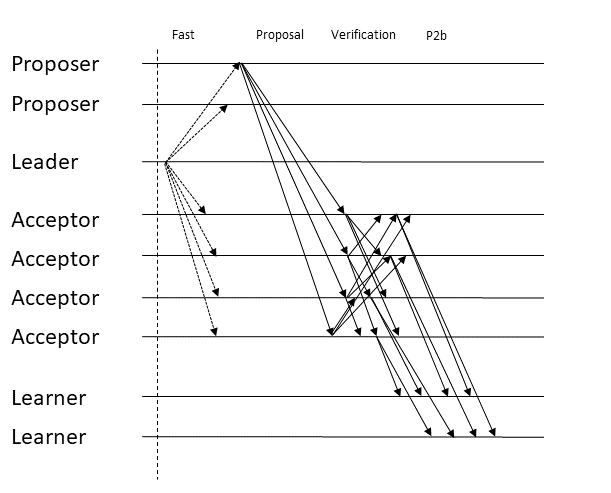
\includegraphics[width=.6\textwidth]{Figures/bgp_fast}
\caption{{BGP's} fast ballot message pattern.} %We moved it close to its first mention, please confirm.
\label{bgp_fast}
\end{figure}
\unskip
\begin{figure}
\centering
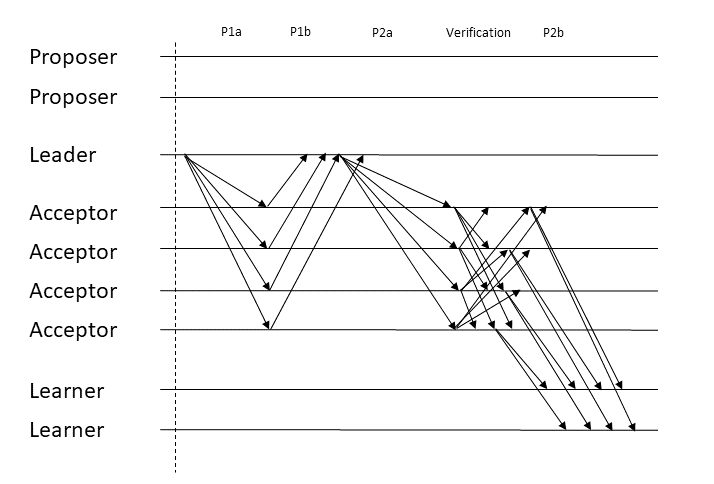
\includegraphics[width=.6\textwidth]{Figures/bgp_classic}
\caption{{BGP's} classic ballot message pattern.}%We moved it close to its first mention, please confirm.
\label{bgp_classic}
\end{figure}
\unskip
\begin{algorithm}[H] 
\setstretch{1.35}\small
\caption{Byzantine Generalized Paxos---Acceptor a (view change)}
\label{BFT-Proc}
\textbf{Local variables:} $suspicions = \bot,\ new\_view = \bot,\ leader = \bot,\ view = 0, bal_a = 0, \ val_a = \bot,\ fast\_bal = \bot,\ checkpoint=\bot$
\begin{algorithmic}[1] 
\State \textbf{upon} \textit{suspect\_leader} \textbf{do} 
\State\hspace{\algorithmicindent} \textbf{if} $suspicions[p] \neq true$ \textbf{then}
\State\hspace{\algorithmicindent}\hspace{\algorithmicindent} $suspicions[p] = true$
\State\hspace{\algorithmicindent}\hspace{\algorithmicindent} $proof = \langle suspicion, view \rangle_{priv_a}$
\State \hspace{\algorithmicindent}\hspace{\algorithmicindent} $\Call{send}{SUSPICION, view,proof}$
\State
\State \textbf{upon} \textit{receive($SUSPICION, view_i, proof$)} from acceptor $i$ \textbf{do} 
\State\hspace{\algorithmicindent} \textbf{if} $view_i \neq view$ \textbf{then}
\State\hspace{\algorithmicindent}\hspace{\algorithmicindent} \textbf{return}
\State\hspace{\algorithmicindent} \textbf{if} $proof_{pub_i} == \langle suspicion, view \rangle$ \textbf{then}
\State\hspace{\algorithmicindent}\hspace{\algorithmicindent} $suspicions[i] = proof$
\State\hspace{\algorithmicindent} \textbf{if} $\#(suspicions) > f$ and $new\_view[view+1][p] == \bot$ \textbf{then}
\State\hspace{\algorithmicindent}\hspace{\algorithmicindent} $change\_proof = \langle view\_change, view +1 \rangle_{priv_a}$
\State\hspace{\algorithmicindent}\hspace{\algorithmicindent} $new\_view[view+1][p] = change\_proof$
\State\hspace{\algorithmicindent}\hspace{\algorithmicindent} $\Call{send}{VIEW\_CHANGE, view+1, suspicions, change\_proof}$
\State
\State\textbf{upon} \textit{receive($VIEW\_CHANGE, new\_view_i, suspicions, change\_proof_i$)} from acceptor $i$ \textbf{do} 
\State\hspace{\algorithmicindent} \textbf{if} $new\_view_i \leq view$ \textbf{then}
\State\hspace{\algorithmicindent}\hspace{\algorithmicindent}\textbf{return}
\State
\State\hspace{\algorithmicindent} $valid\_proofs = 0$
\State\hspace{\algorithmicindent} \textbf{for} $p$ \textbf{in} $acceptors$ \textbf{do} 
\State\hspace{\algorithmicindent}\hspace{\algorithmicindent} $proof = suspicions[p]$
\State\hspace{\algorithmicindent}\hspace{\algorithmicindent} $last\_view = new\_view_i-1$
\State\hspace{\algorithmicindent}\hspace{\algorithmicindent} \textbf{if} $proof_{pub_p} == \langle suspicion, last\_view \rangle$ \textbf{then}
\State\hspace{\algorithmicindent}\hspace{\algorithmicindent}\hspace{\algorithmicindent} $valid\_proofs \mathrel{+{=}} 1$
\State
\State\hspace{\algorithmicindent} \textbf{if} $valid\_proofs \leq f$ \textbf{then}
\State\hspace{\algorithmicindent}\hspace{\algorithmicindent} \textbf{return}
\State
\State\hspace{\algorithmicindent} $new\_view[new\_view_i][i] = change\_proof_i$
\State\hspace{\algorithmicindent} \textbf{if} $new\_view[view_i][a] == \bot$ \textbf{then} 
\State\hspace{\algorithmicindent}\hspace{\algorithmicindent} $change\_proof = \langle view\_change, new\_view_i \rangle_{priv_a}$
\State\hspace{\algorithmicindent}\hspace{\algorithmicindent} $new\_view[view_i][a] = change\_proof$
\State\hspace{\algorithmicindent}\hspace{\algorithmicindent} $\Call{send}{VIEW\_CHANGE, view_i, suspicions, change\_proof}$
\State
\State\hspace{\algorithmicindent} \textbf{if} $\#(new\_view[new\_view_i]) \geq N-f$ \textbf{then}
\State\hspace{\algorithmicindent}\hspace{\algorithmicindent} $view = view_i$
\State\hspace{\algorithmicindent}\hspace{\algorithmicindent} $leader = view\ mod\ N$
\State\hspace{\algorithmicindent}\hspace{\algorithmicindent} $suspicions = \bot$
\State\hspace{\algorithmicindent}\hspace{\algorithmicindent} $\Call{send}{LEADER, view, new\_view[view_i]}$ to leader
\end{algorithmic}
\end{algorithm}

\subsubsection{Fast Ballots} 


Fast ballots leverage the weaker specification of generalized consensus (compared to classic consensus) in terms of command ordering at different replicas, to~allow for the faster execution of commands in some cases. The~basic idea of fast ballots is that proposers contact the acceptors directly, bypassing the leader, and~then the acceptors send their vote for the current sequence to the learners. If~a conflict exists and progress is not being made, the~protocol reverts to using a classic ballot. This~is where generalized consensus allows us to avoid falling back to this slow path, namely in the case where commands that ordered differently at different acceptors commute. \par 
However, this concurrency introduces safety problems even when a quorum is reached for some sequence. If~we keep the original Fast Paxos message pattern~\cite{L06}, it is possible for one sequence $s$ to be learned at one learner $l_1$ while another non-commutative sequence $s'$ is learned before $s$ at another learner $l_2$. Suppose~$s$ obtains a quorum of votes and is learned by $l_1$ but the same votes are delayed indefinitely before reaching $l_2$. In~the next classic ballot, when the leader gathers a quorum of \textit{phase~1b} messages it must arbitrate an order for the commands that it received from the acceptors and it does not know the order in which they were learned. This~is because, of~the $N-f$ messages it received, $f$ may not have participated in the quorum and another $f$ may be Byzantine and lie about their vote, which only leaves one correct acceptor that participated in the quorum and a single vote is not enough to determine if the sequence was learned or not. If~the leader picks the wrong sequence, it~would be proposing a sequence $s'$ that is non-commutative to a learned sequence $s$. Since~the learning of $s$ was delayed before reaching $l_2$, $l_2$ could learn $s'$ and be in a conflicting state with respect to $l_1$, violating consistency. In~order to prevent this, sequences accepted by a quorum of acceptors must be monotonic extensions of previous accepted sequences. Regardless~of the order in which a learner learns a set of monotonically increasing sequences, the~resulting state will be the same. The~additional verification phase is what allows acceptors to prove to the leader that some sequence was accepted by a quorum. By~gathering $N-f$ proofs for some sequence, an~acceptor can prove that at least $f+1$ correct acceptors voted for that sequence. Since~there are only another $2f$ acceptors in the system, no~other non-commutative value may have been voted for by a quorum. \par
% An interesting alternative to requiring $N-f$ proofs from each acceptor, would be for the leader to wait for $2f+1$ matching \textit{phase 1b} messages. Since~at least $f+1$ of those would be correct, only that sequence could've been learned since any other non-commutative sequence would obtain at most $2f$ votes. Zyzzyva~uses a similar approach of waiting for $3f+1$ to commit requests in single round-trip in executions where no faults occur~\cite{Kotla:2008}. However,~this approach is unsuitable for BGP since it is possible for a sequence to be chosen by a quorum without the leader being aware of more than $f+1$ votes in its quorum. Since~$f+1$ votes aren't enough to ensure the leader that the sequence was chosen by a quorum, the~leader wouldn't be able to pick a learned sequence.\par
Next, we~explain each of the protocol's steps for fast ballots in greater detail.

{\bf Step 1: Proposer to acceptors}.
To initiate a fast ballot, the~leader informs both proposers and acceptors that the proposals may be sent directly to the acceptors. Unlike~classic ballots, where the sequence proposed by the leader consists of the commands received from the proposers appended to previously proposed commands, in~a fast ballot, proposals can be sent to the acceptors in the form of either a single command or a sequence to be appended to the command history. These~proposals are sent directly from the proposers to the acceptors.

{\bf Step 2: Acceptors to acceptors}.
Acceptors append the proposals they receive to the proposals they have previously accepted in the current ballot and broadcast the resulting sequence and the current ballot to the other acceptors, along with a signed tuple of these two values. Intuitively,~this broadcast corresponds to a verification phase where acceptors gather proofs that a sequence gathered enough support to be committed. These~proofs will be sent to the leader in the subsequent classic ballot in order for it to pick a sequence that preserves consistency. To~ensure safety, correct learners must learn non-commutative commands in a total order. When~an acceptor gathers $N-f$ proofs for equivalent values, it~proceeds to the next phase. That~is, sequences do not necessarily have to be equal in order to be learned since commutative commands may be reordered. Recall~that a sequence is equivalent to another if it can be transformed into the second one by reordering its elements without changing the order of any pair of non-commutative commands (in the pseudocode, proofs for equivalent sequences are being treated as belonging to the same index of the \emph{proofs} variable, to~simplify the presentation). By~requiring $N-f$ votes for a sequence of commands, we~ensure that, given two sequences where non-commutative commands are differently ordered, only one sequence will receive enough votes even if $f$ Byzantine acceptors vote for both sequences. Outside~the set of (up to) $f$ Byzantine acceptors, the~remaining $2f+1$ correct acceptors will only vote for a single sequence, which means there are only enough correct processes to commit one of them. As in the non-Byzantine protocol, the fact that proposals are sent as extensions to previous sequences makes the protocol robust against the network reordering of non-commutative commands. 

\begin{algorithm}[H] 
\setstretch{1.35}
\caption{Byzantine Generalized Paxos---Acceptor a (agreement)}
\label{BFT-Acc}
\textbf{Local variables:} $leader = \bot,\ view = 0, bal_a = 0,\ val_a = \bot,\ fast\_bal = \bot,\ proven = \bot$
\begin{algorithmic}[1]
\State \textbf{upon} \textit{receive($P1A, ballot, view_l$)} from leader $l$ \textbf{do}
\State \hspace{\algorithmicindent} \textbf{if} $view_l == view$ and $bal_a < ballot$ \textbf{then}
\State \hspace{\algorithmicindent}\hspace{\algorithmicindent} $\Call{send}{P1B, ballot,bal_a,proven, val_a, proofs[bal_a]}$ to leader
\State \hspace{\algorithmicindent}\hspace{\algorithmicindent} $bal_a = ballot$
\State \hspace{\algorithmicindent}\hspace{\algorithmicindent} $val_a = \bot$ 
\State
\State \textbf{upon} \textit{receive($FAST,ballot,view_l$)} from leader \textbf{do}
\State \hspace{\algorithmicindent} \textbf{if} $view_l == view$ \textbf{then}
\State \hspace{\algorithmicindent}\hspace{\algorithmicindent} $fast\_bal[ballot] = true$

\State
\State \textbf{upon} \textit{receive($VERIFY,view_i, ballot_i,val_i,proof$)} from acceptor $i$ \textbf{do}
\State \hspace{\algorithmicindent} \textbf{if} $proof_{pub_i} == \langle ballot_i, val_i \rangle$ and $view == view_i$ \textbf{then}
\State \hspace{\algorithmicindent}\hspace{\algorithmicindent} $proofs[ballot_i][val_i][i] = proof$
\State \hspace{\algorithmicindent}\hspace{\algorithmicindent} \textbf{if} $\#(proofs[ballot_i][val_i]) \geq N-f$ \textbf{then}
\State \hspace{\algorithmicindent}\hspace{\algorithmicindent}\hspace{\algorithmicindent} $proven = val_i$
\State \hspace{\algorithmicindent}\hspace{\algorithmicindent}\hspace{\algorithmicindent} $\Call{send}{P2B, ballot_i, val_i, proofs[ballot_i][value_i]}$ to learners
\State
\State \textbf{upon} \textit{receive$(P2A\_CLASSIC, ballot, view, value$)} from leader \textbf{do}
\State \hspace{\algorithmicindent} \textbf{if} $view_l == view$ \textbf{then}
\State \hspace{\algorithmicindent}\hspace{\algorithmicindent} $\Call{phase\_2b\_classic}{ballot, value}$
\State 
\State \textbf{upon} \textit{receive($P2A\_FAST, value$)} from proposer \textbf{do}
\State \hspace{\algorithmicindent} $\Call{phase\_2b\_fast}{value}$
\State
\Function{phase\_2b\_classic}{$ballot, value$}
\State $univ\_commut = \Call{isUniversallyCommutative}{val_a}$
\State \textbf{if} $ballot \geq bal_a$ and $val_a == \bot$ and \ $!fast\_bal[bal_a]$ and ($univ\_commut$ or $proven == \bot$ or $proven == \Call{subsequence}{value, 0, \#(proven)}$) \textbf{then}
\State \hspace{\algorithmicindent} $bal_a = ballot$
\State \hspace{\algorithmicindent} \textbf{if} $univ\_commut$ \textbf{then}
\State \hspace{\algorithmicindent}\hspace{\algorithmicindent} $\Call{send}{P2B,bal_a, value}$ to learners
\State \hspace{\algorithmicindent} \textbf{else} 
\State \hspace{\algorithmicindent}\hspace{\algorithmicindent} $val_a = value$
\State \hspace{\algorithmicindent}\hspace{\algorithmicindent} $proof = \langle ballot, val_a \rangle_{priv_a}$
\State \hspace{\algorithmicindent}\hspace{\algorithmicindent} $proofs[ballot][val_a][a] = proof$
\State \hspace{\algorithmicindent}\hspace{\algorithmicindent} $\Call{send}{VERIFY, view, ballot, val_a, proof}$ to acceptors
\EndFunction
\State
\Function{phase\_2b\_fast}{$ballot, value$}
\State \textbf{if} $ballot == bal_a$ and $fast\_bal[bal_a]$ \textbf{then}
\State \hspace{\algorithmicindent} \textbf{if} $\Call{isUniversallyCommutative}{value}$ \textbf{then}
\State \hspace{\algorithmicindent}\hspace{\algorithmicindent} $\Call{send}{P2B,bal_a, value}$ to learners
\State \hspace{\algorithmicindent} \textbf{else}
\State \hspace{\algorithmicindent}\hspace{\algorithmicindent} $val_a = val_a \bullet value$
\State \hspace{\algorithmicindent}\hspace{\algorithmicindent} $proof = \langle ballot, val_a \rangle_{priv_a}$
\State \hspace{\algorithmicindent}\hspace{\algorithmicindent} $proofs[ballot][val_a][a] = proof$
\State \hspace{\algorithmicindent}\hspace{\algorithmicindent} $\Call{send}{VERIFY, view, ballot, val_a, proof}$ to acceptors
\EndFunction
\end{algorithmic}
\end{algorithm}


{\bf Step 3: Acceptors to learners}. Similarly to what happens in classic ballots, the~fast ballot equivalent of the \textit{phase 2b} message, which is sent from acceptors to learners, contains the current ballot number, the~command sequence and the $N-f$ proofs gathered in the verification round. One~could think that, since acceptors are already gathering proofs that a value will eventually be committed, learners are not required to gather $N-f$ votes and they can wait for a single \textit{phase 2b} message and validate the $N-f$ proofs contained in it. However,~this is not the case due to the possibility of learners learning sequences without the leader being aware of it. If~we allowed the learners to learn after witnessing $N-f$ proofs for just one acceptor then that would raise the possibility of that acceptor not being present in the quorum of \textit{phase 1b} messages. Therefore,~the~leader wouldn't be aware that some value was proven and learned. The~only way to guarantee that at least one correct acceptor will relay the latest proven sequence to the leader is by forcing the learner to require $N-f$ \textit{phase 2b} messages since only then will one correct acceptor be in the intersection of the two quorums. 

{\bf Arbitrating an order after a conflict}. When, in~a fast ballot, non-commutative commands are concurrently proposed, these commands may be incorporated into the sequences of various acceptors in different orders and, therefore, the~sequences sent by the acceptors in \textit{phase 2b} messages will not be equivalent and will not be learned. In~this case, the~leader subsequently runs a classic ballot and gathers these unlearned sequences in \textit{phase 1b}. Then,~the~leader will arbitrate a single serialization for every previously proposed command, which it will then send to the acceptors. Therefore,~if~non-commutative commands are concurrently proposed in a fast ballot, they will be included in the subsequent classic ballot and the learners will learn them in a total order, thus preserving consistency.

\subsubsection{Classic Ballots} 

Classic ballots work in a way that is very close to the original Paxos protocol~\cite{Lam98}. Therefore,~throughout our description, we~will highlight the points where BGP departs from that original protocol, either due to the Byzantine fault model, or~due to behaviors that are particular to our specification of the consensus problem.\par

In this part of the protocol, the~leader continuously collects proposals by assembling all commands that are received from the proposers since the previous ballot in a sequence (this differs from classic Paxos, where it suffices to keep a single proposed value that the leader attempts to reach agreement~on). When~the next ballot is triggered, the~leader starts the first phase by sending \textit{phase 1a} messages to all acceptors containing just the ballot number. Similarly~to classic Paxos, acceptors reply with a \textit{phase 1b} message to the leader, which reports all sequences of commands they voted for. In~classic Paxos, acceptors also promise not to participate in lower-numbered ballots, in~order to prevent safety violations~\cite{Lam98}. However,~in~BGP this promise is already implicit, given (1) there is only one leader per view and it is the only process allowed to propose in a classic ballot and (2) acceptors replying to that message must be in the same view as that leader.

As previously mentioned, \textit{phase 1b} messages contain $N-f$ proofs for each learned sequence. By~waiting for $N-f$ such messages, the~leader is guaranteed that, for~any learned sequence $s$, at~least one of the messages will be from a correct acceptor that, due~to the quorum intersection property, participated in the verification phase of $s$. Please note~that waiting for $N-f$ \textit{phase 1b} messages is not what makes the leader be sure that a certain sequence was learned in a previous ballot. The~leader can be sure that some sequence was learned because each \textit{phase 1b} message contains cryptographic proofs from $2f+1$ acceptors stating that they would vote for that sequence. Since~there are only $3f+1$ acceptors in the system, no~other non-commutative sequence could have been learned. Even~though each \textit{phase 1b} message relays enough proofs to ensure the leader that some sequence was learned, the~leader still needs to wait for $N-f$ such messages to be sure that he is aware of any sequence that was previously learned. Please note~that, since each command is signed by the proposer (this signature and its check are not explicit in the pseudocode), a~Byzantine acceptor cannot relay made-up commands. However,~it~can omit commands from its \textit{phase 1b} message, which is why it is necessary for the leader to be sure that at least one correct acceptor in its quorum took part in the verification quorum of any learned sequence. \par
After gathering a quorum of $N-f$ \textit{phase 1b} messages, the~leader initiates \textit{phase 2a} where it assembles a proposal and sends it to the acceptors. This~proposal sequence must be carefully constructed in order to ensure all of the intended properties. In~particular, the~proposal cannot contain already learned non-commutative commands in different relative orders than the one in which they were learned, in~order to preserve consistency, and~it must contain unlearned proposals from both the current and the previous ballots, in~order to preserve liveness (this differs from sending a single value with the highest ballot number as in the classic specification). Due~to the importance and required detail of the leader's value picking rule, it~will be described next in its own subsection. \par
The acceptors reply to \textit{phase 2a} messages by broadcasting their verification messages containing the current ballot, the~proposed sequence and proof of their committal to that sequence. After~receiving $N-f$ verification messages, an~acceptor sends its \textit{phase 2b} messages to the learners, containing the ballot, the~proposal from the leader and the $N-f$ proofs gathered in the verification phase. As~is the case in the fast ballot, when a learner receives a \textit{phase 2b} vote, it~validates the $N-f$ proofs contained in it. Waiting~for a quorum of $N-f$ messages for a sequence ensures the learners that at least one of those messages was sent by a correct acceptor that will relay the sequence to the leader in the next classic ballot (the learning of sequences also differs from the original protocol in the quorum size, due~to the fault model, and~in that the learners would wait for a quorum of matching values instead of equivalent sequences, due~to the consensus specification.)\par

\subsubsection{Leader Value Picking Rule} \textit{Phase 2a} is crucial for the correct functioning of the protocol because it requires the leader to pick a value that allows new commands to be learned, ensuring progress, while at the same time preserving a total order of non-commutative commands at different learners, ensuring consistency. The~value picked by the leader is composed of three pieces: (1) the subsequence that has proven to be accepted by a majority of acceptors in the previous fast ballot, (2) the subsequence that has been proposed in the previous fast ballot but for which a quorum hasn't been gathered and (3) new proposals sent to the leader in the current classic ballot. \par
The first part of the sequence will be the largest of the $N-f$ proven sequences sent in the \textit{phase 1b} messages. The~leader can pick such a value deterministically because, for~any two proven sequences, they are either equivalent or one can be extended to the other. The~leader is sure of this because for the quorums of any two proven sequences there is at least one correct acceptor that voted in both and votes from correct acceptors are always extensions of previous votes from the same ballot. If~there are multiple sequences with the maximum size then they are equivalent (by same reasoning applied previously) and any can be picked. \par
The second part of the sequence is simply the concatenation of unproven sequences of commands in an arbitrary order. Since~these commands are guaranteed to not have been learned at any learner, they can be appended to the leader's sequence in any order. Since~$N-f$ \textit{phase 2b} messages are required for a learner to learn a sequence and the intersection between the leader's quorum and the quorum gathered by a learner for any sequence contains at least one correct acceptor, the~leader can be sure that if a sequence of commands is unproven in all of the gathered \textit{phase 1b} messages, then that sequence wasn't learned and can be safely appended to the leader's sequence in any order. \par 
The third part consists simply of commands sent by proposers to the leader with the intent of being learned at the current ballot. These~values can be appended in any order and without any restriction since they're being proposed for the first time.

\begin{algorithm}[H]
\setstretch{1.35}
\caption{Byzantine Generalized Paxos---Learner l}
\label{BFT-Learn}
\textbf{Local variables:} $learned = \bot, messages = \bot$
\begin{algorithmic}[1] 
\State \textbf{upon} \textit{receive($P2B, ballot, value, proofs$)} from acceptor $a$ \textbf{do}
\State \hspace{\algorithmicindent} $valid\_proofs = 0$
\State \hspace{\algorithmicindent} \textbf{for} $i$ \textbf{in} $acceptors$ \textbf{do}
\State \hspace{\algorithmicindent}\hspace{\algorithmicindent} $proof = proofs[i]$
\State \hspace{\algorithmicindent}\hspace{\algorithmicindent} \textbf{if} $proof_{pub_i} == \langle ballot, value \rangle$ \textbf{then}
\State \hspace{\algorithmicindent}\hspace{\algorithmicindent}\hspace{\algorithmicindent} 
$valid\_proofs \mathrel{+{=}} 1$
\State
\State \hspace{\algorithmicindent} \textbf{if} $valid\_proofs \geq N-f$ \textbf{then}
\State \hspace{\algorithmicindent}\hspace{\algorithmicindent} $messages[ballot][value][a] = proofs$
\State
\State \hspace{\algorithmicindent}\hspace{\algorithmicindent} \textbf{if} $\#(messages[ballot][value]) \geq N-f$ \textbf{then}
\State \hspace{\algorithmicindent}\hspace{\algorithmicindent}\hspace{\algorithmicindent} $learned = \Call{merge\_sequences}{learned, value}$

\State
\State \textbf{upon} \textit{receive($P2B, ballot, value$)} from acceptor $a$ \textbf{do}
\State \hspace{\algorithmicindent} \textbf{if} $\Call{isUniversallyCommutative}{value}$ \textbf{then}
\State \hspace{\algorithmicindent}\hspace{\algorithmicindent}
$messages[ballot][value][a] = true$
\State \hspace{\algorithmicindent}\hspace{\algorithmicindent} \textbf{if} $\#(messages[ballot][value]) > f$ \textbf{then} 
\State \hspace{\algorithmicindent}\hspace{\algorithmicindent}\hspace{\algorithmicindent} $learned = learned \bullet value$
\State 
\Function{merge\_sequences}{$old\_seq, new\_seq$}
\State \textbf{for} $c$ \textbf{in} $new\_seq$ \textbf{do} 
\State \hspace{\algorithmicindent} \textbf{if} $!\Call{contains}{old\_seq,c}$ \textbf{then}
\State \hspace{\algorithmicindent}\hspace{\algorithmicindent}\hspace{\algorithmicindent} $old\_seq = old\_seq \bullet c$
\State \textbf{return} $old\_seq$
\EndFunction
\end{algorithmic}
\end{algorithm}

\subsubsection{Byzantine Leader}
The correctness of the protocol is heavily dependent on the guarantee that the sequence accepted by a quorum of acceptors is an extension of previous 
proven sequences. Otherwise,~if~the network rearranges \textit{phase 2b} messages such that they're seen by different learners in different orders, they will result in a state divergence. If,~however, every vote is a prefix of all subsequent votes then, regardless of the order in which the sequences are learned, the~final state will be the same. \par 
This state equivalence between learners is ensured by the correct execution of the protocol since every vote in a fast ballot is equal to the previous vote with a sequence appended at the end (Algorithm~\ref{BFT-Acc} lines \{43--46\}) and every vote in a classic ballot is equal to all the learned votes concatenated with unlearned votes and new proposals (Algorithm~\ref{BFT-Lead} lines \{42--45\}) which means that new votes will be extensions of previous proven sequences. However,~this begs the question of how the protocol fares when Byzantine faults occur. In~particular, the~worst case scenario occurs when both $f$ acceptors and the leader are Byzantine (remember that a process can have multiple roles, such as leader and acceptor). In~this scenario, the~leader can purposely send \textit{phase 2a} messages for a sequence that is not prefixed by the previously accepted values. Coupled~with an asynchronous network, this malicious message can be delivered before the correct votes of the previous ballot, resulting in different learners learning sequences that may not be extensible to equivalent sequences. \par
To prevent this scenario, the~acceptors must ensure that the proposals they receive from the leader are prefixed by the values they have previously voted for. Since~an acceptor votes for its $val_a$ sequence after receiving $N-f$ verification votes for an equivalent sequence and stores it in its $proven$ variable, the~acceptor can verify that it is a prefix of the leader's proposed value (i.e., $proven \sqsubseteq value$). A~practical implementation of this condition is simply to verify that the subsequence of $value$ starting at the index $0$ up to index $length(proven)-1$ is equivalent to the acceptor's $proven$ sequence. 


\subsection{Checkpointing} BGP includes an additional feature that deals with the indefinite accumulation of state at the acceptors and learners. This~is of great practical importance since it can be used to prevent the storage of commands sequences from depleting the system's resources. This~feature is implemented by a special command $C^*$, proposed by the leader, which causes both acceptors and learners to safely discard previously stored commands. However,~the~reason acceptors accumulate state continuously is because each new proven sequence must contain any previous proven sequence. This~ensures that an asynchronous network cannot reorder messages and cause learners to learn in different orders. In~order to safely discard state, we~must implement a mechanism that allows us to deal with reordered messages that do not contain the entire history of learned commands.\par
To this end, when a learner learns a sequence that contains a checkpointing command $C^*$ at the end, it~discards every command in its $learned$ sequence except $C^*$ and sends a message to the acceptors notifying them that it executed the checkpoint for some command $C^*$. Acceptors~stop participating in the protocol after sending \textit{phase 2b} messages with checkpointing commands and wait for $N-f$ notifications from learners. After~gathering a quorum of notifications, the~acceptors discard their state, except for the command $C^*$, and~resume their participation in the protocol. Please note~that since the acceptors also leave the checkpointing command in their sequence of proven commands, every valid subsequent sequence will begin with $C^*$. The~purpose of this command is to allow a learner to detect when an incoming message was reordered. The~learner can check the first position of an incoming sequence against the first position of its $learned$ and, if~a mismatch is detected, it~knows that either a pre and post-checkpoint message has been reordered. \par
When performing this check, two~possible anomalies that can occur: either (1) the first position of the incoming sequence contains a $C^*$ command and the learner's $learned$ sequence does not, in~which case the incoming sequence was sent post-checkpoint and the learner is missing a sequence containing the respective checkpoint command; or (2) the first position of the $learned$ sequence contains a checkpoint command and the incoming sequence does not, in~which case the incoming sequence was assembled pre-checkpoint and the learner has already executed the checkpoint. \par
In the first case, the~learner can simply store the post-checkpoint sequences until it receives the sequence containing the appropriate $C^*$ command at which point it can learn the stored sequences. Please note~that the order in which the post-checkpoint sequences are executed is irrelevant since they're extensions of each other. In~the second case, the~learner receives sequences sent before the checkpoint sequence that it has already executed. In~this scenario, the~learner can simply discard these sequences since it knows that it executed a subsequent sequence (i.e., the~one containing the checkpoint command) and proven sequences are guaranteed to be extensions of previous proven sequences. \par
To simplify the algorithm presentation, this extension to the protocol is not included in the pseudocode description.

%\section{Correctness Proofs} \label{proof}

This section argues for the correctness of the Byzantine Generalized Paxos protocol in terms of the specified consensus properties.\par

\begin{table}[h!]
	\renewcommand{\arraystretch}{1.5}
	\centering
	\begin{tabularx}{\linewidth}{ |c|X|}
		%\hline
		%\multicolumn{2}{|c|}{Notation}\\
		\hline
		Invariant/Symbol & Definition \\
		\hline
		$\thicksim$ & Equivalence relation between sequences \\
		\hline
		$X \overset{e}{\implies} Y$ & $X$ implies that $Y$ is eventually true \\
		\hline
		$X \sqsubseteq Y$ & The sequence $X$ is a prefix of sequence $Y$ \\
		\hline
		$\mathcal{L}$ & Set of learner processes \\
		\hline
		$\mathcal{P}$ & Set of proposals (commands or sequences of commands) \\
		\hline
		$learned_{l_i}$ & Learner $l_i$'s $learned$ sequence of commands \\
		\hline
		$learned(l_i,s)$ & $learned_{l_i}$ contains the sequence $s$ \\
		\hline
		$maj\_accepted(s)$ & $N-f$ acceptors sent phase 2b messages to the learners for sequence $s$ \\
		\hline
		$min\_accepted(s)$ & $f+1$ acceptors sent phase 2b messages to the learners for sequence $s$ \\
		\hline
		$proposed(s)$ & A proposer proposed $s$ \\
		\hline
		
	\end{tabularx} 
	\vspace{\smallskipamount}
	\caption{Proof notation} 
	\label{table:1}
\end{table}

\subsubsection{Consistency}
\begin{theorem}At any time and for any two correct learners $l_i$ and $l_j$, $learned_{l_i}$ and $learned_{l_j}$ can subsequently be extended to equivalent sequences \par
\end{theorem} 
\textbf{Proof:} \par
\parbox{\linewidth}{\strut1. At any given instant, $\forall s,s' \in \mathcal{P}, \forall l_i,l_j \in \mathcal{L}, learned(l_j,s) \land learned(l_i,s') \implies \exists \sigma_1,\sigma_2 \in \mathcal{P}, s \thicksim s' \bullet \sigma_1 \lor s' \thicksim s \bullet \sigma_2$}  \par
\indent\indent\parbox{\linewidth}{\strut\textbf{Proof:} }\par
\indent\indent\indent\parbox{\linewidth-\algorithmicindent*3}{\strut1.1. At any given instant, $\forall s,s' \in \mathcal{P}, \forall l_i,l_j \in \mathcal{L}, learned(l_i,s) \land learned(l_j,s') \implies (maj\_accepted(s) \lor (min\_accepted(s) \land (s \thicksim x \bullet \sigma_1 \lor x \thicksim s \bullet \sigma_2))) \land (maj\_accepted(s') \lor (min\_accepted(s') \land (s' \thicksim x \bullet \sigma_1 \lor x \thicksim s' \bullet \sigma_2))), \exists \sigma_1, \sigma_2 \in \mathcal{P}, \forall x \in \mathcal{P}$} \par
\indent\indent\indent\indent\parbox{\linewidth-\algorithmicindent*4}{\strut\textbf{Proof:} A sequence can only be learned if the learner gathers $N-f$ votes (i.e., $maj\_accepted(s)$) or if it is universally commutative (i.e., $s \thicksim x \bullet \sigma_1 \lor x \thicksim s \bullet \sigma_2,\ \exists \sigma_1, \sigma_2 \in \mathcal{P}, \forall x \in \mathcal{P}$) and the learner gathers $f+1$ votes (i.e., $min\_accepted(s)$). The first case includes both gathering $N-f$ votes directly from each acceptor (Algorithm \ref{BFT-Learn} lines \{1-4\}) and gathering $N-f$ proofs of vote from only one acceptor, as is the case when the sequence contains a special checkpointing command (Algorithm \ref{BFT-Learn} \{6-11\}). The second case requires that the sequence must be commutative with any other (Algorithm \ref{BFT-Learn} \{1-4\}). This is encoded in the logical expression $s \thicksim x \bullet \sigma_1 \lor x \thicksim \bullet \sigma_2$ which is true if either the learned sequence $s$ can be extended with a suffix $\sigma_1$ to any other sequence $x$ or if any sequence $x$ can be extended with some prefix $\sigma_2$ to be equivalent to $s$.}
\indent\indent\indent\parbox{\linewidth-\algorithmicindent*3}{\strut1.2. At any given instant, $\forall s,s' \in \mathcal{P}, maj\_accepted(s) \land maj\_accepted(s') \implies \exists \sigma_1,\sigma_2 \in \mathcal{P}, s \thicksim s' \bullet \sigma_1 \lor s' \thicksim s \bullet \sigma_2$}\par
\indent\indent\indent\indent\parbox{\linewidth}{\strut\textbf{Proof:} Proved by contradiction.}\par
\indent\indent\indent\indent\indent\parbox{\linewidth-\algorithmicindent*5}{\strut1.2.1.~At any given instant, $\exists s,s' \in \mathcal{P}, \forall \sigma_1,\sigma_2 \in \mathcal{P}, maj\_accepted(s) \land maj\_accepted(s') \wedge s \not\thicksim s' \bullet \sigma_1 \land s' \not\thicksim s \bullet \sigma_2$} \par
\indent\indent\indent\indent\indent\indent\parbox{\linewidth}{\strut\textbf{Proof:} Contradiction assumption.}\par
\indent\indent\indent\indent\indent\parbox{\linewidth-\algorithmicindent*5}{\strut1.2.2. Take $s$ and $s'$ which are certain to exist by 1.2.1, $s$ and $s'$ are non-commutative }\par
\indent\indent\indent\indent\indent\indent\parbox{\linewidth-\algorithmicindent*6}{\strut\textbf{Proof:} If $\forall \sigma_1,\sigma_2 \in \mathcal{P}, s \not\thicksim s' \bullet \sigma_1 \land s' \not\thicksim s \bullet \sigma_2$ then $s$ and $s'$ must contain non-commutative commands differently ordered. Otherwise, they would be possible to extend to equivalent sequences.}\par
\indent\indent\indent\indent\indent\parbox{\linewidth}{\strut1.2.3. At any given instant, $\neg (maj\_accepted(s) \land maj\_accepted(s'))$ } \par
\indent\indent\indent\indent\indent\indent\parbox{\linewidth-\algorithmicindent*6}{\strut\textbf{Proof:} Since $s$ and $s'$ are non-commutative, therefore not equivalent, and each correct acceptor only votes once for a new proposal (Algorithm \ref{BFT-Acc}, lines \{28-43\}), any learner will only obtain $N-f$ votes for one of the sequences (Algorithm \ref{BFT-Learn}, lines \{1-4\}).}\par
\indent\indent\indent\indent\indent\parbox{\linewidth}{\strut1.2.4. Q.E.D. }\par
\indent\indent\indent\parbox{\linewidth-\algorithmicindent*3}{\strut1.3. Take $s$ and $s'$, at any given instant, $\forall x \in \mathcal{P}, \exists \sigma_1,\sigma_2 \in \mathcal{P}, (maj\_accepted(s) \lor (min\_accepted(s) \land (s \thicksim x \bullet \sigma_1 \lor x \thicksim s \bullet \sigma_2))) \land (maj\_accepted(s') \lor (min\_accepted(s') \land (s' \thicksim x \bullet \sigma_1 \lor x \thicksim s' \bullet \sigma_2))) \implies s \thicksim x \bullet \sigma$}\par
\indent\indent\indent\indent\parbox{\linewidth}{\strut\textbf{Proof:} By 1.2 and by definition of $(s \thicksim x \bullet \sigma \lor x \thicksim s \bullet \sigma)$.}\par
\indent\indent\indent\parbox{\linewidth-\algorithmicindent*3}{\strut1.4. At any given instant, $\forall s,s' \in \mathcal{P}, \forall l_i,l_j \in \mathcal{L}, learned(l_i,s)\ \land\ learned(l_j,s') \implies \exists \sigma_1,\sigma_2 \in \mathcal{P}, s \thicksim s' \bullet \sigma_1 \lor s' \thicksim s \bullet \sigma_2$ }\par
\indent\indent\indent\indent\parbox{\linewidth}{\strut\textbf{Proof:} By 1.1 and 1.3.}\par
\indent\indent\indent\parbox{\linewidth}{\strut1.5. Q.E.D. }\par
\parbox{\linewidth-\algorithmicindent*3}{\strut2. At any given instant, $\forall l_i,l_j \in \mathcal{L}, learned(l_j,learned_j) \land learned(l_i,learned_i) \implies \exists \sigma_1,\sigma_2 \in \mathcal{P}, learned_i \thicksim learned_j \bullet \sigma_1 \lor learned_j \thicksim learned_i \bullet \sigma_2$}\par
\indent\indent\parbox{\linewidth}{\strut\textbf{Proof:} By 1.}\par
\parbox{\linewidth}{\strut3. Q.E.D.} \par

\subsubsection{Non-Triviality}
\begin{theorem}
If all proposers are correct, $learned_l$ can only contain proposed commands. \label{N-T1} \par
\end{theorem} 
\textbf{Proof:} \par
\parbox{\linewidth}{\strut1. At any given instant, $\forall l_i \in \mathcal{L}, \forall s \in \mathcal{P}, learned(l_i,s) \implies \forall x \in \mathcal{P}, \exists \sigma \in \mathcal{P},  maj\_accepted(s) \lor (min\_accepted(s) \land  (s \thicksim x \bullet \sigma \lor x \thicksim s \bullet \sigma))$ }\par
\indent\indent\parbox{\linewidth}{\strut\textbf{Proof:} By Algorithm \ref{BFT-Acc} lines \{28-43\} and Algorithm \ref{BFT-Learn} lines \{1-4,6-11\}, if a correct learner learned a sequence $s$ at any given instant then either $N-f$ or $f+1$ (if $s$ is universally commutative) acceptors must have executed phase $2b$ for $s$.}\par
\parbox{\linewidth}{\strut2. At any given instant, $\forall s \in \mathcal{P}, maj\_accepted(s) \lor min\_accepted(s) \implies proposed(s)$ }\par
\indent\indent\parbox{\linewidth}{\strut\textbf{Proof:} By Algorithm \ref{BFT-Acc} lines \{15-19, 28-43\}, for either $N-f$ or $f+1$ acceptors to accept a proposal it must have been proposed by a proposer.}\par
\parbox{\linewidth}{\strut3. At any given instant, $\forall s \in \mathcal{P}, learned(l_i,s) \implies proposed(s),\forall l_i \in \mathcal{L}$}\par
\indent\indent\parbox{\linewidth}{\strut\textbf{Proof:} By 1 and 2.}\par
\parbox{\linewidth}{\strut4. Q.E.D.}\par

\subsubsection{Stability}
\begin{theorem}
If $learned_l = s$ then, at all later times, $s \sqsubseteq learned_l$, for any sequence $s$ and correct learner $l$ \par \label{S-T1}
\end{theorem} 
\textbf{Proof:} By Algorithm \ref{BFT-Learn} lines \{1-4,6-11\}, a correct learner can only append new commands to its $learned$ command sequence.

\subsubsection{Liveness}
\begin{theorem}
For any proposal $s$ and correct learner $l$, eventually $learned_l$ contains $s$ \label{L-T1} \par
\end{theorem} 
\parbox{\linewidth}{\textbf{Proof:}} \par
\parbox{\linewidth}{\strut1. $\forall\ l_i \in \mathcal{L},\forall s,x \in \mathcal{P}, \exists \sigma \in \mathcal{P}, maj\_accepted(s) \lor (min\_accepted(s) \land  (s \thicksim x \bullet \sigma \lor x \thicksim s \bullet \sigma))\overset{e}{\implies} learned(l_i,s)$}\par
\indent\indent\parbox{\linewidth}{\strut\textbf{Proof:} By Algorithm \ref{BFT-Acc} lines \{28-43\} and Algorithm \ref{BFT-Learn} lines \{1-4,6-11\}, when either $N-f$ or $f+1$ (if $s$ is universally commutative) acceptors accepts a sequence $s$ (or some equivalent sequence), eventually $s$ will be learned by any correct learner.}\par
\parbox{\linewidth}{\strut2. $\forall s \in \mathcal{P}, proposed(s) \overset{e}{\implies} \forall x \in \mathcal{P}, \exists \sigma \in \mathcal{P}, maj\_accepted(s) \lor (min\_accepted(s) \land  (s \thicksim x \bullet \sigma \lor x \thicksim s \bullet \sigma))$} \par
\indent\indent\parbox{\linewidth}{\strut\textbf{Proof:} A proposed sequence is either conflict-free when its incorporated into every acceptor's current sequence or it creates conflicting sequences at different acceptors. In the first case, it's accepted by a quorum (Algorithm \ref{BFT-Acc} lines \{38-43\}) and, in the second case, it's sent in phase $1b$ messages to the in leader in the next ballot (Algorithm \ref{BFT-Acc} lines \{20-26\}) and incorporated in the next proposal (Algorithm \ref{BFT-Lead} lines \{13-18,20-32\}).} \par
\parbox{\linewidth}{\strut3. $\forall l_i \in \mathcal{L}, \forall s \in \mathcal{P}, proposed(s) \overset{e}{\implies} learned(l_i,s)$} \par
\indent\indent\parbox{\linewidth}{\strut\textbf{Proof:} By 1 and 2.} \par
\parbox{\linewidth}{\strut4. Q.E.D.}
\section{Correctness Proofs} \label{bft_proof}

This section argues for the correctness of the Byzantine Generalized Paxos protocol in terms of the specified consensus properties.\par

\begin{table}[H] 
\small\centering
\caption{{BGP} proof notation.}  %This table has not been referred to within the text of the manuscript. Please confirm and give modification.
\label{table:bft_proof} 
%\renewcommand{\arraystretch}{1.5}
\begin{tabular}{cc}
%\hline
%\multicolumn{2}{|c|}{Notation}\\
\toprule
\textbf{Invariant/Symbol} & \textbf{Definition} \\
\midrule
$\thicksim$ & Equivalence relation between sequences \\
%\hline
$X \overset{e}{\implies} Y$ & $X$ implies that $Y$ is eventually true \\
%\hline
$X \sqsubseteq Y$ & The sequence $X$ is a prefix of sequence $Y$ \\
%\hline
$\mathcal{L}$ & Set of learner processes \\
%\hline
$\mathcal{P}$ & Set of proposals (commands or sequences of commands) \\
%\hline
$\mathcal{B}$ & Set of ballots \\
%\hline
$\bot$ & Empty command \\
%\hline 
$learned_{l_i}$ & Learner $l_i$'s $learned$ sequence of commands \\
%\hline
$learned(l_i,s)$ & $learned_{l_i}$ contains the sequence $s$ \\
%\hline
$maj\_accepted(s,b)$ & $N-f$ acceptors sent phase 2b messages to the learners for sequence $s$ in ballot $b$ \\
%\hline
$min\_accepted(s,b)$ & $f+1$ acceptors sent phase 2b messages to the learners for sequence $s$ in ballot $b$\\
%\hline
$proposed(s)$ & A correct proposer proposed $s$ \\
\bottomrule
\end{tabular} 
%\vspace{\smallskipamount}
\end{table}

\subsection{{Consistency}} %Here changed ``\subsubsection'' to be ``\subsection'', please confirm. Same in the below titles (Sections 6.2--6.4), please confirm all.
\begin{Theorem}
At any time and for any two correct learners $l_i$ and $l_j$, $learned_{l_i}$ and $learned_{l_j}$ can subsequently be extended to equivalent sequences. \par
\end{Theorem} 
\noindent\textbf{{Proof:}} \par %Please use the our required proof format, such as the proof format in \subsection{Stability}. Please confirm and give modification.
\parbox{\linewidth-2mm-\algorithmicindent}{\strut1. At~any given instant, $\forall s,s' \in \mathcal{P}, \forall l_i,l_j \in \mathcal{L}, learned(l_j,s) \land learned(l_i,s') \implies \exists \sigma_1,\sigma_2 \in \mathcal{P} \cup \{\bot\}, s~\bullet \sigma_1 \thicksim s' \bullet \sigma_2$} \par
\indent\indent\parbox{\linewidth}{\strut\textbf{Proof:} }\par
\indent\indent\indent\parbox{\linewidth-7mm-\algorithmicindent*3}{\strut1.1. At~any given instant, $\forall s,s' \in \mathcal{P}, \forall l_i,l_j \in \mathcal{L}, learned(l_i,s) \land learned(l_j,s') \implies (maj\_accepted(s,b) \lor (min\_accepted(s,b) \land s \bullet \sigma_1 \thicksim x \bullet \sigma_2)) \land (maj\_accepted(s',b') \lor (min\_accepted(s',b') \land s' \bullet \sigma_1 \thicksim x \bullet \sigma_2)), \exists \sigma_1, \sigma_2 \in \mathcal{P} \cup \{\bot\}, \forall x \in \mathcal{P},\forall b,b' \in \mathcal{B}$} \par
\indent\indent\indent\indent\parbox{\linewidth-9mm-\algorithmicindent*4}{\strut\textbf{Proof:} A sequence can only be learned in some ballot $b$ if the learner gathers $N-f$ votes (i.e., $maj\_accepted(s,b)$), each containing $N-f$ valid proofs, or~if it is universally commutative (i.e., $s \bullet \sigma_1 \thicksim x \bullet \sigma_2,\ \exists \sigma_1, \sigma_2 \in \mathcal{P} \cup \{\bot\}, \forall x \in \mathcal{P}$) and the learner gathers $f+1$ votes (i.e., $min\_accepted(s,b)$). The~first case requires gathering $N-f$ votes from each acceptor and validating that each proof corresponds to the correct ballot and value (Algorithm \ref{BFT-Learn}, lines \{1--12\}). The~second case requires that the sequence must be commutative with any other and at least $f+1$ matching values are gathered (Algorithm \ref{BFT-Learn}, \{14--18\}). This~is encoded in the logical expression $s \bullet \sigma_1 \thicksim x \bullet \sigma_2$ which is true if the accepted sequence $s$ and any other sequence $x$ can be extended to an equivalent sequence, therefore making it impossible to result in a conflict.}

\indent\indent\indent\parbox{\linewidth-7mm-\algorithmicindent*3}{\strut1.2. At~any given instant, $\forall s,s' \in \mathcal{P},\forall b,b' \in \mathcal{B}, maj\_accepted(s,b) \land maj\_accepted(s',b') \implies \exists \sigma_1,\sigma_2 \in \mathcal{P} \cup \{\bot\}, s~\bullet \sigma_1 \thicksim s' \bullet \sigma_2$}\par
\indent\indent\indent\indent\parbox{\linewidth-9mm-\algorithmicindent*4}{\strut\textbf{Proof:} We divide the following proof in two main cases: (1.2.1.) sequences $s$ and $s'$ are accepted in the same ballot $b$ and (1.2.2.) sequences $s$ and $s'$ are accepted in different ballots $b$ and $b'$.}\par
\indent\indent\indent\indent\indent\parbox{\linewidth-11mm-\algorithmicindent*5}{\strut1.2.1.~At any given instant, $\forall s,s' \in \mathcal{P},\forall b \in \mathcal{B}, maj\_accepted(s,b) \land maj\_accepted(s',b) \implies \exists \sigma_1,\sigma_2 \in \mathcal{P} \cup \{\bot\}, s~\bullet \sigma_1 \thicksim s' \bullet \sigma_2$} \par
\indent\indent\indent\indent\indent\indent\parbox{\linewidth}{\strut\textbf{Proof:} Proved by contradiction.}\par
\indent\indent\indent\indent\indent\indent\indent\parbox{\linewidth-15.5mm-\algorithmicindent*7}{\strut1.2.1.1.~At any given instant, $\forall s,s' \in \mathcal{P}, \forall \sigma_1,\sigma_2 \in \mathcal{P} \cup \{\bot \},\forall b \in \mathcal{B}, maj\_accepted(s,b) \land maj\_accepted(s',b) \wedge s \bullet \sigma_1 \not\thicksim s' \bullet \sigma_2$} \par
\indent\indent\indent\indent\indent\indent\indent\indent\parbox{\linewidth}{\strut\textbf{Proof:} Contradiction assumption.}\par
\indent\indent\indent\indent\indent\indent\indent\parbox{\linewidth-15.5mm-\algorithmicindent*7}{\strut1.2.1.2. Take~a pair proposals $s$ and $s'$ that meet the conditions of 1.2.1 (and are certain to exist by the previous point), then $s$ and $s'$ contain non-commutative commands.}\par
\indent\indent\indent\indent\indent\indent\indent\indent\parbox{\linewidth-18mm-\algorithmicindent*8}{\strut\textbf{Proof:} The statement $\forall s,s' \in \mathcal{P}, \forall \sigma_1,\sigma_2 \in \mathcal{P} \cup \{\bot \}, s~\bullet \sigma_1 \not\thicksim s' \bullet \sigma_2$ is trivially false because it implies that, for~any combination of sequences and suffixes, the~extended sequences would never be equivalent. Since~there must be some $s,s',\sigma_1$ and $\sigma_2$ for which the extensions are equivalent (e.g., $s=s'$ and $\sigma_1=\sigma_2$), then the statement is false.}\par
\indent\indent\indent\indent\indent\indent\indent\parbox{\linewidth}{\strut1.2.1.3. A~contradiction is found, Q.E.D. }\par
\indent\indent\indent\indent\indent\parbox{\linewidth-11mm-\algorithmicindent*5}{\strut1.2.2.~At any given instant, $\forall s,s' \in \mathcal{P},\forall b,b' \in \mathcal{B}, maj\_accepted(s,b) \land maj\_accepted(s',b') \land b \neq b' \implies \exists \sigma_1,\sigma_2 \in \mathcal{P} \cup \{\bot\}, s~\bullet \sigma_1 \thicksim s' \bullet \sigma_2$} 
\indent\indent\indent\indent\indent\indent\parbox{\linewidth-13mm-\algorithmicindent*6}{\strut\textbf{Proof:} To prove that values accepted in different ballots are extensible to equivalent sequences, it~suffices to prove that for any sequences $s$ and $s'$ accepted at ballots $b$ and $b'$, respectively, such that $b < b'$ then $s \sqsubseteq s'$. By~Algorithm \ref{BFT-Acc} lines \{11--16, 35, 46\}, any~correct acceptor only votes for a value in variable $val_a$ when it receives $2f+1$ proofs for a matching value. Therefore,~we~prove that a value $val_a$ that receives $2f+1$ verification messages is always an extension of a previous $val_a$ that received $2f+1$ verification messages. By~Algorithm \ref{BFT-Acc} lines \{32, 43\}, $val_a$ only changes when a leader sends a proposal in a classic ballot or when a proposer sends a sequence in a fast ballot.\strut}
\indent\indent\indent\indent\indent\indent\parbox{\linewidth-13mm-\algorithmicindent*6}{\strut In the first case, $val_a$ is substituted by the leader's proposal which means we must prove that this proposal is an extension of any $val_a$ that previously obtained $2f+1$ verification votes. By~Algorithm \ref{BFT-Lead} lines \{24--39, 41--47\}, the~leader's proposal is prefixed by the largest of the proven sequences (i.e., $val_a$ sequences that received $2f+1$ votes in the verification phase) relayed by a quorum of acceptors in \textit{phase 1b} messages. Please note~that, the~verification in Algorithm \ref{BFT-Acc} line \{27\} prevents a Byzantine leader from sending a sequence that is not an extension of previous proved sequences. Since~the verification phase prevents non-commutative sequences from being accepted by a quorum, every proven sequence in a ballot is extensible to equivalent sequences which means that the largest proven sequence is simply the most up-to-date sequence of the previous ballot. \strut}
\indent\indent\indent\indent\indent\indent\parbox{\linewidth-13mm-\algorithmicindent*6}{\strut To prove that the leader can only propose extensions to previous values by picking the largest proven sequence as its proposal's prefix, we~need to assert that a proven sequence is an extension any previous sequence. However,~since that is the same result that we are trying to prove, we~must use induction to do so:\strut}
\indent\indent\indent\indent\indent\indent\indent\parbox{\linewidth-15.5mm-\algorithmicindent*7}{\strut\textbf{1. Base~Case}: In the first ballot, any~proven sequence will be an extension of the empty command $\bot$ and, therefore, an~extension of the previous sequence.\strut}
\indent\indent\indent\indent\indent\indent\indent\parbox{\linewidth-15.5mm-\algorithmicindent*7}{\strut\textbf{2. Induction~Hypothesis}: Assume that, for~some ballot $b$, any~sequence that gathers $2f+1$ verification votes from acceptors is an extension of previous proven sequences.\strut}
\indent\indent\indent\indent\indent\indent\indent\parbox{\linewidth-15.5mm-\algorithmicindent*7}{\strut\textbf{3. Inductive~Step}: By the quorum intersection property, in~a classic ballot $b+1$, the~\textit{phase 1b} quorum will contain ballot $b$'s proven sequences. Given~the largest proven sequence $s$ in the \textit{phase 1b} quorum (which, by~our hypothesis, is~an extension of any previous proven sequences), by~picking $s$ as the prefix of its \textit{phase 2a} proposal (Algorithm \ref{BFT-Lead}, lines \{41--47\}), the~leader will assemble a proposal that is an extension of any previous proven sequence.\strut}
\indent\indent\indent\indent\indent\indent\parbox{\linewidth-13mm-\algorithmicindent*6}{\strut In the second case, a~proposer's proposal $c$ is appended to an acceptor's $val_a$ variable. By~definition of the append operation, $val_a \sqsubseteq val_a \bullet c$ which means that the acceptor's new value $val_a \bullet c$ is an extension of previous~ones.\par}
\indent\indent\indent\parbox{\linewidth-7mm-\algorithmicindent*3}{\strut1.3. For~any pair of proposals $s$ and $s'$, at~any given instant, $\forall x \in \mathcal{P}, \exists \sigma_1,\sigma_2,\sigma_3,\sigma_4 \in \mathcal{P} \cup \{\bot\}, \forall b,b' \in \mathcal{B}, (maj\_accepted(s,b) \lor (min\_accepted(s,b) \land s \bullet \sigma_1 \thicksim x \bullet \sigma_2)) \land (maj\_accepted(s',b') \lor (min\_accepted(s',b') \land s \bullet \sigma_1 \thicksim x \bullet \sigma_2)) \implies s \bullet \sigma_3 \thicksim s' \bullet \sigma_4$}\par
\indent\indent\indent\indent\parbox{\linewidth}{\strut\textbf{Proof:} By 1.2 and by definition of $s \bullet \sigma_1 \thicksim x \bullet \sigma_2$.}\par
\indent\indent\indent\parbox{\linewidth-7mm-\algorithmicindent*3}{\strut1.4. At~any given instant, $\forall s,s' \in \mathcal{P}, \forall l_i,l_j \in \mathcal{L}, learned(l_i,s)\ \land\ learned(l_j,s') \implies \exists \sigma_1,\sigma_2 \in \mathcal{P} \cup \{\bot\}, s~\bullet \sigma_1 \thicksim s' \bullet \sigma_2$ }\par
\indent\indent\indent\indent\parbox{\linewidth}{\strut\textbf{Proof:} By 1.1 and 1.3.}\par
\indent\indent\indent\parbox{\linewidth}{\strut1.5. Q.E.D. }\par
\parbox{\linewidth-7mm-\algorithmicindent*3}{\strut2. At~any given instant, $\forall l_i,l_j \in \mathcal{L}, learned(l_j,learned_j) \land learned(l_i,learned_i) \implies \exists \sigma_1,\sigma_2 \in \mathcal{P} \cup \{\bot\}, learned_i \bullet \sigma_1 \thicksim learned_j \bullet \sigma_2$}\par
\indent\indent\parbox{\linewidth}{\strut\textbf{Proof:} By 1.}\par
\parbox{\linewidth}{\strut3. Q.E.D.} \par

\subsection{Nontriviality}
\begin{Theorem}
If all proposers are correct, $learned_l$ can only contain proposed commands. \label{N-T1} \par
\end{Theorem} 
\noindent\textbf{Proof:} \par
\parbox{\linewidth-2mm-\algorithmicindent}{\strut1. At~any given instant, $\forall l_i \in \mathcal{L}, \forall s \in \mathcal{P}, learned(l_i,s) \implies \forall x \in \mathcal{P}, \exists \sigma \in \mathcal{P}, \forall b \in \mathcal{B}, \ maj\_accepted(s,b) \lor (min\_accepted(s,b) \land (s \thicksim x \bullet \sigma \lor x \thicksim s \bullet \sigma))$ }\par
\indent\indent\parbox{\linewidth-4mm-\algorithmicindent*2}{\strut\textbf{Proof:} By Algorithm \ref{BFT-Acc} lines \{16, 30, 41\} and Algorithm \ref{BFT-Learn} lines \{1--18\}, if~a correct learner learned a sequence $s$ at any given instant then either $N-f$ or $f+1$ (if $s$ is universally commutative) acceptors must have executed \textit{phase 2b} for $s$.}\par
\parbox{\linewidth-2mm-\algorithmicindent}{\strut2. At~any given instant, $\forall s \in \mathcal{P}, \forall b \in \mathcal{B}, maj\_accepted(s,b) \lor min\_accepted(s,b) \implies proposed(s)$ }\par
\indent\indent\parbox{\linewidth-4.5mm-\algorithmicindent*2}{\strut\textbf{Proof:} By Algorithm \ref{BFT-Acc} lines \{18--23\}, for~either $N-f$ or $f+1$ acceptors to accept a proposal it must have been proposed by a proposer (note that the leader is considered a distinguished proposer).}\par
\parbox{\linewidth}{\strut3. At~any given instant, $\forall s \in \mathcal{P}, \forall l_i \in \mathcal{L}, learned(l_i,s) \implies proposed(s)$}\par
\indent\indent\parbox{\linewidth}{\strut\textbf{Proof:} By 1 and 2.}\par
\parbox{\linewidth}{\strut4. Q.E.D.}\par

\subsection{Stability}
\begin{Theorem}
If $learned_l = s$ then, at~all later times, $s \sqsubseteq learned_l$, for~any sequence $s$ and correct learner $l$\looseness=-1. 
\end{Theorem} 
\begin{proof}
By Algorithm \ref{BFT-Learn} lines \{12, 18, 20--26\}, a~correct learner can only append new commands to its $learned$ command sequence.\end{proof}

\subsection{Liveness}
\begin{Theorem}
For any proposal $s$ from a correct proposer, and~correct learner $l$, eventually $learned_l$ contains $s$.\par
\end{Theorem} 
\noindent\parbox{\linewidth}{\textbf{Proof:}} \par
\parbox{\linewidth-2mm-\algorithmicindent}{\strut1. $\forall\ l_i \in \mathcal{L},\forall s,x \in \mathcal{P}, \exists \sigma \in \mathcal{P}, \forall b \in \mathcal{B}, maj\_accepted(s,b) \lor (min\_accepted(s,b) \land (s \thicksim x \bullet \sigma \lor x \thicksim s \bullet \sigma))\overset{e}{\implies} learned(l_i,s)$}\par
\indent\indent\parbox{\linewidth-4.5mm-\algorithmicindent*2}{\strut\textbf{Proof:} By Algorithm \ref{BFT-Acc} lines \{10--15, 28--29, 41--42\} and Algorithm \ref{BFT-Learn} lines \{1--18\}, when either $N-f$ or $f+1$ (if $s$ is universally commutative) acceptors accept a sequence $s$ (or some equivalent sequence), eventually $s$ will be learned by any correct learner.}\par
\parbox{\linewidth-2mm-\algorithmicindent}{\strut2. $\forall s \in \mathcal{P}, proposed(s) \overset{e}{\implies} \forall x \in \mathcal{P}, \exists \sigma \in \mathcal{P}, \forall b \in \mathcal{B}, maj\_accepted(s,b) \lor (min\_accepted(s,b) \land (s \thicksim x \bullet \sigma \lor x \thicksim s \bullet \sigma))$} \par
\indent\indent\parbox{\linewidth-4.5mm-\algorithmicindent*2}{\strut\textbf{Proof:} A proposed sequence is either conflict-free when its incorporated into every acceptor's current sequence or it creates conflicting sequences at different acceptors. In~the first case, it is accepted by a quorum (Algorithm \ref{BFT-Acc}, lines \{10--15, 28--29, 41--42\}) and, in~the second case, it is sent in \textit{phase 1b} messages to the in leader in the next ballot (Algorithm \ref{BFT-Acc}, lines \{1--4\}) and incorporated in the next proposal (Algorithm \ref{BFT-Lead}, lines \{24--47\}).} \par
\parbox{\linewidth}{\strut3. $\forall l_i \in \mathcal{L}, \forall s \in \mathcal{P}, proposed(s) \overset{e}{\implies} learned(l_i,s)$} \par
\indent\indent\parbox{\linewidth}{\strut\textbf{Proof:} By 1 and 2.} \par
\parbox{\linewidth}{\strut4. Q.E.D.}

%\vspace{-0.3cm}

\section{Conclusion and discussion}
\vspace{-0.2cm}
% and Concluding remarks}
\label{sec:disc}
%
We presented a simplified description of the Generalized Paxos specification and protocol, 
and an implementation of Generalized Paxos that is resilient against Byzantine faults.
We now draw some lessons and outline some extensions to our protocol that present interesting directions for future work and hopefully
a better understanding of its practical applicability.

%\shortnegspace

\noindent \textbf{Handling faults in the fast case.}
A result that was stated in the original Generalized Paxos
paper~\cite{Lamport2005} is that to tolerate $f$ crash faults and
allow for fast ballots whenever there are up to $e$ crash faults, the
total system size $N$ must uphold two conditions:
$N > 2f$ and $N > 2e+f$.
Additionally, the fast and classic quorums must be of size $N-e$ and $N-f$, respectively. This implies that there is a price to pay in terms of number of replicas and quorum size for being able to run fast operations during faulty periods.
An interesting observation is that since Byzantine fault tolerance already requires a total system size of $3f+1$ and a quorum size of $2f+1$, we are able to amortize the cost of both features, i.e., we are able to tolerate the maximum number of faults for fast execution without paying a price in terms of the replication factor and quorum size.

%\shortnegspace

\noindent \textbf{Extending the protocol to universally commutative commands.}
% Generalized Paxos vs Paxos spec.
A downside of the use of commutative commands in the
context of Generalized Paxos is that the commutativity check is done
at runtime, to determine if non-commutative commands have
been proposed concurrently.
This raises the possibility of extending the protocol to handle
commands that are universally commutative, i.e., commute with every
other command. For these commands, it is known before executing them
that they will not generate any conflicts, and therefore it is not
necessary to check them against concurrently executing commands.  This
allows us to optimize the protocol by decreasing the number of phase
$2b$ messages required to learn to a smaller $f+1$ quorum. Since, by
definition, these sequences are guaranteed to never produce conflicts,
the $N-f$ quorum is not required to prevent learners from learning
conflicting sequences. Instead, a quorum of $f+1$ is sufficient to
ensure that a correct acceptor saw the command and will eventually
propagate it to a quorum of $N-f$ acceptors. This optimization is particularly useful in the context of 
geo-replicated systems, since it can be significantly faster
to wait for the $f+1$st message instead of the $N-f$th one.

% Weakly consistent replication - also diff order but ok to have different v

\noindent \textbf{Generalized Paxos and weak consistency.}
%The Byzantine Generalized Paxos protocol tackles two challenges in two different avenues of research, fault tolerance and relaxed consistency models. By specifying the generalized consensus problem,
The key distinguishing feature of the specification of Generalized
Paxos~\cite{Lamport2005} is allowing learners to learn concurrent
proposals in a different order, when the proposals commute. This idea
is closely related to the work on weaker consistency models like eventual or
causal consistency~\cite{Ahamad1995}, or consistency models that mix
strong and weak consistency levels like RedBlue~\cite{Li2012}, which attempt
to decrease the cost of executing operations by reducing coordination
requirements between replicas. 
The link between the two models becomes clearer with the introduction of 
universally commutative commands in the previous paragraph.
In the case of weakly consistent replication,
weakly consistent requests can be executed as if they were universally
commutative, even if in practice that may not be the case. E.g., checking 
the balance of a bank account and making a deposit do not commute since
the output of the former depends on their relative order. However,
some systems prefer to run both as weakly consistent operations, even
though it may cause executions that are not explained by a sequential
execution, since the semantics are still acceptable given
that the final state that is reached is the same and no invariants 
of the application are violated~\cite{Li2012}.



% Extension to diff replica grps


%\textbf{Optimizations} One possible optimization of the Byzantine Generalized Paxos protocol leverages universally commutative commands or sequences of commands, which we define as sequences which commute with any other. Universally commutative sequences allows us to reduce latency by decreasing the number of phase $2b$ messages required to learn to a smaller $f+1$ quorum. Since, by definition, these sequences are guaranteed to never produce conflicts, the $N-f$ quorum isn't required to prevent learners from learning conflicting sequences. Instead, a $f+1$ quorum is sufficient for the learner to be sure that the proposed sequence was proposed by a correct proposer. 


% \section{Conclusion}
% \label{sec:conc}
% In this paper, we presented a simplified description of the Generalized Paxos protocol and specification, 
% which is meant to pave the way for new avenues of research in the area. 
% In addition, we modify the protocol to tolerate Byzantine faults, and we prove the correctness of this protocol. 
% In the future, we would like to implement and evaluate the protocol, in addition to gaining a better understanding of its practical applicability.

\section{Conclusions and Discussion}
% and Concluding remarks}
\label{sec:disc}
%
We presented a simplified description of the Generalized Paxos specification and protocol, 
and an implementation of Generalized Paxos that is resilient against Byzantine faults.
We now draw some lessons and outline some extensions to our protocol that present interesting directions for future work and hopefully
a better understanding of its practical applicability.

\subsection{{Handling Faults in the Fast Case}} %We changed ``\paragraph'' to be ``\subsection'', same in the below text, please confirm all.
A result that was stated in the original Generalized Paxos
paper~\cite{Lamport2005} is that to tolerate $f$ crash faults and
allow for fast ballots whenever there are up to $e$ crash faults, the
total system size $N$ must uphold two conditions:
$N > 2f$ and $N > 2e+f$.
Additionally, the~fast and classic quorums must be of size $N-e$ and $N-f$, respectively. This~implies that there is a price to pay in terms of number of replicas and quorum size for being able to run fast operations during faulty periods.
An interesting observation from our work is that, since Byzantine fault tolerance already requires a total system size of $3f+1$ and a quorum size of $2f+1$, we~are able to amortize the cost of both features, i.e., we~are able to tolerate the maximum number of faults for fast execution without paying a price in terms of the replication factor and quorum size.

\subsection{Extending the Protocol to Universally Commutative Commands}
% Generalized Paxos vs Paxos spec.
A downside of the use of commutative commands in the
context of Generalized Paxos is that the commutativity check is done
at runtime, to~determine if non-commutative commands have
been proposed concurrently.
This raises the possibility of extending the protocol to handle
commands that are universally commutative, i.e., commute with every
other command. For~these commands, it~is known before executing them
that they will not generate any conflicts, and~therefore it is not
necessary to check them against concurrently executing commands. This
allows us to optimize the protocol by decreasing the number of phase
$2b$ messages required to learn to a smaller $f+1$ quorum. Since,~by
definition, these sequences are guaranteed to never produce conflicts,
the $N-f$ quorum is not required to prevent learners from learning
conflicting sequences. Instead,~a~quorum of $f+1$ is sufficient to
ensure that a correct acceptor saw the command and will eventually
propagate it to a quorum of $N-f$ acceptors. 
This optimization is particularly useful in the context of 
geo-replicated systems, since it can be significantly faster
to wait for the $f+1$st message instead of the $N-f$th one.\par
The usefulness of this optimization is severely reduced if these sequences are processed like any other, by~being appended to previous sequences at the leader and acceptors. New~proposals are appended to previous proven sequences to maintain the invariant that subsequent proven sequences are extensions of previous ones. Since~the previous proven sequences to which a proposal will be appended to are probably not universally commutative, the~resulting sequence will not be as well. We~can increase this optimization's applicability by sending these sequences immediately to the learners, without appending them to previously accepted ones. This~special handling has the added benefit of bypassing the verification phase, resulting in reduced latency for the requests and less traffic generated per sequence. This~extension can also be easily implemented by adding a single check in Algorithm \ref{BFT-Lead} lines \{19--20\}, Algorithm \ref{BFT-Acc} lines \{29--30, 40--41\} and Algorithm \ref{BFT-Learn} lines \{14--18\}.
% Weakly consistent replication---also diff order but ok to have different v

\subsection{Generalized Paxos and Weak Consistency}
%The Byzantine Generalized Paxos protocol tackles two challenges in two different avenues of research, fault tolerance and relaxed consistency models. By~specifying the generalized consensus problem,
The key distinguishing feature of the specification of Generalized
Paxos~\cite{Lamport2005} is allowing learners to learn concurrent
proposals in a different order, when the proposals commute. This~idea
is closely related to the work on weaker consistency models like eventual or
causal consistency~\cite{Ahamad1995}, or~consistency models that mix
strong and weak consistency levels like RedBlue~\cite{Li2012}, which attempt
to decrease the cost of executing operations by reducing coordination
requirements between replicas. 
The link between the two models becomes clearer with the introduction of 
universally commutative commands in the previous paragraph.
In the case of weakly consistent replication,
weakly consistent requests can be executed as if they were universally
commutative, even if in practice that may not be the case. E.g., checking 
the balance of a bank account and making a deposit do not commute since
the output of the former depends on their relative order. However,
some systems prefer to run both as weakly consistent operations, even
though it may cause executions that are not explained by a sequential
execution, since the semantics are still acceptable given
that the final state that is reached is the same and no invariants 
of the application are violated~\cite{Li2012}.



%%%%%%%%%%%%%%%%%%%%%%%%%%%%%%%%%%%%%%%%%%
%\acknowledgments{\hl{xxx.}}
%%%%%%%%%%%%%%%%%%%%%%%%%%%%%%%%%%%%%%%%%%
%\authorcontributions{\hl{xxx.}}
%For manuscripts with more than one author, please state individual contributions of each author to research and writing of the manuscript.
%%%%%%%%%%%%%%%%%%%%%%%%%%%%%%%%%%%%%%%%%%
\funding{The research of R.\ Rodrigues is funded by the European Research Council (ERC-2012-StG-307732) and by FCT (UID/CEC/50021/2013).}
%Please disclose any funding information, or add "This research received no external funding."
%%%%%%%%%%%%%%%%%%%%%%%%%%%%%%%%%%%%%%%%%%
%\conflictsofinterest{{The authors declare no conflict of interest.}}
%Please disclose conflicts of interest, or add 'The authors declare no conflicts of interest'. 
% Extension to diff replica grps


%\textbf{Optimizations} One possible optimization of the Byzantine Generalized Paxos protocol leverages universally commutative commands or sequences of commands, which we define as sequences which commute with any other. Universally~commutative sequences allows us to reduce latency by decreasing the number of phase $2b$ messages required to learn to a smaller $f+1$ quorum. Since,~by~definition, these sequences are guaranteed to never produce conflicts, the~$N-f$ quorum isn't required to prevent learners from learning conflicting sequences. Instead,~a~$f+1$ quorum is sufficient for the learner to be sure that the proposed sequence was proposed by a correct proposer. 


% \section{Conclusion}
% \label{sec:conc}
% In this paper, we~presented a simplified description of the Generalized Paxos protocol and specification, 
% which is meant to pave the way for new avenues of research in the area. 
% In addition, we~modify the protocol to tolerate Byzantine faults, and~we prove the correctness of this protocol. 
% In the future, we~would like to implement and evaluate the protocol, in~addition to gaining a better understanding of its practical applicability.


\reftitle{References}
\begin{thebibliography}{999}

\bibitem[Pires \em{et~al.}(2017)Pires, Ravi, and~Rodrigues]{Pires2017}
Pires, M.; Ravi, S.; Rodrigues, R.
\newblock Generalized Paxos Made Byzantine (and Less Complex).
\newblock In \emph{Stabilization, Safety, and~Security of Distributed Systems};
Spirakis, P., Tsigas, P., Eds.; Springer International Publishing: Cham, Switzerland, 
2017; pp. 203--218.

\bibitem[Lamport(1998)]{Lam98}
Lamport, L.
\newblock The {Part-Time} Parliament.
\newblock {\em ACM Trans. Comput. Syst.} {\bf 1998}, {\em
16}, 133--169.

\bibitem[Lamport(1989)]{paxos:tr}
Lamport, L.
\newblock \emph{The Part-Time Parliament};
\newblock Technical Report; DEC SRC: {Maynard, MA, USA}, 1989.
%Newly added information, please confirm.

\bibitem[De~Prisco \em{et~al.}(1997)De~Prisco, Lampson, and~Lynch]{DPLL97}
De~Prisco, R.; Lampson, B.; Lynch, N.A.
\newblock Revisiting the {Paxos} Algorithm.
\newblock In \emph{Distributed Algorithms, Proceedings of the 11th Workshop on Distributed Algorithms, Saarbrücken, Germany, 24--26 September 1997}; Springer: {\mbox{Berlin/Heidelberg, Germany}}, %Newly added information, please confirm.
1997; {LNCS 1320}. %Please confirm what it is and please confirm it is correct.

\bibitem[Lee and Thekkath(1996)]{petal}
Lee, E.K.; Thekkath, C.A.
\newblock Petal: Distributed Virtual Disks.
\newblock In Proceedings of the 7th International Conference on Architectural Support for Programming
Languages and Operating Systems, Cambridge, MA, USA, 1--4 October 1996.

\bibitem[Burrows(2006)]{chubby}
Burrows, M.
\newblock The Chubby Lock Service for Loosely-coupled Distributed Systems.
\newblock In Proceedings of the 7th Symposium on Operating Systems Design and Implementation, Seattle, WA, USA, 6--8 November 2006.

\bibitem[Junqueira \em{et~al.}(2011)Junqueira, Reed, and~Serafini]{zookeeper}
Junqueira, F.; Reed, B.; Serafini, M.
\newblock Zab: High-performance Broadcast for Primary-backup Systems.
\newblock In~Proceedings of the 41st International Conference on Dependable Systems and Networks, Hong Kong, China, 27--30 June 2011.

\bibitem[Lamport(2001)]{L01}
Lamport, L.
\newblock Paxos Made Simple.
\newblock {\em SIGACT News} {\bf 2001}, {\em 32}, 18--25.

\bibitem[van Renesse(2011)]{Renesse2011}
van Renesse, R.
\newblock {Paxos Made Moderately Complex}.
\newblock {\em ACM Comput. Surv.} {\bf 2011}, {\em 47}, 1--36.

\bibitem[Castro and Liskov(1999)]{CL99}
Castro, M.; Liskov, B.
\newblock Practical Byzantine Fault Tolerance.
\newblock In Proceedings of the 3rd Symposium on Operating Systems Design and Implementation
(OSDI), New Orleans, LA, USA, 22--25 February 1999.

\bibitem[Lamport(2011)]{Lamport2011}
Lamport, L. Byzantizing Paxos by Refinement.
\newblock In {\em Distributed Computing, Proceedings of the 25th International Symposium (DISC
2011), Rome, Italy, 20--22 September 2011}; Peleg, D., Ed.;
Springer: Berlin/Heidelberg, Germany, 2011; pp. 211--224.

\bibitem[Nakamoto(2008)]{bitcoin}
Nakamoto, S.
\newblock {Bitcoin: A Peer-to-Peer Electronic Cash System. 2008}. %Please add more information to confirm its type, and please use correct format.

\bibitem[Lamport(2006)]{L06}
Lamport, L.
\newblock Fast paxos.
\newblock {\em Distrib. Comput.} {\bf 2006}, {\em 19},~79--103.

\bibitem[Lamport(2005)]{Lamport2005}
Lamport, L.
\newblock \emph{Generalized Consensus and Paxos};
\newblock Microsoft ResearchTechnical Report MSR-TR-2005-33; {2005}. %Please add publisher's name and location.

\bibitem[Ladin \em{et~al.}(1990)Ladin, Liskov, and~Shrira]{LLS90}
Ladin, R.; Liskov, B.; Shrira, L.
\newblock Lazy replication: Exploiting the semantics of Distributed Services.
\newblock In~Proceedings of the 9th Symposium on Principles Distributed Computing, Quebec City, QC, Canada, 22--24 August 1990.

\bibitem[{DeCandia et al.}()]{dynamo}
\textls[-20]{{DeCandia}, G.; Hastorun, D.; Jampani,~M.; Kakulapati,~M.; Lakshman,~A.; Pilchin,~A.; Sivasubramanian,~S.; Vosshall,~P.; Vogels,~W. Dynamo: Amazon's Highly Available Key-value Store. In Proceedings of the 21st ACM SIGOPS Symposium on Operating Systems Principles (SOSP '07), Stevenson, WA, USA, 14--17 October 2007.}

\bibitem[Fischer \em{et~al.}(1985)Fischer, Lynch, and~Paterson]{FLP85}
Fischer, M.J.; Lynch, N.A.; Paterson, M.S.
\newblock Impossibility of Distributed Consensus with one Faulty Process. \emph{J.~ACM}  {\bf
1985},
\newblock {\em 32},~374--382.

\bibitem[Mao \em{et~al.}(2008)Mao, Junqueira, and~Marzullo]{Mao2008}
Mao, Y.; Junqueira, F.P.; Marzullo, K.
\newblock {Mencius: Building Efficient Replicated State Machines for WANs}.
\newblock In~Proceedings of the Symposium on Operating System Design and
Implementation, San Diego, CA, USA, 8--10 December 2008; pp. 369--384.

\bibitem[Moraru \em{et~al.}(2013)Moraru, Andersen, and~Kaminsky]{Moraru2013}
Moraru, I.; Andersen, D.G.; Kaminsky, M.
\newblock {There is more consensus in Egalitarian parliaments}.
\newblock In Proceedings of the Twenty-Fourth ACM Symposium on Operating Systems Principles (Sosp '13), Farminton, PA, USA, 3--6 November 2013;  pp. 358--372.

\bibitem[Lamport \em{et~al.}(1982)Lamport, Shostak, and~Pease]{LSP82}
Lamport, L.; Shostak, R.; Pease, M.
\newblock The {Byzantine} Generals Problem. \emph{ACM Trans. Progr. Lang.~Syst.} {\bf 1982},
\newblock {\em 4}, 382--401.

\bibitem[Dolev \em{et~al.}(1987)Dolev, Dwork, and~Stockmeyer]{Dolev1983}
Dolev, D.; Dwork, C.; Stockmeyer, L.
\newblock On the Minimal Synchronism Needed for Distributed Consensus.
\newblock {\em J.~ACM} {\bf 1987}, {\em 34},~77--97.

\bibitem[Vukolic(2012)]{quorum}
Vukolic, M.
\newblock {\em Quorum Systems: With Applications to Storage and Consensus};
Synthesis Lectures on Distributed Computing Theory, Morgan {\&} Claypool;
{2012}.%Please add publisher's name and location.

\bibitem[Cachin \em{et~al.}(2011)Cachin, Guerraoui, and~Rodrigues]{cgr:book}
Cachin, C.; Guerraoui, R.; Rodrigues, L.E.T.
\newblock {\em Introduction to Reliable and Secure Distributed Programming}, 2nd~ed.; Springer: {\mbox{Berlin/Heidelberg, Germany}}, 2011.
%Newly added information, please confirm.

\bibitem[Lamport(1998)]{Lamport:1998}
{Lamport, L.} %This reference is the same as Ref 2 (\bibitem[Lamport(1998)]{Lam98}), please confirm and give modification.
\newblock The Part-time Parliament.
\newblock {\em ACM Trans. Comput. Syst.} {\bf 1998}, {\em 16},~133--169.

\bibitem[Ahamad \em{et~al.}(1995)Ahamad, Neiger, Burns, Kohli, and
Hutto]{Ahamad1995}
Ahamad, M.; Neiger, G.; Burns, J.E.; Kohli, P.; Hutto, P.W.
\newblock {Causal memory: Definitions, implementation, and~programming}. {In \emph{Distributed Computing}; Springer: \mbox{Berlin/Heidelberg, Germany}}, 
\newblock 1995; Volume~9, pp.~37--49.
%Newly added information, please confirm.

\bibitem[Li \em{et~al.}(2012)Li, Porto, Clement, Gehrke, Pregui{\c{c}}a, and
Rodrigues]{Li2012}
Li, C.; Porto, D.; Clement, A.; Gehrke, J.; Pregui{\c{c}}a, N.; Rodrigues, R.
\newblock {Making Geo-Replicated Systems Fast as Possible, Consistent when
Necessary}.
\newblock In Proceedings of the 10th USENIX Symposium on Operating Systems Design and Implementation (OSDI ’12), Hollywood, CA, USA, 8--10 October 2012.

\end{thebibliography}


\end{document}


